\part*{Auxiliary material}
\addcontentsline{toc}{part}{Auxiliary material}
%-------------------------------------------------------------------------------

%%%%%%%%%%%%%%%%%%%%%%%%
\begin{table}[htbp]
\small
\begin{center}
\begin{tabular}{l*{3}{c}}
\hline\hline
 & 4j, 2b & 4j, 3b & 4j, 4b \\
\hline
$\Hc$ & $ 1990 \pm 190 $ &   $ 1260 \pm 190 $ &   $ 24.8 \pm 9.5 $ \\
$\Hu$ & $ 1950 \pm 190 $ &   $ 1110 \pm 170 $ &   $ 19 \pm 16 $ \\ 
\hline
$\ttbar$+light-jets & $ 87000 \pm 11000 $ &   $ 4300 \pm 1200 $ &   $ 10.2 \pm 9.6 $ \\ 
$\ttcin$ & $ 8300 \pm 4300 $ &   $ 1050 \pm 640 $ &   $ 3.2 \pm 3.3 $ \\ 
$\ttbin$ & $ 3620 \pm 440 $ &   $ 2900 \pm 580 $ &   $ 95 \pm 33 $ \\ 
$t\bar{t}V$ & $ 176 \pm 31 $ &   $ 34.8 \pm 6.9 $ &   $ 2.84 \pm 0.74 $ \\ 
$t\bar{t}H$ & $ 61.7 \pm 9.2 $ &   $ 48.7 \pm 8.3 $ &   $ 5.1 \pm 1.0 $ \\
$W$+jets & $ 5400 \pm 2400 $ &   $ 280 \pm 130 $ &   $ 3.3 \pm 1.8 $ \\ 
$Z$+jets & $ 2120 \pm 960 $ &   $ 115 \pm 55 $ &   $ 2.4 \pm 1.4 $ \\ 
Single top & $ 7100 \pm 1300 $ &   $ 400 \pm 120 $ &   $ 7.8 \pm 6.0 $ \\ 
Diboson & $ 267 \pm 97 $ &   $ 17.2 \pm 6.5 $ &   $ 0.58 \pm 0.27 $ \\ 
Multijet & $ 7800 \pm 3400 $ &   $ 930 \pm 360 $ &   $ 31 \pm 17 $ \\
\hline
Total background & $ 120000 \pm 15000 $ &   $ 10000 \pm 2000 $ &   $ 162 \pm 44 $ \\ 
\hline
Data & 120572  & 11275  & 176  \\
\hline\hline    
\end{tabular}
%%\\
\vspace{0.2cm}

\begin{tabular}{l*{3}{c}}
\hline\hline
 & 5j, 2b & 5j, 3b & 5j, $\geq$4b \\
\hline
$\Hc$ & $ 1260 \pm 240 $ &   $ 1010 \pm 190 $ &   $ 26.2 \pm 8.8 $ \\ 
$\Hu$ & $ 1160 \pm 240 $ &   $ 930 \pm 160 $ &   $ 23 \pm 12 $ \\ 
\hline
$\ttbar$+light-jets & $ 41300 \pm 9100 $ &   $ 3200 \pm 900 $ &   $ 13 \pm 11 $ \\ 
$\ttcin$ & $ 5900 \pm 3100 $ &   $ 1320 \pm 760 $ &   $ 21 \pm 17 $ \\ 
$\ttbin$ & $ 3040 \pm 250 $ &   $ 4300 \pm 760 $ &   $ 310 \pm 83 $ \\ 
$t\bar{t}V$  &   $ 175 \pm 29 $ &   $ 67 \pm 12 $ &   $ 9.1 \pm 2.0 $ \\ 
$t\bar{t}H$  &   $ 81.3 \pm 9.5 $ &   $ 103 \pm 15 $ &   $ 18.4 \pm 3.5 $ \\ 
$W$+jets  &   $ 2400 \pm 1100 $ &   $ 186 \pm 89 $ &   $ 7.3 \pm 3.9 $ \\ 
$Z$+jets  &   $ 780 \pm 350 $ &   $ 83 \pm 39 $ &   $ 6.1 \pm 3.8 $ \\ 
Single top  &   $ 2990 \pm 780 $ &   $ 350 \pm 110 $ &   $ 16.6 \pm 7.6 $ \\ 
Diboson  &   $ 125 \pm 56 $ &   $ 13.7 \pm 6.3 $ &   $ 0.89 \pm 0.47 $ \\ 
Multijet  &   $ 3700 \pm 1500 $ &   $ 500 \pm 230 $ &   $ 3.8 \pm 4.9 $ \\ 
\hline
Total background &  $ 60000 \pm 11000 $ &   $ 10100 \pm 1900 $ &   $ 405 \pm 98 $ \\
\hline
Data & 58557  & 11707  & 466  \\ 
\hline\hline    
\end{tabular}
%%\\
\vspace{0.2cm}

\begin{tabular}{l*{3}{c}}
\hline\hline
 & $\geq$ 6j, 2b & $\geq$6j, 3b & $\geq$6j, $\geq$4b \\
\hline
$\Hc$ & $ 760 \pm 250 $ &   $ 690 \pm 210 $ &   $ 60 \pm 60 $ \\ 
$\Hu$ & $ 680 \pm 240 $ &   $ 570 \pm 180 $ &   $ 36 \pm 40 $ \\ 
\hline
$\ttbar$+light-jets  &   $ 22900 \pm 8100 $ &   $ 2400 \pm 910 $ &   $ 14 \pm 18 $ \\ 
$\ttcin$  &   $ 5300 \pm 3000 $ &   $ 1800 \pm 1100 $ &   $ 29 \pm 23 $ \\ 
$\ttbin$  &   $ 3270 \pm 510 $ &   $ 7300 \pm 1300 $ &   $ 1100 \pm 240 $ \\ 
$t\bar{t}V$  &   $ 229 \pm 41 $ &   $ 154 \pm 30 $ &   $ 30.8 \pm 6.9 $ \\ 
$t\bar{t}H$  &   $ 140 \pm 18 $ &   $ 262 \pm 39 $ &   $ 71 \pm 14 $ \\ 
$W$+jets  &   $ 1360 \pm 630 $ &   $ 200 \pm 100 $ &   $ 15.4 \pm 8.2 $ \\ 
$Z$+jets  &   $ 410 \pm 200 $ &   $ 63 \pm 32 $ &   $ 5.1 \pm 4.0 $ \\ 
Single top  &   $ 1510 \pm 560 $ &   $ 360 \pm 160 $ &   $ 34 \pm 20 $ \\ 
Diboson  &   $ 93 \pm 47 $ &   $ 18.5 \pm 9.6 $ &   $ 2.1 \pm 1.2 $ \\ 
Multijet  &   $ 1920 \pm 820 $ &   $ 780 \pm 360 $ &   $ 43 \pm 29 $ \\ 
\hline
Total background &  $ 37100 \pm 9600 $ &   $ 13400 \pm 2600 $ &   $ 1360 \pm 290 $ \\ 
\hline
Data & 35886  & 14877  & 1335  \\ 
\hline\hline    
\end{tabular}
%%\\
%\vspace{0.2cm}

%
\end{center}
%\vspace{-0.5cm}
\caption{
$\Hbb$ search: Predicted and observed yields in each of the analysis regions considered.
The prediction is shown before the fit to data. Also shown are the signal expectations for 
$\Hc$ and $\Hu$ assuming $\BR(t\to Hc)=1\%$ and $\BR(t\to Hu)=1\%$ respectively.
The quoted uncertainties are the sum in quadrature of statistical and systematic uncertainties of the yields, 
excluding the normalisation uncertainty of the $\ttbin$ background, which is determined via a likelihood fit to data.
}
\label{tab:Hbb_Prefit_Yields_Unblind}
\end{table} 
%%%%%%%%%%%%%%%%%%%%%%%%

%%%%%%%%%%%%%%%%%%%%%%%%
\begin{table}[htbp]
\small
\begin{center}
\begin{tabular}{l*{3}{c}}
\hline\hline
 & 4j, 2b & 4j, 3b & 4j, 4b \\
\hline
$\Hc$  &   $ -30 \pm 470 $ &   $ -20 \pm 300 $ &   $ -0.4 \pm 5.9 $ \\ 
\hline
$\ttbar$+light-jets  &    $ 82900 \pm 4200 $ &   $ 4900 \pm 500 $ &   $ 16 \pm 12 $ \\ 
$\ttcin$  &   $ 11400 \pm 4800 $ &   $ 1360 \pm 550 $ &   $ 5.9 \pm 4.2 $ \\ 
$\ttbin$  &   $ 4270 \pm 590 $ &   $ 3400 \pm 350 $ &   $ 110 \pm 17 $ \\ 
$t\bar{t}V$  &    $ 174 \pm 28 $ &   $ 35.0 \pm 5.9 $ &   $ 2.69 \pm 0.55 $ \\ 
$t\bar{t}H$  &   $ 62.6 \pm 7.8 $ &   $ 47.3 \pm 6.3 $ &   $ 4.68 \pm 0.69 $ \\ 
$W$+jets  &   $ 4800 \pm 1800 $ &   $ 260 \pm 100 $ &   $ 2.9 \pm 1.3 $ \\ 
$Z$+jets  &    $ 1870 \pm 730 $ &   $ 102 \pm 41 $ &   $ 1.9 \pm 1.0 $ \\ 
Single-top  &  $ 6360 \pm 980 $ &   $ 393 \pm 96 $ &   $ 7.6 \pm 5.2 $ \\ 
Diboson  &   $ 242 \pm 84 $ &   $ 16.3 \pm 5.7 $ &   $ 0.50 \pm 0.22 $ \\ 
Multijet  &   $ 9000 \pm 3500 $ &   $ 820 \pm 240 $ &   $ 29 \pm 16 $ \\ 
\hline
Total & $ 121100 \pm 2200 $ &   $ 11290 \pm 280 $ &   $ 181 \pm 23 $ \\ 
\hline
Data & 120572  & 11275  & 176  \\ 
\hline\hline      
\end{tabular}
%%\\
\vspace{0.2cm}

\begin{tabular}{l*{3}{c}}
\hline\hline
 & 5j, 2b & 5j, 3b & 5j, $\geq$4b \\
\hline
$\Hc$  &   $ -20 \pm 300 $ &   $ -10 \pm 240 $ &   $ -0.4 \pm 6.2 $ \\ 
\hline
$\ttbar$+light-jets  &   $ 38000 \pm 3100 $ &   $ 3480 \pm 460 $ &   $ 15.8 \pm 9.5 $ \\ 
$\ttcin$  &   $ 8300 \pm 3400 $ &   $ 2000 \pm 760 $ &   $ 39 \pm 18 $ \\ 
$\ttbin$  &   $ 3410 \pm 470 $ &   $ 4900 \pm 460 $ &   $ 356 \pm 29 $ \\ 
$t\bar{t}V$  &   $ 168 \pm 26 $ &   $ 65 \pm 10 $ &   $ 8.2 \pm 1.4 $ \\ 
$t\bar{t}H$  &   $ 81.1 \pm 8.9 $ &   $ 99 \pm 12 $ &   $ 16.6 \pm 2.3 $ \\ 
$W$+jets  &   $ 2080 \pm 820 $ &   $ 169 \pm 68 $ &   $ 6.0 \pm 2.8 $ \\ 
$Z$+jets  &   $ 700 \pm 270 $ &   $ 74 \pm 30 $ &   $ 5.6 \pm 3.2 $ \\ 
Single-top  &   $ 2560 \pm 590 $ &   $ 322 \pm 90 $ &   $ 13.3 \pm 5.8 $ \\ 
Diboson  &   $ 111 \pm 48 $ &   $ 12.5 \pm 5.4 $ &   $ 0.76 \pm 0.39 $ \\ 
Multijet  &   $ 3380 \pm 950 $ &   $ 560 \pm 230 $ &   $ 3.6 \pm 4.8 $ \\ 
\hline
Total & $ 58800 \pm 1400 $ &   $ 11690 \pm 360 $ &   $ 465 \pm 29 $ \\ 
\hline
Data & 58557  & 11707  & 466  \\ 
\hline\hline      
\end{tabular}
%%\\
\vspace{0.2cm}

\begin{tabular}{l*{3}{c}}
\hline\hline
 & $\geq$6j, 2b & $\geq$6j, 3b & $\geq$6j, $\geq$4b \\
\hline
$\Hc$  &   $ -10 \pm 180 $ &   $ -10 \pm 160 $ &   $ -1 \pm 14 $ \\ 
\hline
$\ttbar$+light-jets  &   $ 20100 \pm 2500 $ &   $ 2560 \pm 490 $ &   $ 21 \pm 23 $ \\ 
$\ttcin$  &   $ 7800 \pm 3300 $ &   $ 3000 \pm 1100 $ &   $ 59 \pm 25 $ \\ 
$\ttbin$  &   $ 3390 \pm 480 $ &   $ 7510 \pm 760 $ &   $ 1106 \pm 83 $ \\ 
$t\bar{t}V$  &   $ 213 \pm 34 $ &   $ 145 \pm 24 $ &   $ 27.0 \pm 4.8 $ \\ 
$t\bar{t}H$  &   $ 134 \pm 15 $ &   $ 240 \pm 30 $ &   $ 61.6 \pm 8.8 $ \\ 
$W$+jets  &   $ 1200 \pm 470 $ &   $ 183 \pm 75 $ &   $ 12.5 \pm 5.7 $ \\ 
$Z$+jets  &   $ 350 \pm 150 $ &   $ 56 \pm 24 $ &   $ 3.5 \pm 2.2 $ \\ 
Single-top  &   $ 1220 \pm 400 $ &   $ 310 \pm 120 $ &   $ 27 \pm 14 $ \\ 
Diboson  &   $ 82 \pm 40 $ &   $ 16.7 \pm 8.2 $ &   $ 1.70 \pm 0.90 $ \\ 
Multijet  &   $ 1540 \pm 530 $ &   $ 860 \pm 340 $ &   $ 37 \pm 26 $ \\ 
\hline
Total &   $ 36000 \pm 1300 $ &   $ 14880 \pm 500 $ &   $ 1360 \pm 72 $ \\ 
\hline
Data & 35886  & 14877  & 1335  \\
\hline\hline      
\end{tabular}
%%\\
%\vspace{0.2cm}

%
\end{center}
%\vspace{-0.5cm}
\caption{
$\Hbb$ search: Predicted and observed yields in each of the analysis regions considered.
The background prediction is shown after the fit to data under the signal-plus-background hypothesis 
(assuming $\Hc$ as signal).
The quoted uncertainties are the sum in quadrature of statistical and systematic uncertainties of the yields, 
computed taking into account correlations among nuisance parameters and among processes.
}
\label{tab:Hbb_Postfit_Yields_Unblind_Hc}
\end{table}
%%%%%%%%%%%%%%%%%%%%%%%%

%%%%%%%%%%%%%%%%%%%%%%%%
\begin{table}[htbp]
\small
\begin{center}
\begin{tabular}{l*{3}{c}}
\hline\hline
 & 4j, 2b & 4j, 3b & 4j, 4b \\
\hline
$\Hu$  &   $ 40 \pm 550 $ &   $ 20 \pm 320 $ &   $ 0.4 \pm 5.3 $ \\
\hline
$\ttbar$+light-jets  &   $ 82700 \pm 4400 $ &   $ 4860 \pm 530 $ &   $ 15 \pm 12 $ \\ 
$\ttcin$  &   $ 11500 \pm 5100 $ &   $ 1400 \pm 580 $ &   $ 5.8 \pm 4.2 $ \\ 
$\ttbin$  &   $ 4260 \pm 590 $ &   $ 3400 \pm 350 $ &   $ 110 \pm 17 $ \\ 
$t\bar{t}V$  &   $ 173 \pm 28 $ &   $ 34.8 \pm 5.8 $ &   $ 2.68 \pm 0.54 $ \\ 
$t\bar{t}H$  &   $ 62.4 \pm 7.7 $ &   $ 47.1 \pm 6.2 $ &   $ 4.66 \pm 0.68 $ \\ 
$W$+jets  &   $ 4800 \pm 1900 $ &   $ 260 \pm 100 $ &   $ 2.9 \pm 1.4 $ \\ 
$Z$+jets  &   $ 1880 \pm 740 $ &   $ 103 \pm 42 $ &   $ 1.9 \pm 1.0 $ \\ 
Single-top  &   $ 6380 \pm 990 $ &   $ 392 \pm 96 $ &   $ 7.5 \pm 5.2 $ \\ 
Diboson  &   $ 243 \pm 85 $ &   $ 16.3 \pm 5.7 $ &   $ 0.50 \pm 0.22 $ \\ 
Multijet  &   $ 9000 \pm 3500 $ &   $ 810 \pm 240 $ &   $ 29 \pm 16 $ \\ 
\hline
Total &   $ 121000 \pm 2300 $ &   $ 11290 \pm 290 $ &   $ 181 \pm 23 $ \\ 
\hline
Data & 120572  & 11275  & 176  \\ 
\hline\hline      
\end{tabular}
%%\\
\vspace{0.2cm}

\begin{tabular}{l*{3}{c}}
\hline\hline
 & 5j, 2b & 5j, 3b & 5j, $\geq$4b \\
\hline
$\Hu$  &   $ 20 \pm 330 $ &   $ 20 \pm 270 $ &   $ 0.4 \pm 6.6 $ \\ 
\hline
$\ttbar$+light-jets  &   $ 37800 \pm 3400 $ &   $ 3450 \pm 500 $ &   $ 15.8 \pm 9.7 $ \\ 
$\ttcin$  &   $ 8400 \pm 3700 $ &   $ 2000 \pm 800 $ &   $ 39 \pm 19 $ \\ 
$\ttbin$  &   $ 3400 \pm 470 $ &   $ 4920 \pm 460 $ &   $ 356 \pm 29 $ \\ 
$t\bar{t}V$  &   $ 168 \pm 26 $ &   $ 65 \pm 10 $ &   $ 8.2 \pm 1.4 $ \\ 
$t\bar{t}H$  &   $ 81.0 \pm 8.9 $ &   $ 99 \pm 12 $ &   $ 16.6 \pm 2.3 $ \\ 
$W$+jets  &   $ 2100 \pm 840 $ &   $ 169 \pm 69 $ &   $ 6.0 \pm 2.8 $ \\ 
$Z$+jets  &   $ 710 \pm 280 $ &   $ 74 \pm 30 $ &   $ 5.5 \pm 3.2 $ \\ 
Single-top  &   $ 2570 \pm 600 $ &   $ 320 \pm 90 $ &   $ 13.4 \pm 5.8 $ \\ 
Diboson  &   $ 112 \pm 48 $ &   $ 12.5 \pm 5.5 $ &   $ 0.77 \pm 0.39 $ \\ 
Multijet  &   $ 3430 \pm 990 $ &   $ 560 \pm 230 $ &   $ 3.6 \pm 4.8 $ \\ 
\hline
Total &   $ 58800 \pm 1500 $ &   $ 11690 \pm 380 $ &   $ 465 \pm 29 $ \\ 
\hline
Data & 58557  & 11707  & 466  \\ 
\hline\hline      
\end{tabular}
%%\\
\vspace{0.2cm}

\begin{tabular}{l*{3}{c}}
\hline\hline
 & $\geq$6j, 2b & $\geq$6j, 3b & $\geq$6j, $\geq$4b \\
\hline
$\Hu$ &   $ 10 \pm 190 $ &   $ 10 \pm 160 $ &   $ 1 \pm 10 $ \\ 
\hline
$\ttbar$+light-jets  &   $ 20000 \pm 2700 $ &   $ 2530 \pm 520 $ &   $ 20 \pm 24 $ \\ 
$\ttcin$  &   $ 7900 \pm 3600 $ &   $ 3000 \pm 1200 $ &   $ 58 \pm 26 $ \\ 
$\ttbin$  &   $ 3390 \pm 480 $ &   $ 7520 \pm 760 $ &   $ 1106 \pm 83 $ \\ 
$t\bar{t}V$  &   $ 213 \pm 34 $ &   $ 147 \pm 24 $ &   $ 27.0 \pm 4.8 $ \\ 
$t\bar{t}H$  &   $ 135 \pm 16 $ &   $ 241 \pm 30 $ &   $ 61.9 \pm 9.0 $ \\ 
$W$+jets  &   $ 1210 \pm 480 $ &   $ 184 \pm 76 $ &   $ 12.6 \pm 5.8 $ \\ 
$Z$+jets  &   $ 360 \pm 150 $ &   $ 57 \pm 24 $ &   $ 3.6 \pm 2.2 $ \\ 
Single-top  &   $ 1240 \pm 400 $ &   $ 320 \pm 120 $ &   $ 27 \pm 14 $ \\ 
Diboson  &   $ 83 \pm 40 $ &   $ 16.8 \pm 8.3 $ &   $ 1.71 \pm 0.91 $ \\ 
Multijet  &   $ 1530 \pm 530 $ &   $ 860 \pm 340 $ &   $ 37 \pm 26 $ \\ 
\hline
Total &   $ 36000 \pm 1400 $ &   $ 14880 \pm 530 $ &   $ 1360 \pm 73 $ \\ 
\hline
Data & 35886  & 14877  & 1335  \\
\hline\hline      
\end{tabular}
%%\\
%\vspace{0.2cm}

%
\end{center}
%\vspace{-0.5cm}
\caption{
$\Hbb$ search: Predicted and observed yields in each of the analysis regions considered.
The background prediction is shown after the fit to data under the signal-plus-background hypothesis (assuming $\Hu$ as signal).
The quoted uncertainties are the sum in quadrature of statistical and systematic uncertainties of the yields, 
computed taking into account correlations among nuisance parameters and among processes.
}
\label{tab:Hbb_Postfit_Yields_Unblind_Hu}
\end{table}
%%%%%%%%%%%%%%%%%%%%%%%%

\clearpage

%%%%%%%%%%%%%%%%%%%%%%%%
\begin{table}[htbp]
\small
\begin{center}
\begin{tabular}{l*{4}{c}}
\hline\hline
 & $\lephad$ 3j & $\lephad$ $\geq$4j & $\hadhad$ 3j &  $\hadhad$ $\geq$4j \\
\hline
$\Hc$  &   $ 89 \pm 14 $ &   $ 226 \pm 43 $ &   $ 46 \pm 14 $ &   $ 122 \pm 32 $ \\ 
$\Hu$  &   $ 100 \pm 17 $ &   $ 237 \pm 47 $ &   $ 32 \pm 10 $ &   $ 114 \pm 28 $ \\ 
\hline
Fake $\had$  &   $ 2828 \pm 78 $ &   $ 3200 \pm 100 $ &   $ 710 \pm 110 $ &   $ 500 \pm 62 $ \\
Top (real $\had$)  &   $ 3840 \pm 720 $ &   $ 3160 \pm 890 $ &   $ 113 \pm 72 $ &   $ 117 \pm 35 $ \\  
$Z \to \tau\tau$  &   $ 420 \pm 140 $ &   $ 320 \pm 120 $ &   $ 283 \pm 99 $ &   $ 267 \pm 96 $ \\ 
Other  &   $ 168 \pm 56 $ &   $ 103 \pm 33 $ &   $ 8.9 \pm 2.5 $ &   $ 11.2 \pm 2.5 $ \\ 
\hline
Total background  &   $ 7260 \pm 730 $ &   $ 6770 \pm 880 $ &   $ 1120 \pm 120 $ &   $ 900 \pm 120 $ \\ 
\hline
Data  & 7259  & 6768  & 1119  & 894  \\
\hline\hline    
\end{tabular}
%%\\
%\vspace{0.2cm}

%
\end{center}
%\vspace{-0.5cm}
\caption{
$\Htautau$ search: Predicted and observed yields in each of the analysis regions considered.
The prediction is shown before the fit to data. Also shown are the signal expectations for 
$\Hc$ and $\Hu$ assuming $\BR(t\to Hc)=1\%$ and $\BR(t\to Hu)=1\%$ respectively.
The contributions with real $\had$ candidates from $\ttbar$,  $\ttbar V$, $\ttbar H$, and single-top-quark backgrounds are combined into
a single background source referred to as ``Top (real $\had$)'', whereas the small contributions from 
$Z\to \ell^+\ell^-$ ($\ell = e, \mu$) and diboson backgrounds are combined into ``Other''. 
The quoted uncertainties are the sum in quadrature of statistical and systematic uncertainties of the yields, 
excluding the normalisation uncertainty of the fake $\had$ background, which is determined via a likelihood fit to data.
}
\label{tab:Htautau_Prefit_Yields_Unblind}
\end{table} 
%%%%%%%%%%%%%%%%%%%%%%%%

%%%%%%%%%%%%%%%%%%%%%%%%
\begin{table}[htbp]
\small
\begin{center}
\begin{tabular}{l*{4}{c}}
\hline\hline
 & $\lephad$ 3j & $\lephad$ $\geq$4j & $\hadhad$ 3j &  $\hadhad$ $\geq$4j \\
\hline
$\Hc$  &   $ -4.2 \pm 8.2 $ &   $ -11 \pm 21 $ &   $ -2.4 \pm 4.3 $ &   $ -10 \pm 11 $ \\ 
\hline
Fake $\had$  &   $ 2290 \pm 680 $ &   $ 2640 \pm 880 $ &   $ 640 \pm 110 $ &   $ 440 \pm 100 $ \\ 
Top (real $\had$)  &   $ 4300 \pm 670 $ &   $ 3660 \pm 860 $ &   $ 147 \pm 84 $ &   $ 139 \pm 35 $ \\ 
$Z \to \tau\tau$  &   $ 500 \pm 100 $ &   $ 359 \pm 90 $ &   $ 320 \pm 79 $ &   $ 306 \pm 76 $ \\ 
Other  &   $ 178 \pm 45 $ &   $ 112 \pm 28 $ &   $ 9.6 \pm 2.6 $ &   $ 12.5 \pm 2.6 $ \\ 
\hline
Total  &   $ 7230 \pm 160 $ &   $ 6760 \pm 170 $ &   $ 1117 \pm 65 $ &   $ 893 \pm 45 $ \\
\hline
Data & 7259  & 6768  & 1119  & 894 \\ 
\hline\hline    
\end{tabular}
%%\\
%\vspace{0.2cm}

%
\end{center}
%\vspace{-0.5cm}
\caption{
$\Htautau$ search: Predicted and observed yields in each of the analysis regions considered.
The background prediction is shown after the fit to data under the signal-plus-background hypothesis 
(assuming $\Hc$ as signal).
The contributions with real $\had$ candidates from $\ttbar$,  $\ttbar V$, $\ttbar H$, and single-top-quark backgrounds are combined into
a single background source referred to as ``Top (real $\had$)'', whereas the small contributions from 
$Z\to \ell^+\ell^-$ ($\ell = e, \mu$) and diboson backgrounds are combined into ``Other''. 
The quoted uncertainties are the sum in quadrature of statistical and systematic uncertainties of the yields, 
computed taking into account correlations among nuisance parameters and among processes.
}
\label{tab:Htautau_Postfit_Yields_Unblind_Hc}
\end{table} 
%%%%%%%%%%%%%%%%%%%%%%%%

%%%%%%%%%%%%%%%%%%%%%%%%
\begin{table}[htbp]
\small
\begin{center}
\begin{tabular}{l*{4}{c}}
\hline\hline
 & $\lephad$ 3j & $\lephad$ $\geq$4j & $\hadhad$ 3j &  $\hadhad$ $\geq$4j \\
\hline
$\Hu$  &   $ -5.7 \pm 8.6 $ &   $ -14 \pm 21 $ &   $ -2,0 \pm 2.8 $ &   $ -7.1 \pm 9.8 $ \\ 
\hline
Fake $\had$  &   $ 2270 \pm 680 $ &   $ 2620 \pm 880 $ &   $ 640 \pm 110 $ &   $ 440 \pm 100 $ \\
Top (real $\had$)  &   $ 4320 \pm 660 $ &   $ 3680 \pm 860 $ &   $ 148 \pm 84 $ &   $ 140 \pm 35 $ \\ 
$Z \to \tau\tau$  &   $ 470 \pm 100 $ &   $ 359 \pm 89 $ &   $ 321 \pm 79 $ &   $ 308 \pm 77 $ \\ 
Other  &   $ 177 \pm 44 $ &   $ 111 \pm 27 $ &   $ 9.7 \pm 2.6 $ &   $ 12.5 \pm 2.6 $ \\ 
\hline
Total  &   $ 7230 \pm 160 $ &   $ 6760 \pm 160 $ &   $ 1118 \pm 66 $ &   $ 892 \pm 45 $ \\ 
\hline
Data  & 7259  & 6768  & 1119  & 894  \\ 
\hline\hline    
\end{tabular}
%%\\
%\vspace{0.2cm}

%
\end{center}
%\vspace{-0.5cm}
\caption{
$\Htautau$ search: Predicted and observed yields in each of the analysis regions considered.
The background prediction is shown after the fit to data under the signal-plus-background hypothesis 
(assuming $\Hu$ as signal).
The contributions with real $\had$ candidates from $\ttbar$,  $\ttbar V$, $\ttbar H$, and single-top-quark backgrounds are combined into
a single background source referred to as ``Top (real $\had$)'', whereas the small contributions from 
$Z\to \ell^+\ell^-$ ($\ell = e, \mu$) and diboson backgrounds are combined into ``Other''. 
The quoted uncertainties are the sum in quadrature of statistical and systematic uncertainties of the yields, 
computed taking into account correlations among nuisance parameters and among processes.
}
\label{tab:Htautau_Postfit_Yields_Unblind_Hu}
\end{table} 
%%%%%%%%%%%%%%%%%%%%%%%%

\clearpage

%%%%%%%%%%%%%%%%%%%%%%%%%%%%%%%%%%%%%%%
\begin{figure*}[htbp]
\begin{center}
\subfloat[]{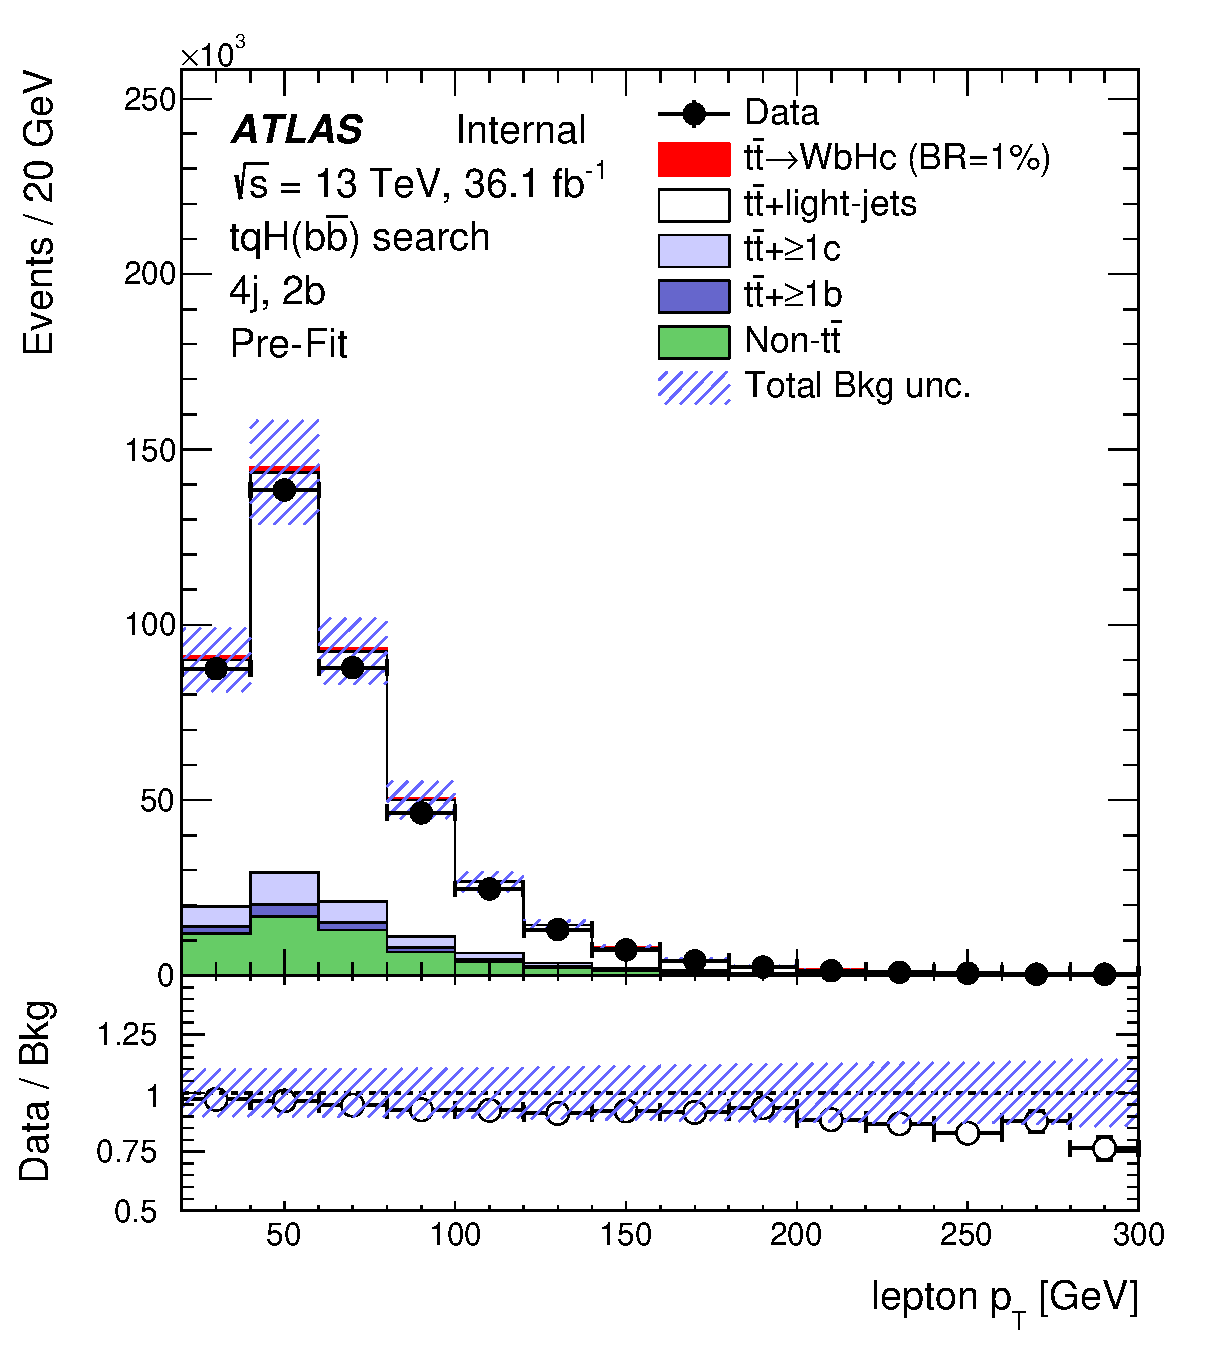
\includegraphics[width=0.40\textwidth]{figures/Hbb/other_variables/c1lep4jex2bex_lep0_pt.eps}}
\subfloat[]{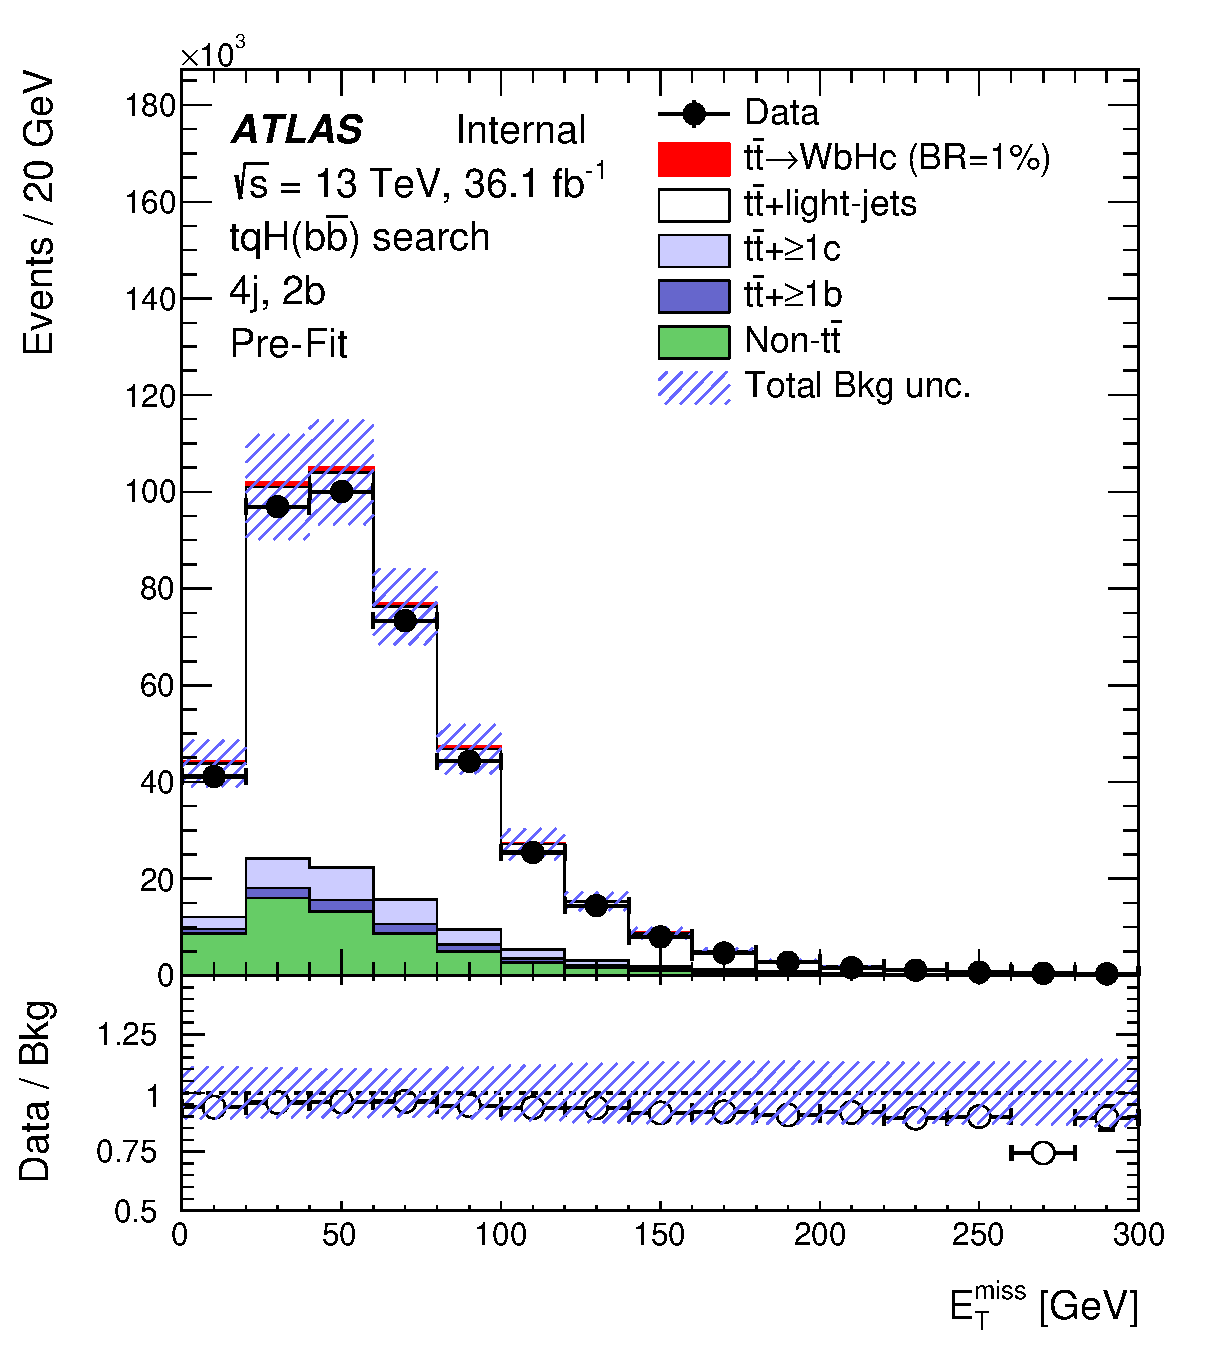
\includegraphics[width=0.40\textwidth]{figures/Hbb/other_variables/c1lep4jex2bex_met.eps}} \\
\subfloat[]{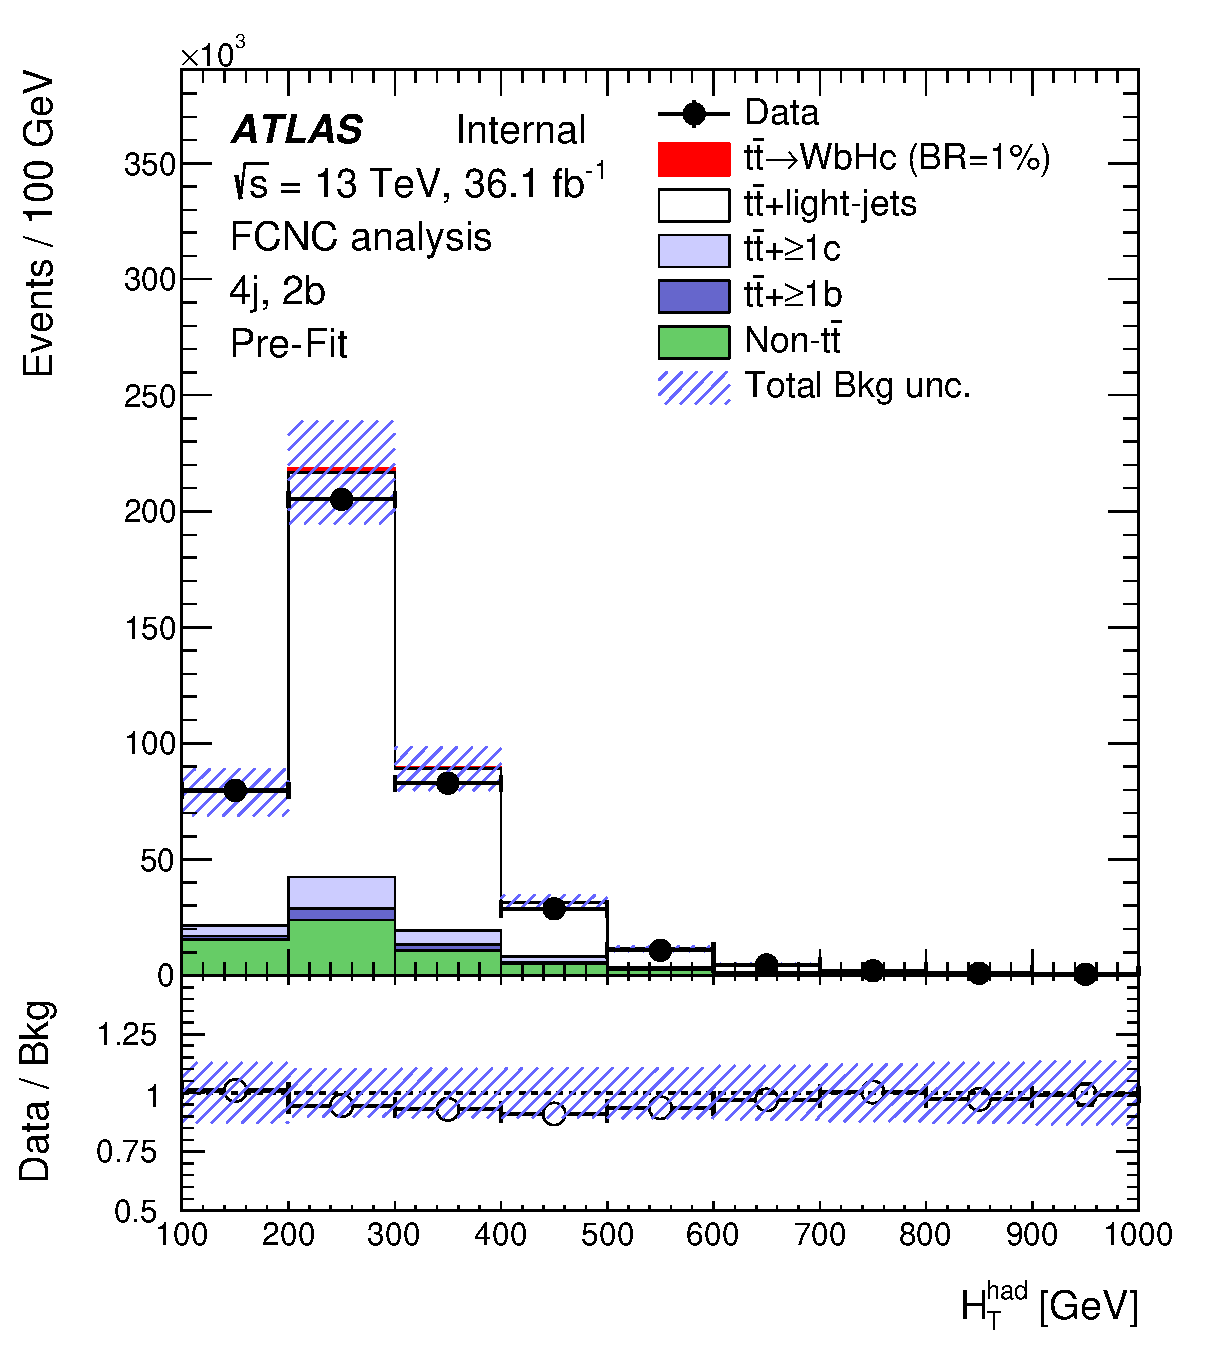
\includegraphics[width=0.40\textwidth]{figures/Hbb/other_variables/c1lep4jex2bex_hthad.eps}} 
\subfloat[]{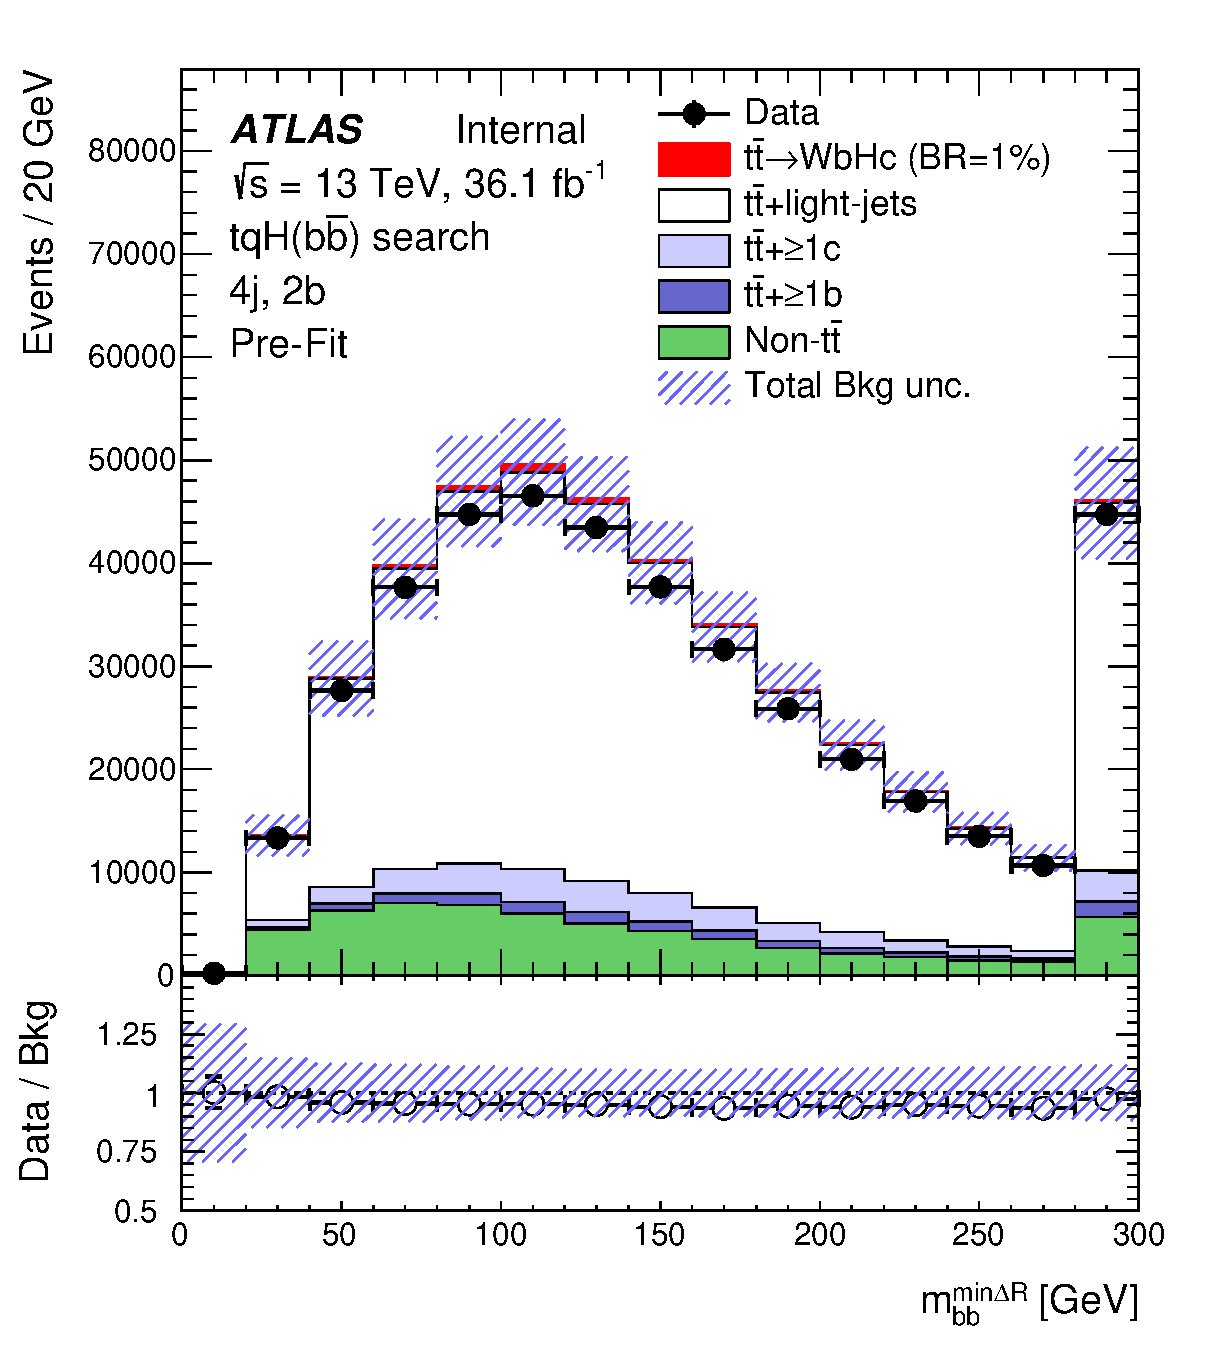
\includegraphics[width=0.40\textwidth]{figures/Hbb/other_variables/c1lep4jex2bex_mbb_mindR.eps}} \\ 
\caption{\small{$\Hbb$ search: Comparison between the data and background prediction for several kinematic 
distributions in the (4j, 2b) region (prior to the application of the cut on the LH discriminant above 0.6) before  the fit to data (``Pre-Fit''). 
The distributions are shown for (a) lepton $\pt$, (b) $\met$, (c) scalar sum of the transverse momenta of 
the jets ($\hthad$), and (d) the invariant mass of the two $b$-tagged jets with lowest 
$\Delta R$ separation ($\mbb$).
The small contributions from $\ttbar V$, $\ttbar H$, single top, $W/Z$+jets, diboson, and multijet backgrounds are combined 
into a single background source referred to as ``Non-$\ttbar$''. 
The expected $\Hc$ signal (solid red) corresponding to $\BR(t\to Hc)=1\%$ is also shown,
added to the background prediction.
The last bin in all figures contains the overflow.
The bottom panel displays the ratio of data to the SM background (``Bkg'') prediction. 
The blue triangles indicate points that are outside the vertical range of the figure. 
The hashed area represents the total uncertainty of the background, excluding the normalisation uncertainty of the $\ttbin$ background, 
which is determined via a likelihood fit to data.}}
\label{fig:Hbb_extravars_4j2b}
\end{center}
\end{figure*}
%%%%%%%%%%%%%%%%%%%%%%%%%%%%%%%%%%%%%%%

%%%%%%%%%%%%%%%%%%%%%%%%%%%%%%%%%%%%%%%%
%\begin{figure*}[htbp]
%\begin{center}
%\subfloat[]{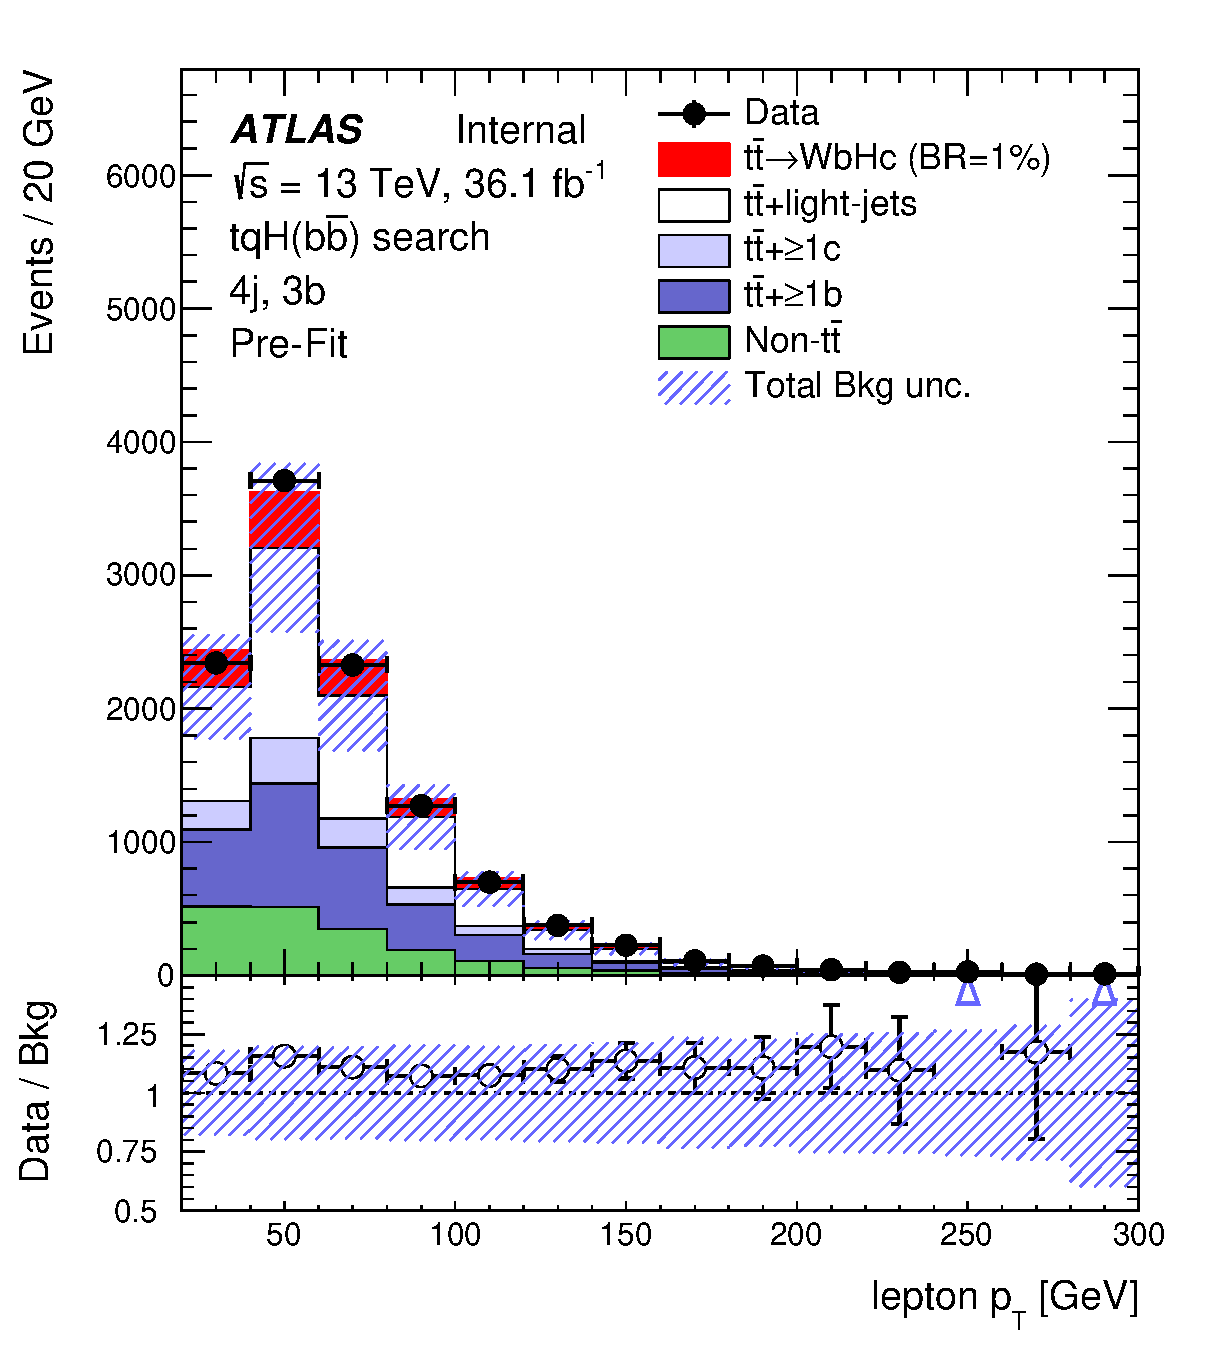
\includegraphics[width=0.40\textwidth]{figures/Hbb/other_variables/c1lep4jex3bex_lep0_pt.eps}}
%\subfloat[]{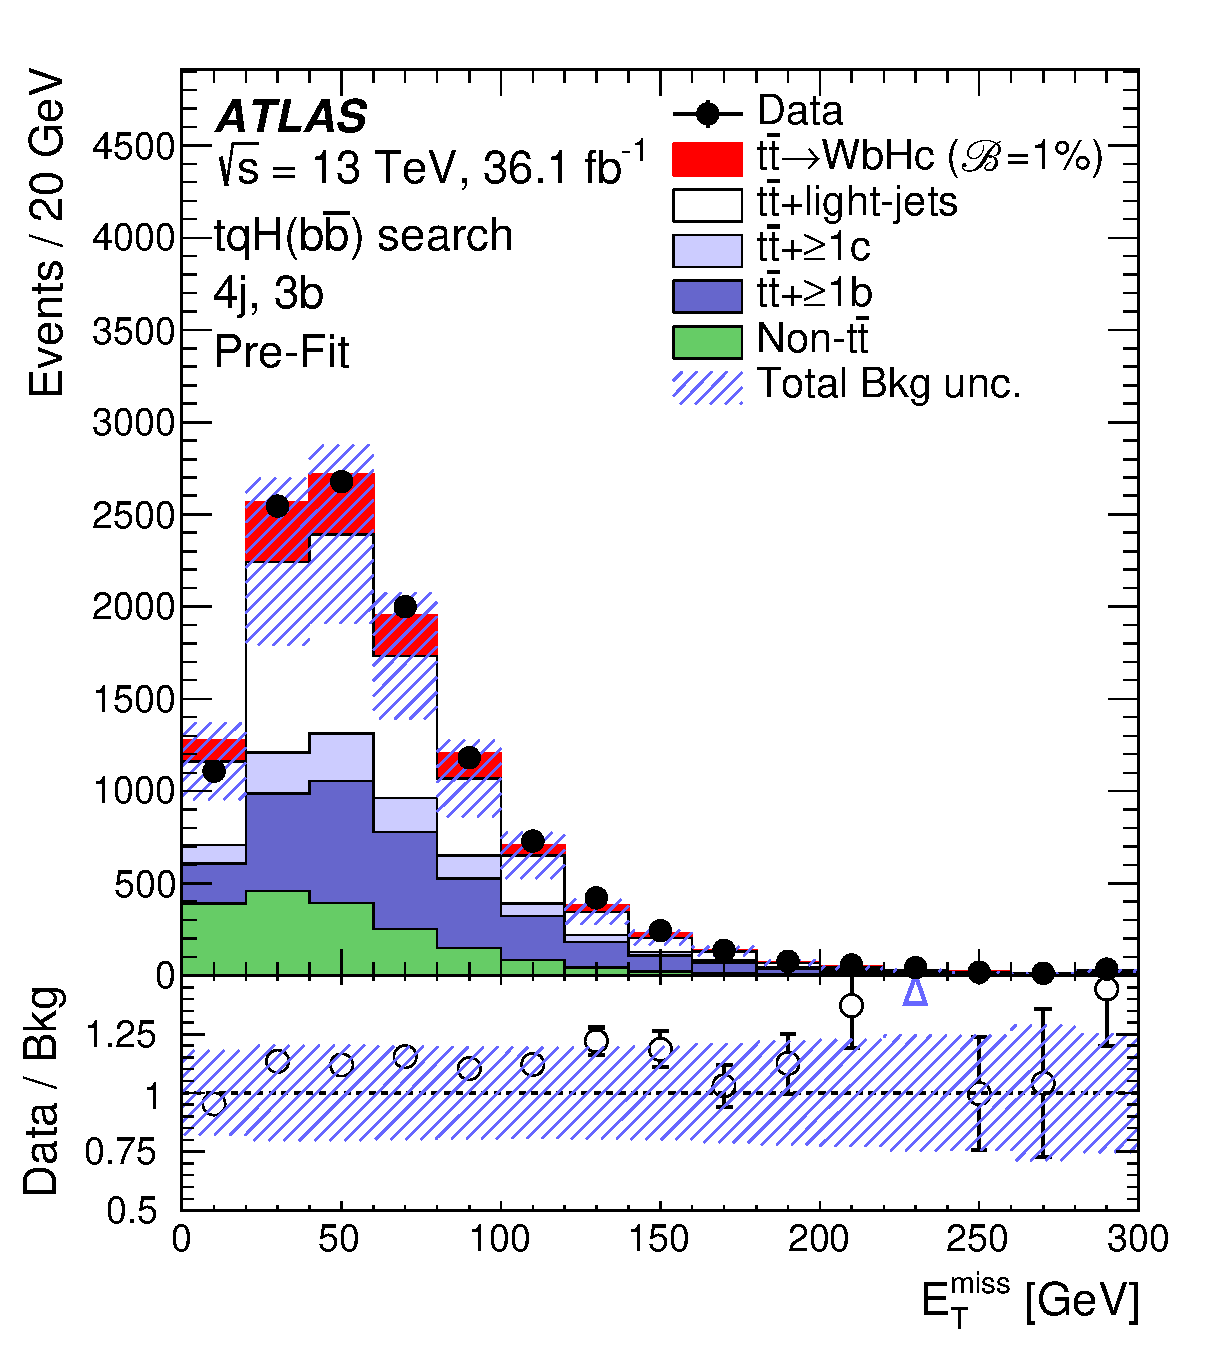
\includegraphics[width=0.40\textwidth]{figures/Hbb/other_variables/c1lep4jex3bex_met.eps}} \\
%\subfloat[]{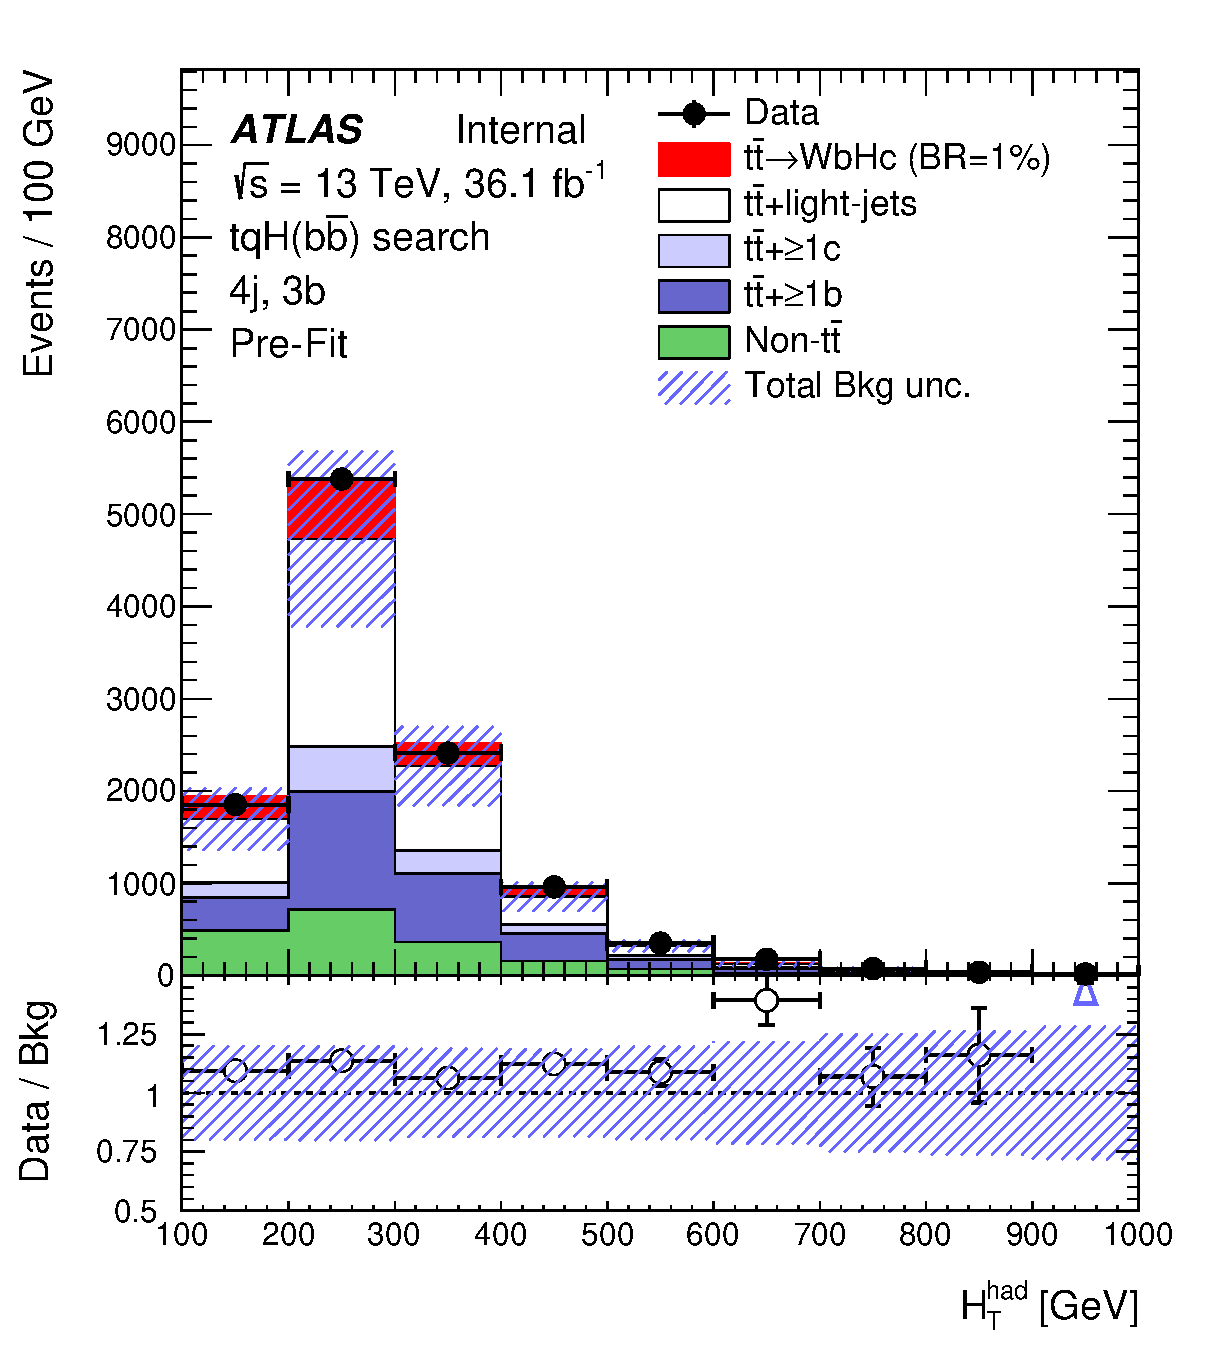
\includegraphics[width=0.40\textwidth]{figures/Hbb/other_variables/c1lep4jex3bex_hthad.eps}} 
%\subfloat[]{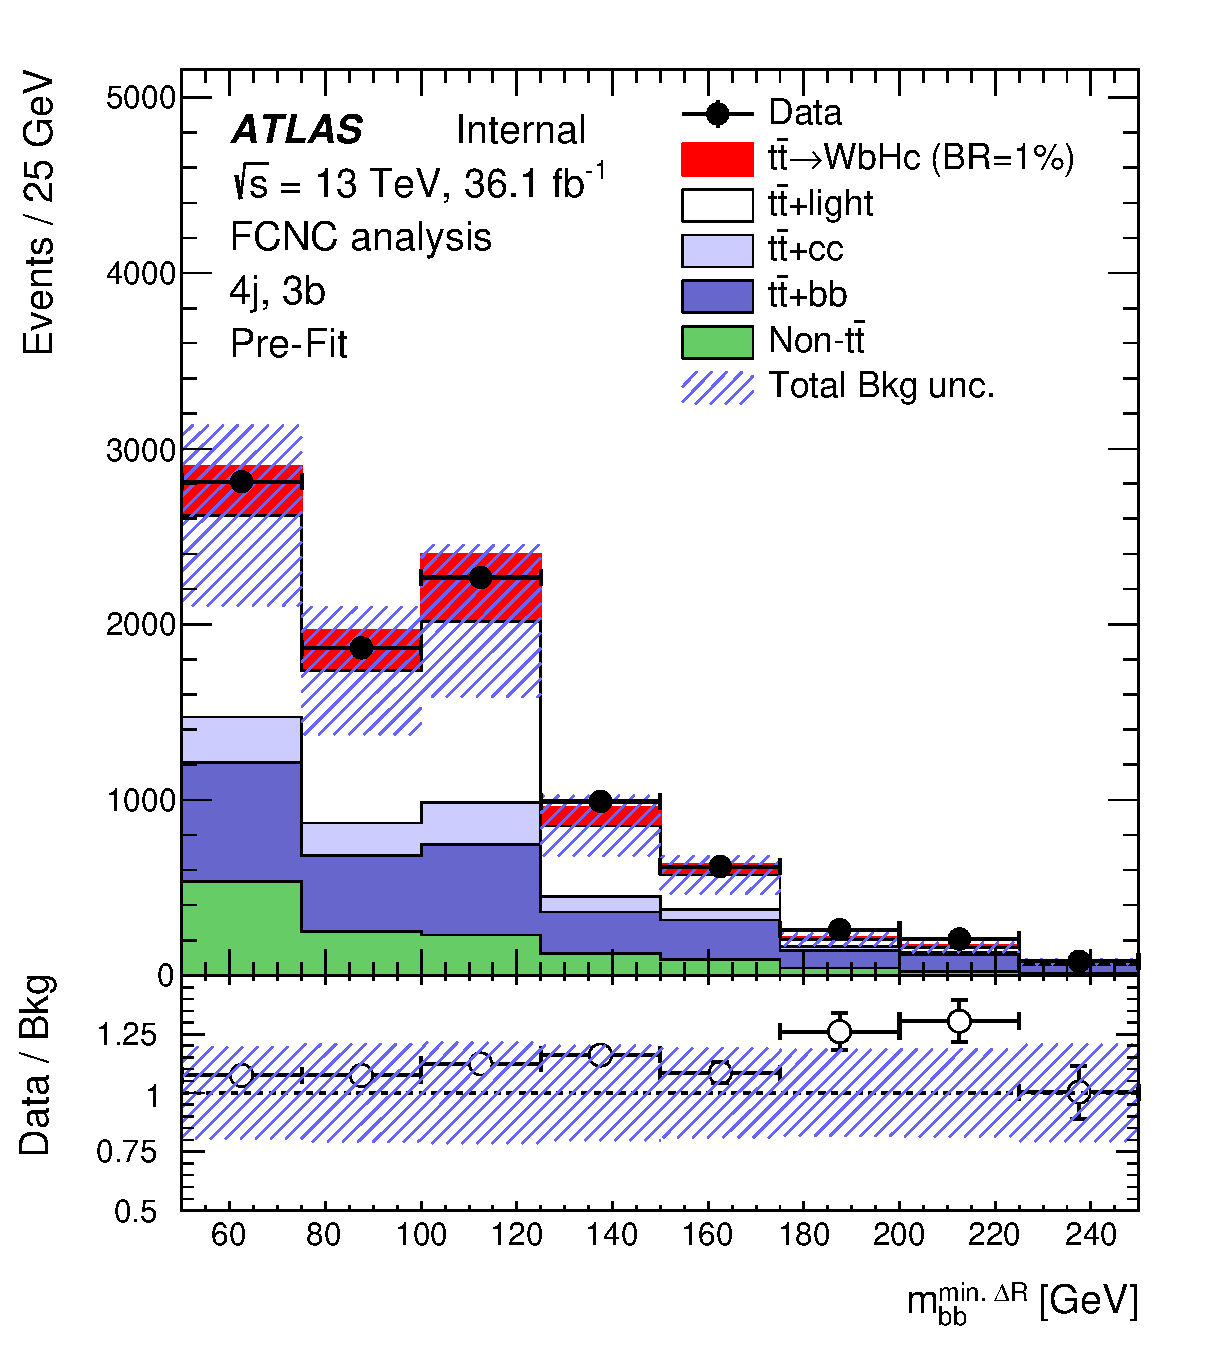
\includegraphics[width=0.40\textwidth]{figures/Hbb/other_variables/c1lep4jex3bex_mbb_mindR.eps}} \\ 
%\caption{\small{$\Hbb$ search: Comparison between the data and background prediction for several kinematic 
%distributions in the (4j, 3b) region before performing the fit to data (``Pre-Fit''). 
%The distributions are shown for (a) lepton $\pt$, (b) $\met$, (c) scalar sum of the transverse momenta of 
%the jets ($\hthad$), and (d) the invariant mass distribution of the two $b$-tagged jets with lowest 
%$\Delta R$ separation ($\mbb$).
%The small contributions from $\ttbar V$, $\ttbar H$, single top, $W/Z$+jets, diboson, and multijet backgrounds are combined 
%into a single background source referred to as ``Non-$\ttbar$''. 
%The expected $\Hc$ signal (solid red) corresponding to $\BR(t\to Hc)=1\%$ is also shown,
%added on top of the background prediction.
%The last bin in all figures contains the overflow.
%The bottom panel displays the ratio of data to the SM background (``Bkg'') prediction. 
%The blue triangles indicate points that are outside the vertical range of the figure. 
%The hashed area represents the total uncertainty on the background, excluding the normalisation uncertainty of the $\ttbin$ background, 
%which is determined via a likelihood fit to data.}}
%\label{fig:Hbb_extravars_4j3b}
%\end{center}
%\end{figure*}
%%%%%%%%%%%%%%%%%%%%%%%%%%%%%%%%%%%%%%%%

%%%%%%%%%%%%%%%%%%%%%%%%%%%%%%%%%%%%%%%
\begin{figure*}[htbp]
\begin{center}
\subfloat[]{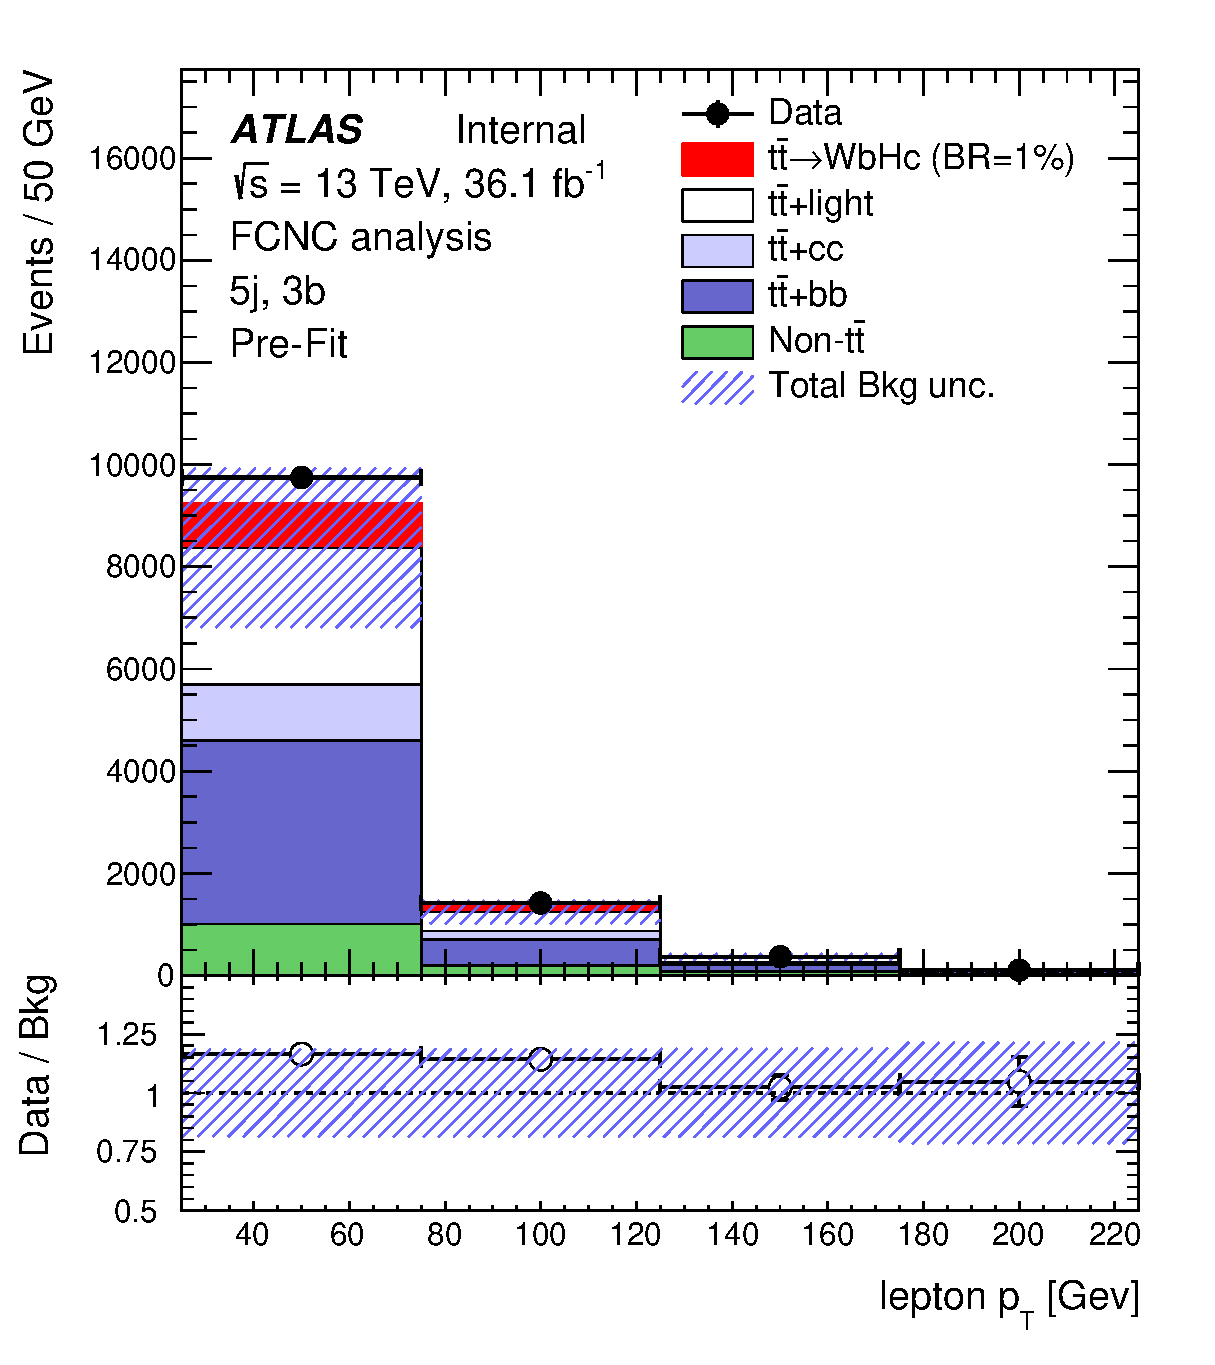
\includegraphics[width=0.40\textwidth]{figures/Hbb/other_variables/c1lep5jex3bex_lep0_pt.eps}}
\subfloat[]{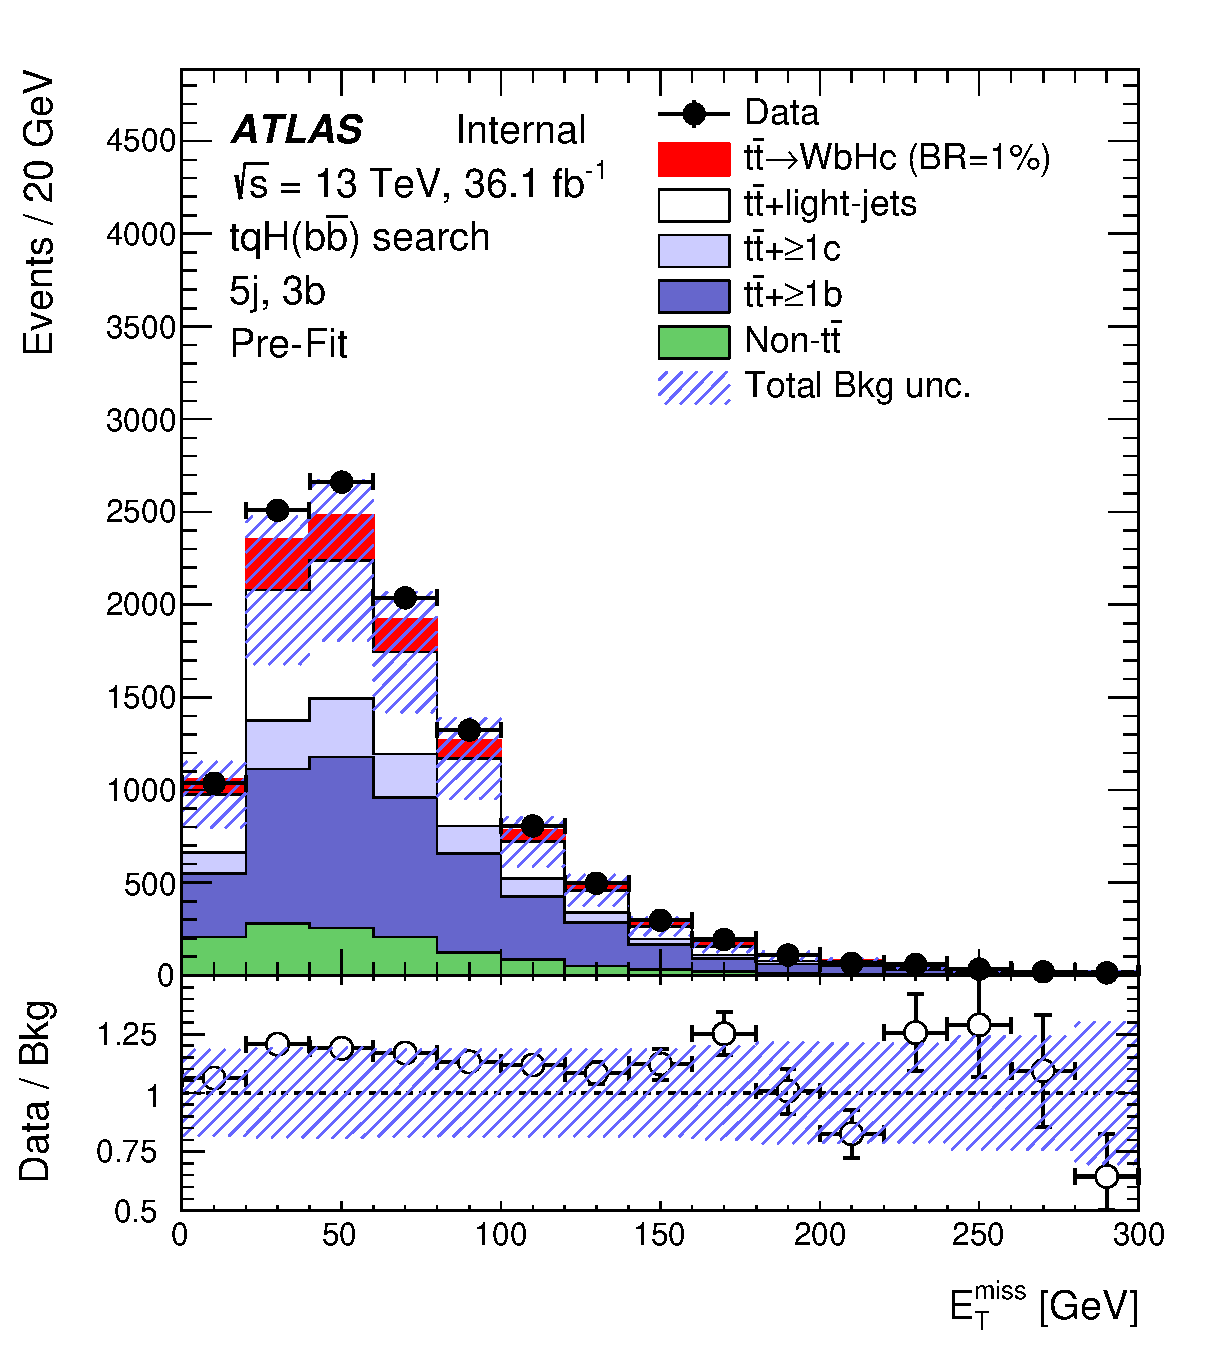
\includegraphics[width=0.40\textwidth]{figures/Hbb/other_variables/c1lep5jex3bex_met.eps}} \\
\subfloat[]{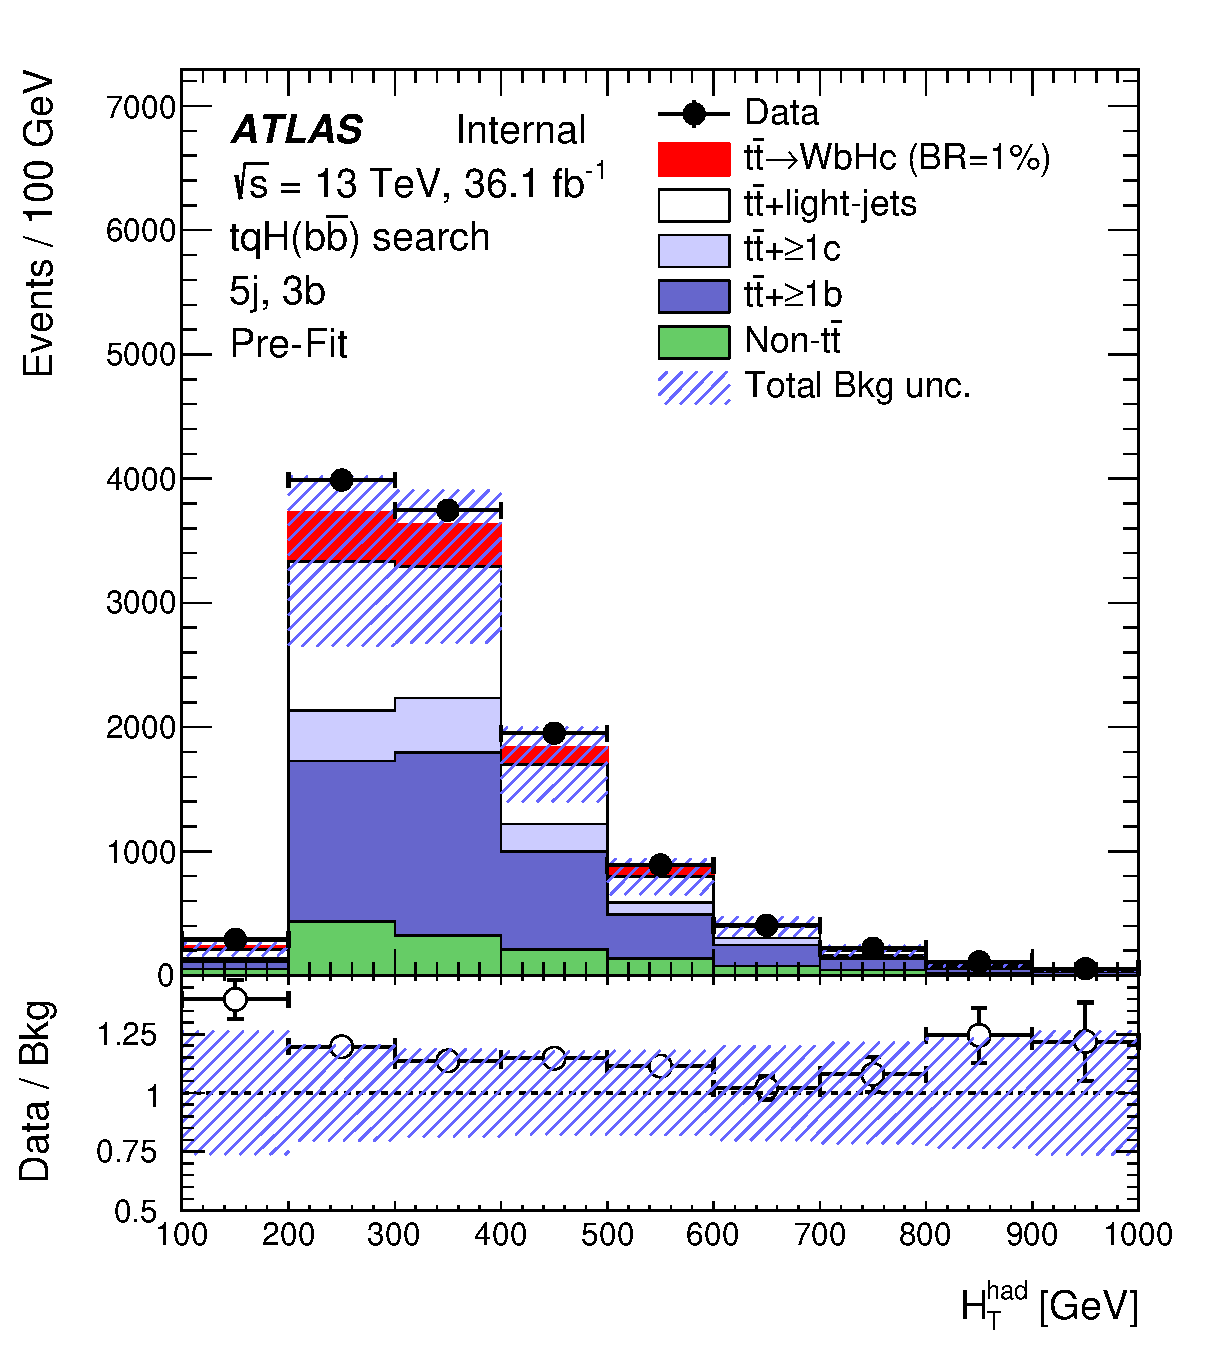
\includegraphics[width=0.40\textwidth]{figures/Hbb/other_variables/c1lep5jex3bex_hthad.eps}} 
\subfloat[]{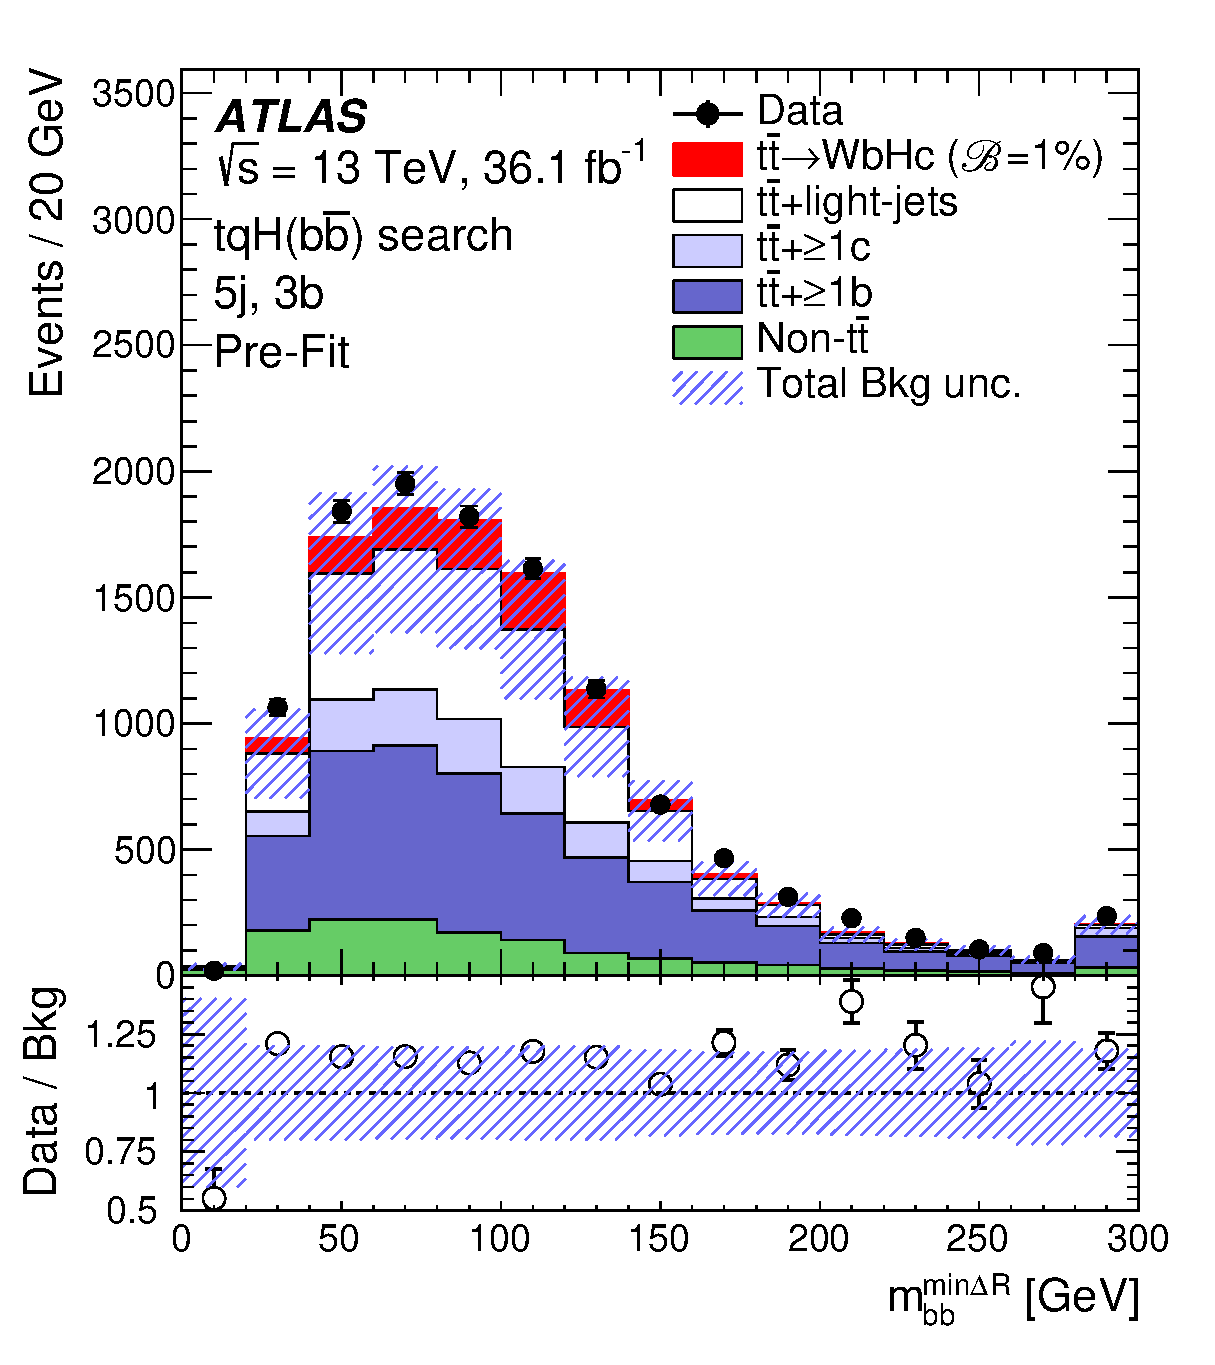
\includegraphics[width=0.40\textwidth]{figures/Hbb/other_variables/c1lep5jex3bex_mbb_mindR.eps}} \\ 
\caption{\small{$\Hbb$ search: Comparison between the data and background prediction for several kinematic 
distributions in the (5j, 3b) region before the fit to data (``Pre-Fit''). 
The distributions are shown for (a) lepton $\pt$, (b) $\met$, (c) scalar sum of the transverse momenta of 
the jets ($\hthad$), and (d) the invariant mass of the two $b$-tagged jets with lowest 
$\Delta R$ separation ($\mbb$).
The small contributions from $\ttbar V$, $\ttbar H$, single top, $W/Z$+jets, diboson, and multijet backgrounds are combined 
into a single background source referred to as ``Non-$\ttbar$''. 
The expected $\Hc$ signal (solid red) corresponding to $\BR(t\to Hc)=1\%$ is also shown,
added to the background prediction.
The last bin in all figures contains the overflow.
The bottom panel displays the ratio of data to the SM background (``Bkg'') prediction. 
The blue triangles indicate points that are outside the vertical range of the figure. 
The hashed area represents the total uncertainty of the background, excluding the normalisation uncertainty of the $\ttbin$ background, 
which is determined via a likelihood fit to data.}}
\label{fig:Hbb_extravars_5j3b}
\end{center}
\end{figure*}
%%%%%%%%%%%%%%%%%%%%%%%%%%%%%%%%%%%%%%%

%%%%%%%%%%%%%%%%%%%%%%%%%%%%%%%%%%%%%%%
\begin{figure*}[t]
\begin{center}
\subfloat[]{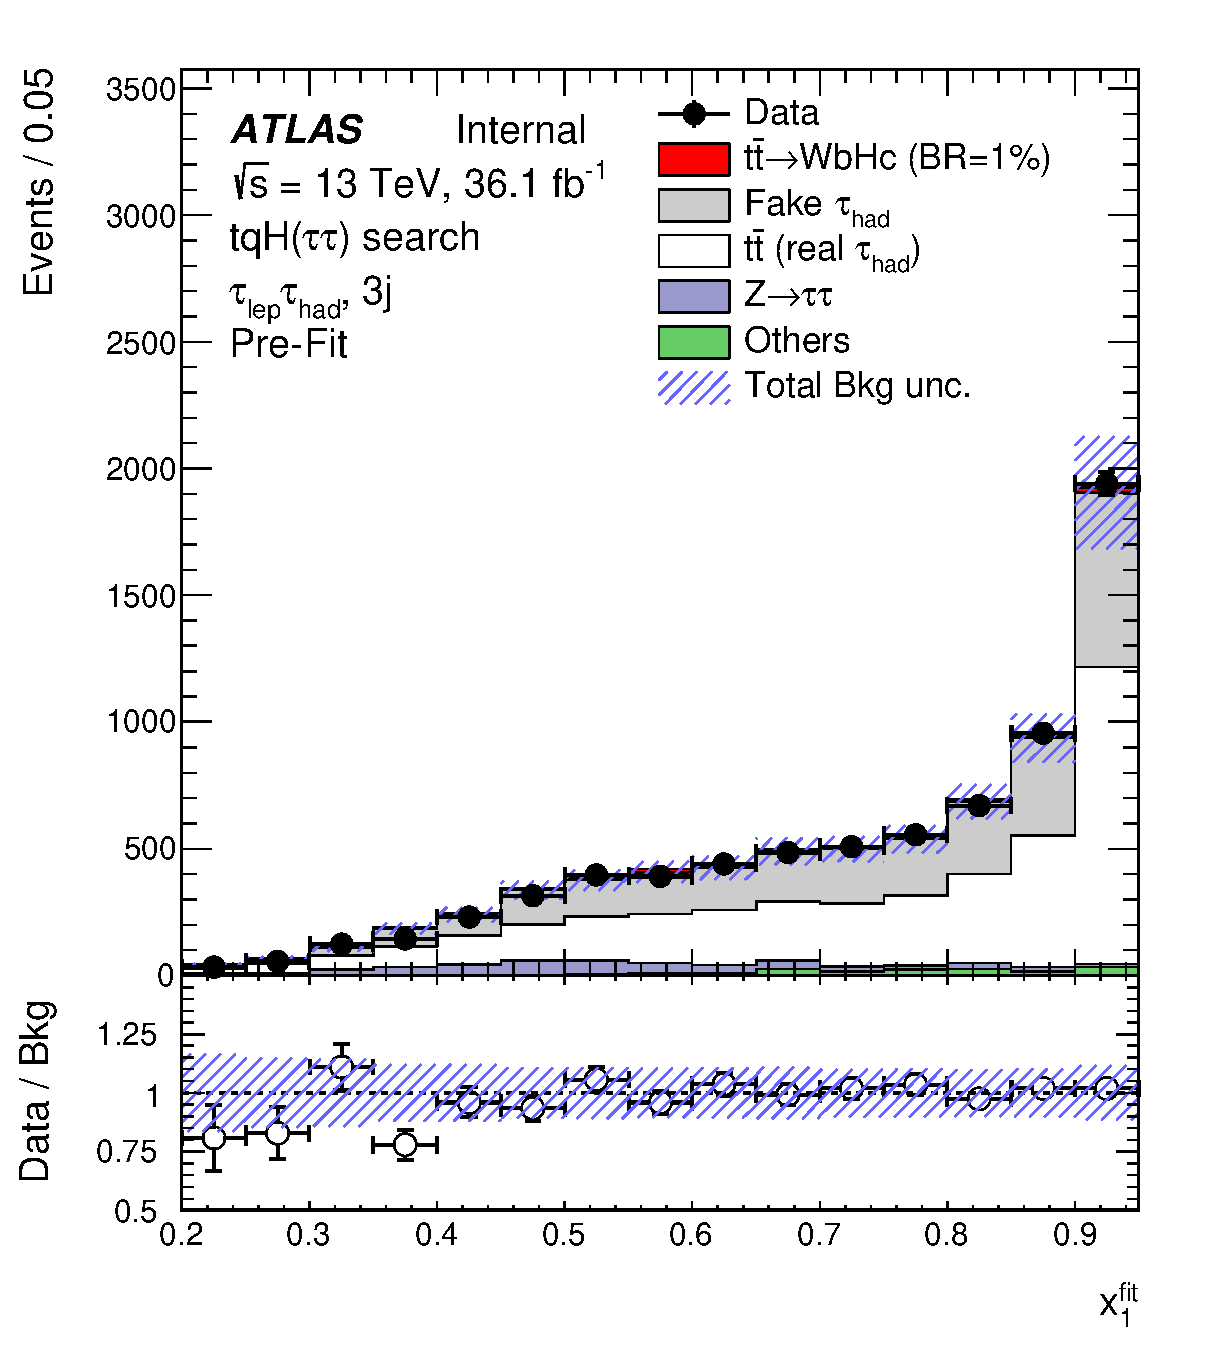
\includegraphics[width=0.40\textwidth]{figures/Htautau/control_plots/x1_fit_lephad_3j_FR.eps}}
\subfloat[]{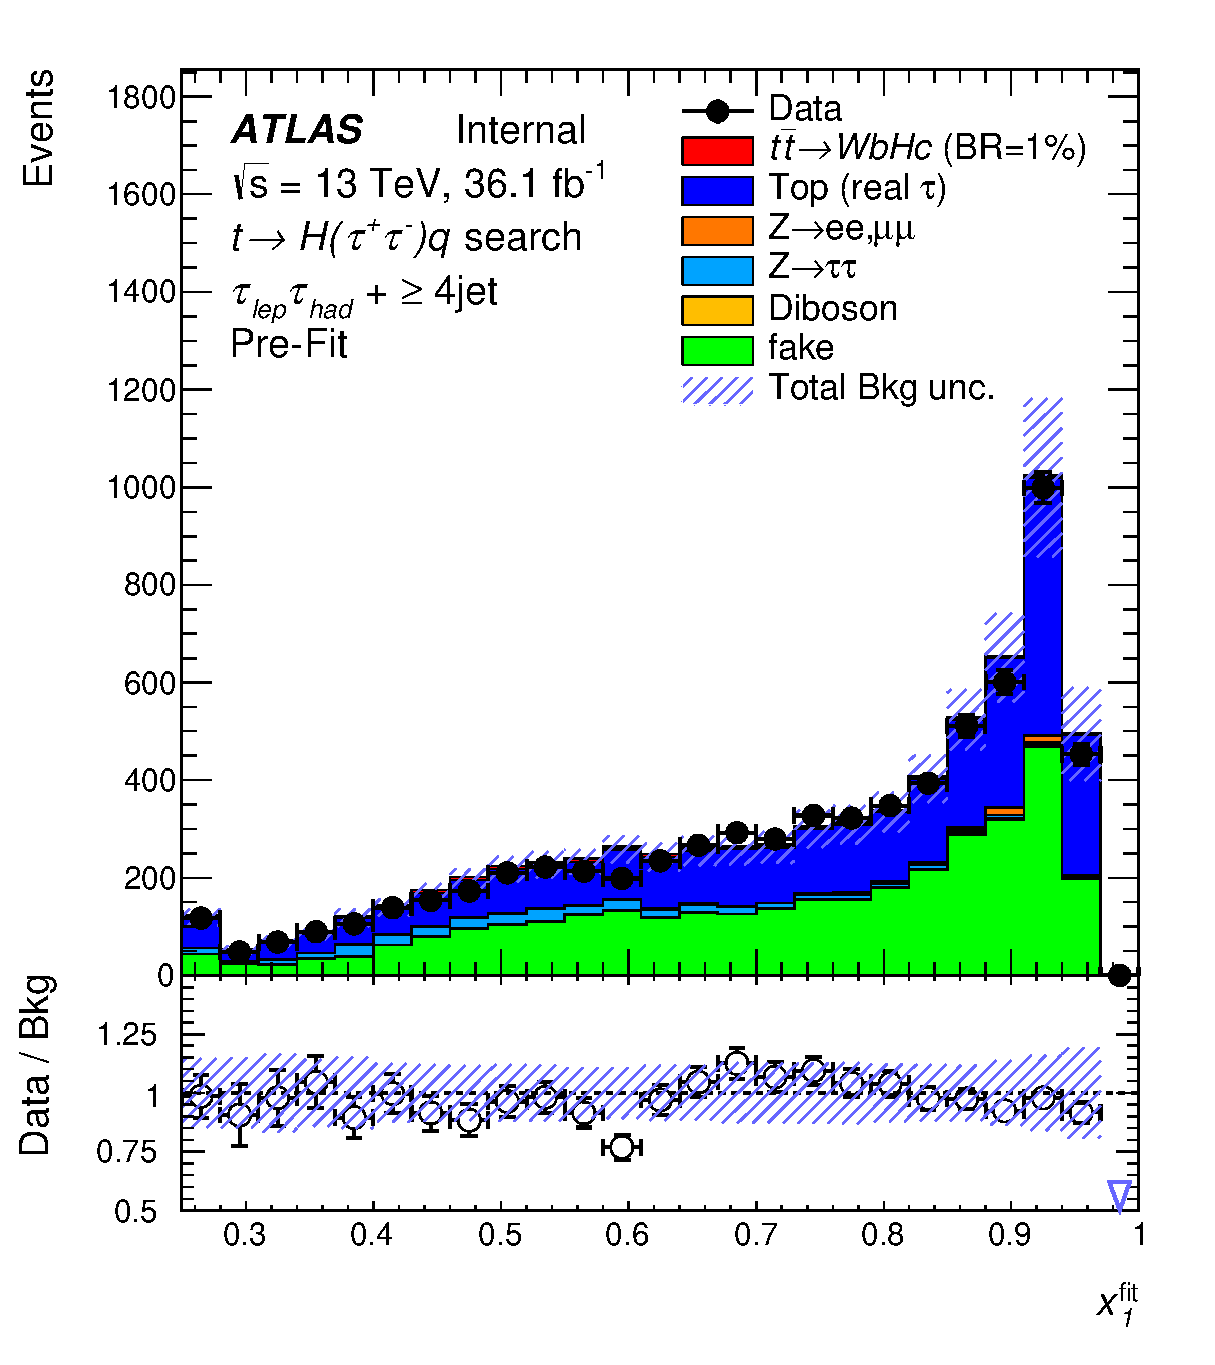
\includegraphics[width=0.40\textwidth]{figures/Htautau/control_plots/x1_fit_lephad_4j_FR.eps}} \\
\subfloat[]{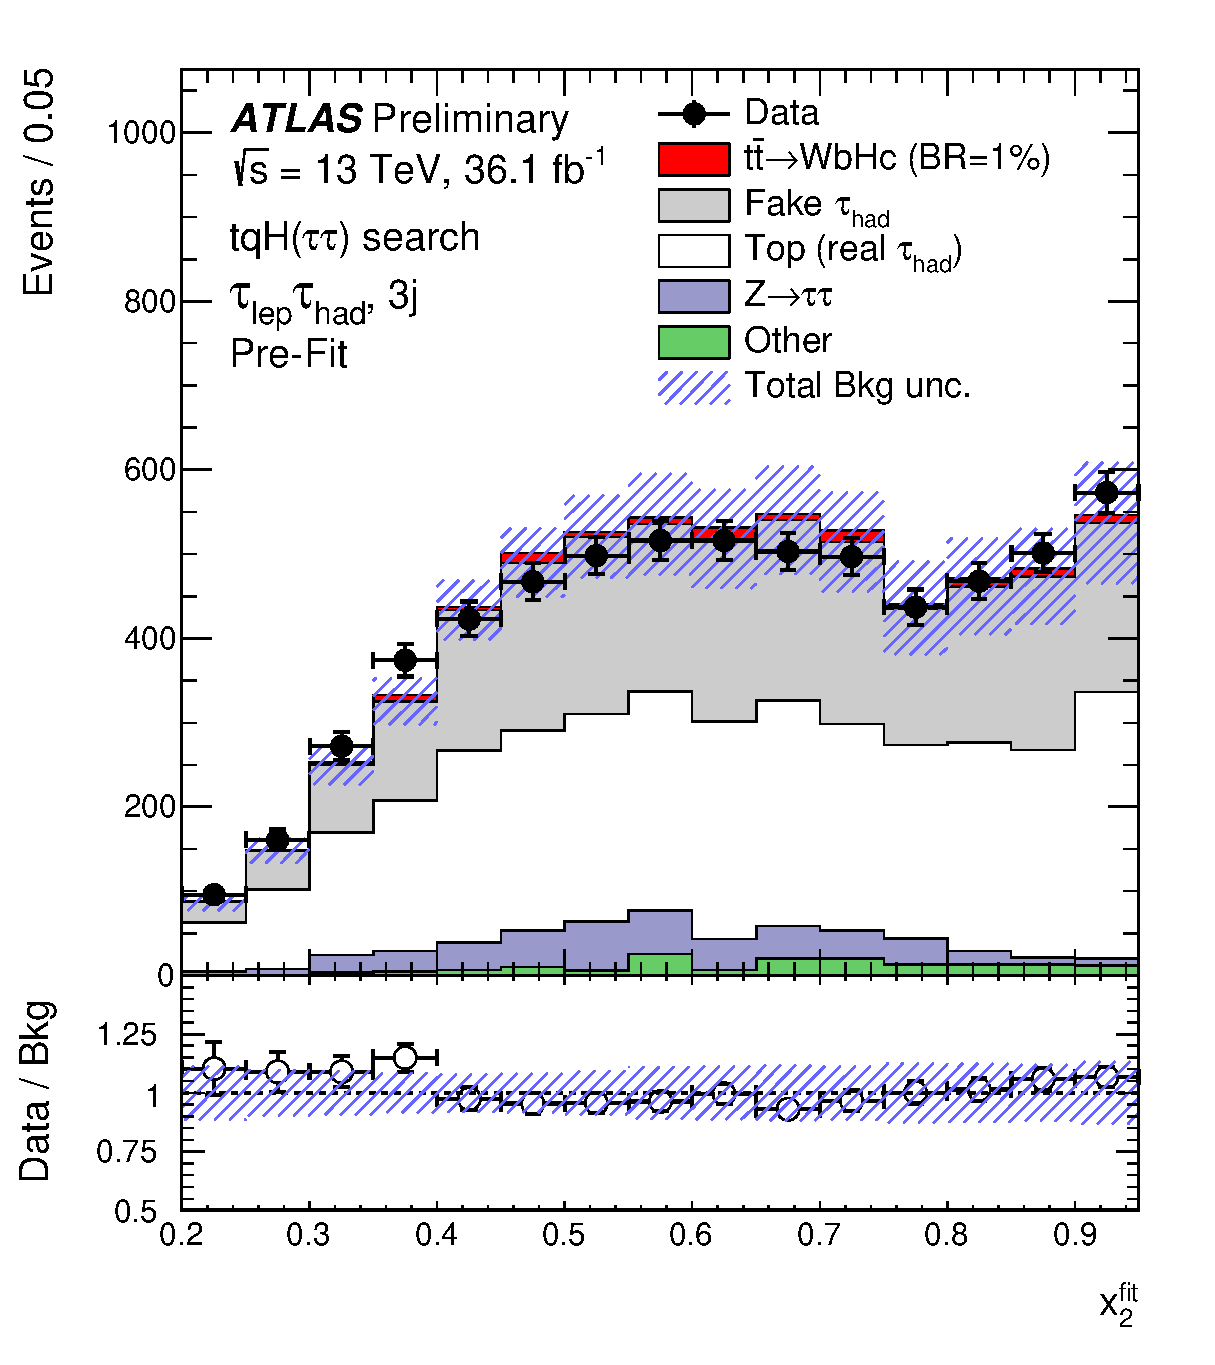
\includegraphics[width=0.40\textwidth]{figures/Htautau/control_plots/x2_fit_lephad_3j_FR.eps}}
\subfloat[]{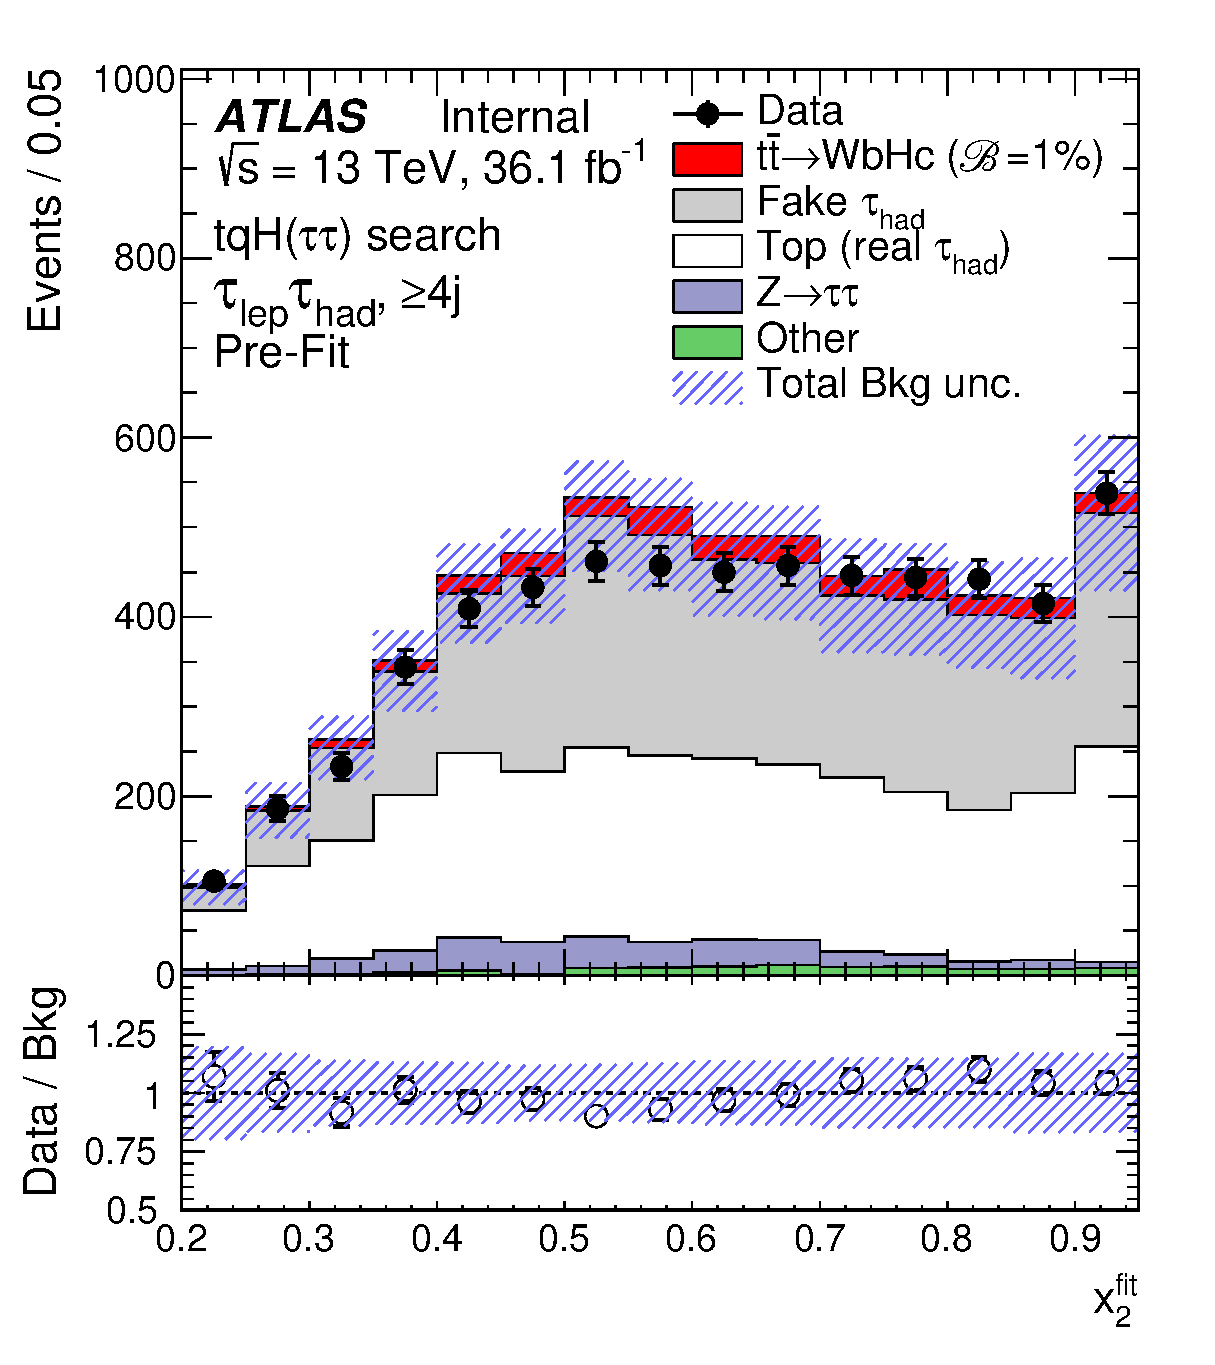
\includegraphics[width=0.40\textwidth]{figures/Htautau/control_plots/x2_fit_lephad_4j_FR.eps}} \\
\caption{$\Htautau$ search: Comparison between the data and background prediction for the distribution of some of the most
discriminating BDT input variables in the $\lephad$ channel before the fit to data (``Pre-Fit''). The distributions are shown for
$x_{1}^{\text{fit}}$ in (a) the ($\lephad$, 3j) region and (b) the ($\lephad$, $\geq$4j) region, and for
$x_{2}^{\text{fit}}$ in (c) the ($\lephad$, 3j)  region and (d) the ($\lephad$, $\geq$4j) region.
The contributions with real $\had$ candidates from $\ttbar$,  $\ttbar V$, $\ttbar H$, and single top backgrounds are combined into
a single background source referred to as ``Top (real $\had$)", whereas the small contributions from 
$Z\to \ell^+\ell^-$ ($\ell = e, \mu$) and diboson backgrounds are combined into ``Other''. 
The expected $\Hc$ signal (solid red) corresponding to $\BR(t\to Hc)=1\%$ is also shown,
added to the background prediction.
%The first and the last bins in all figures contain the underflow and overflow respectively.
The bottom panel displays the ratio of data to the SM background (``Bkg'') prediction.
The hashed area represents the total uncertainty of the background, excluding the normalisation uncertainty of the fake $\had$ background, 
which is determined via a likelihood fit to data.}
\label{fig:BDT_inputs_lephad_2}
\end{center}
\end{figure*}
%%%%%%%%%%%%%%%%%%%%%%%%%%%%%%%%%%%%%%%


%%%%%%%%%%%%%%%%%%%%%%%%%%%%%%%%%%%%%%%
\begin{figure*}[t]
\begin{center}
\subfloat[]{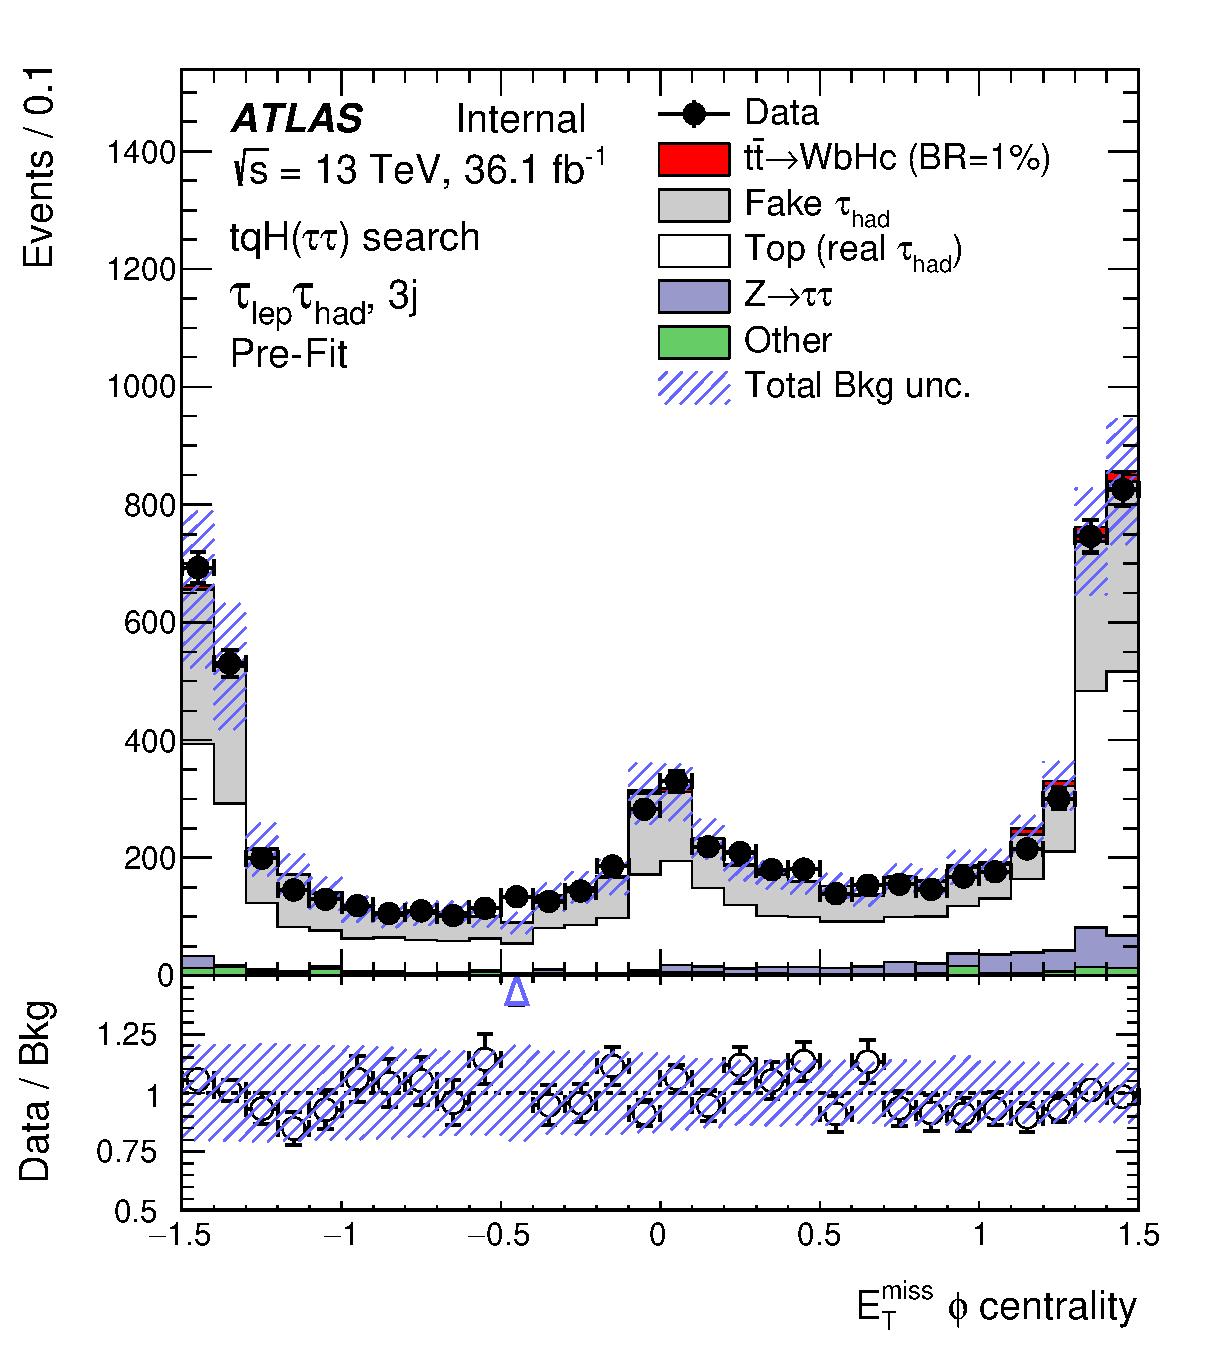
\includegraphics[width=0.40\textwidth]{figures/Htautau/control_plots/met_centrality_lephad_3j_FR.eps}}
\subfloat[]{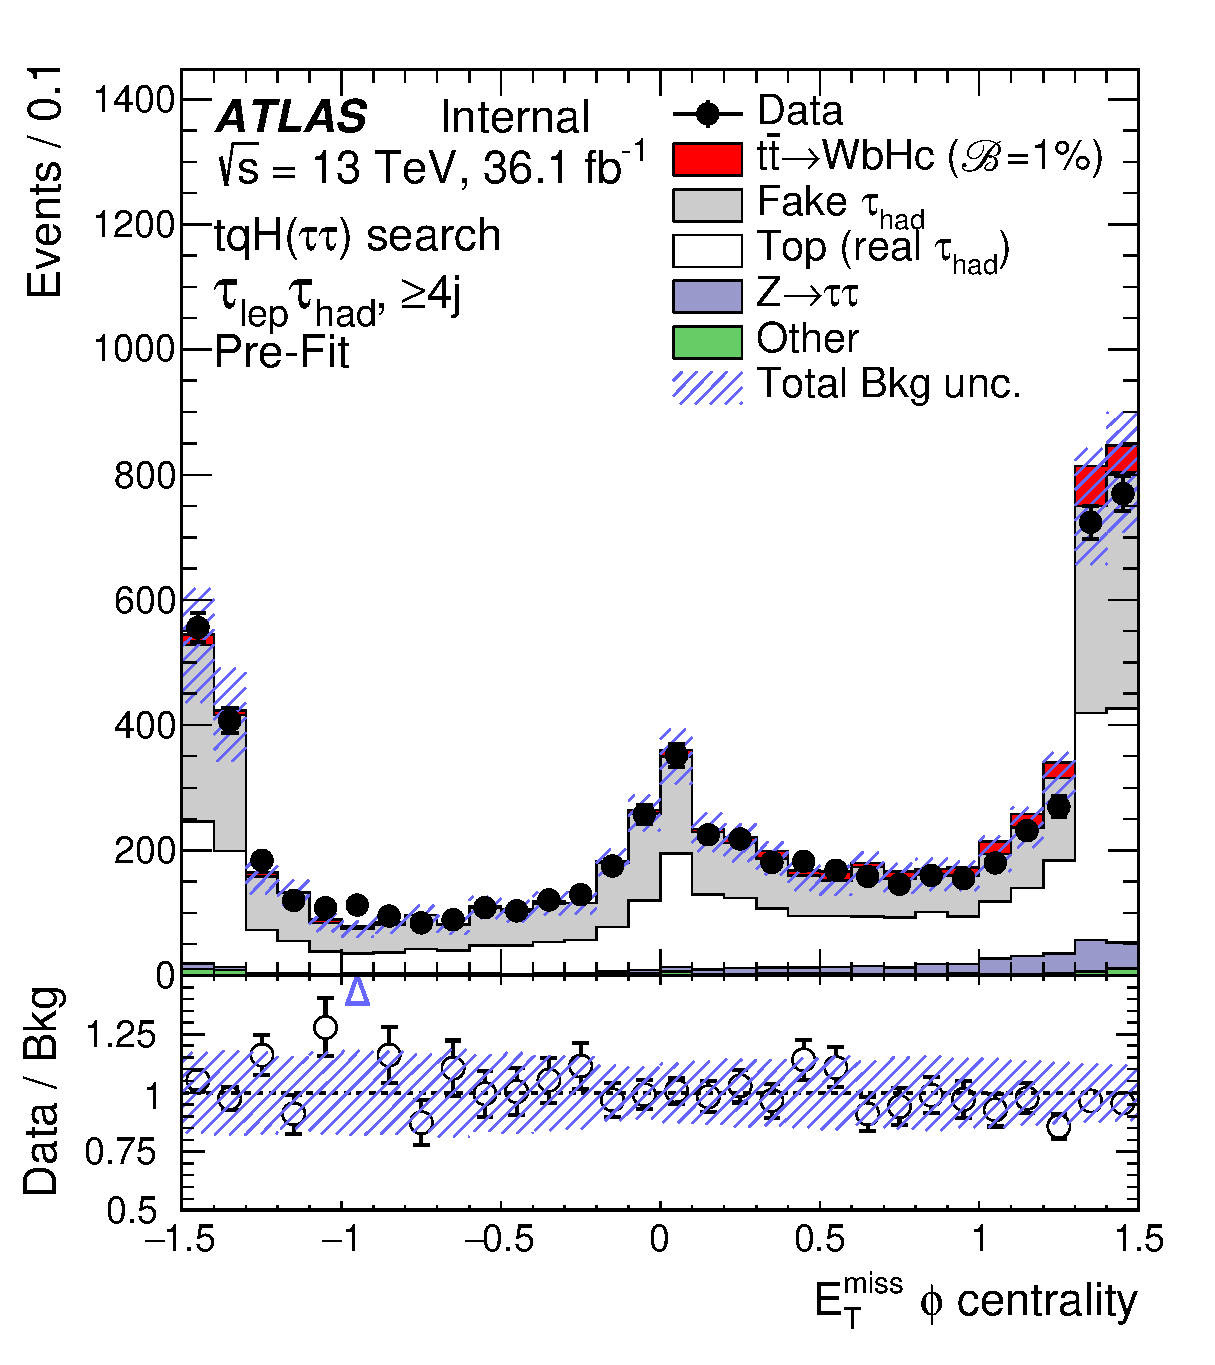
\includegraphics[width=0.40\textwidth]{figures/Htautau/control_plots/met_centrality_lephad_4j_FR.eps}} \\
\subfloat[]{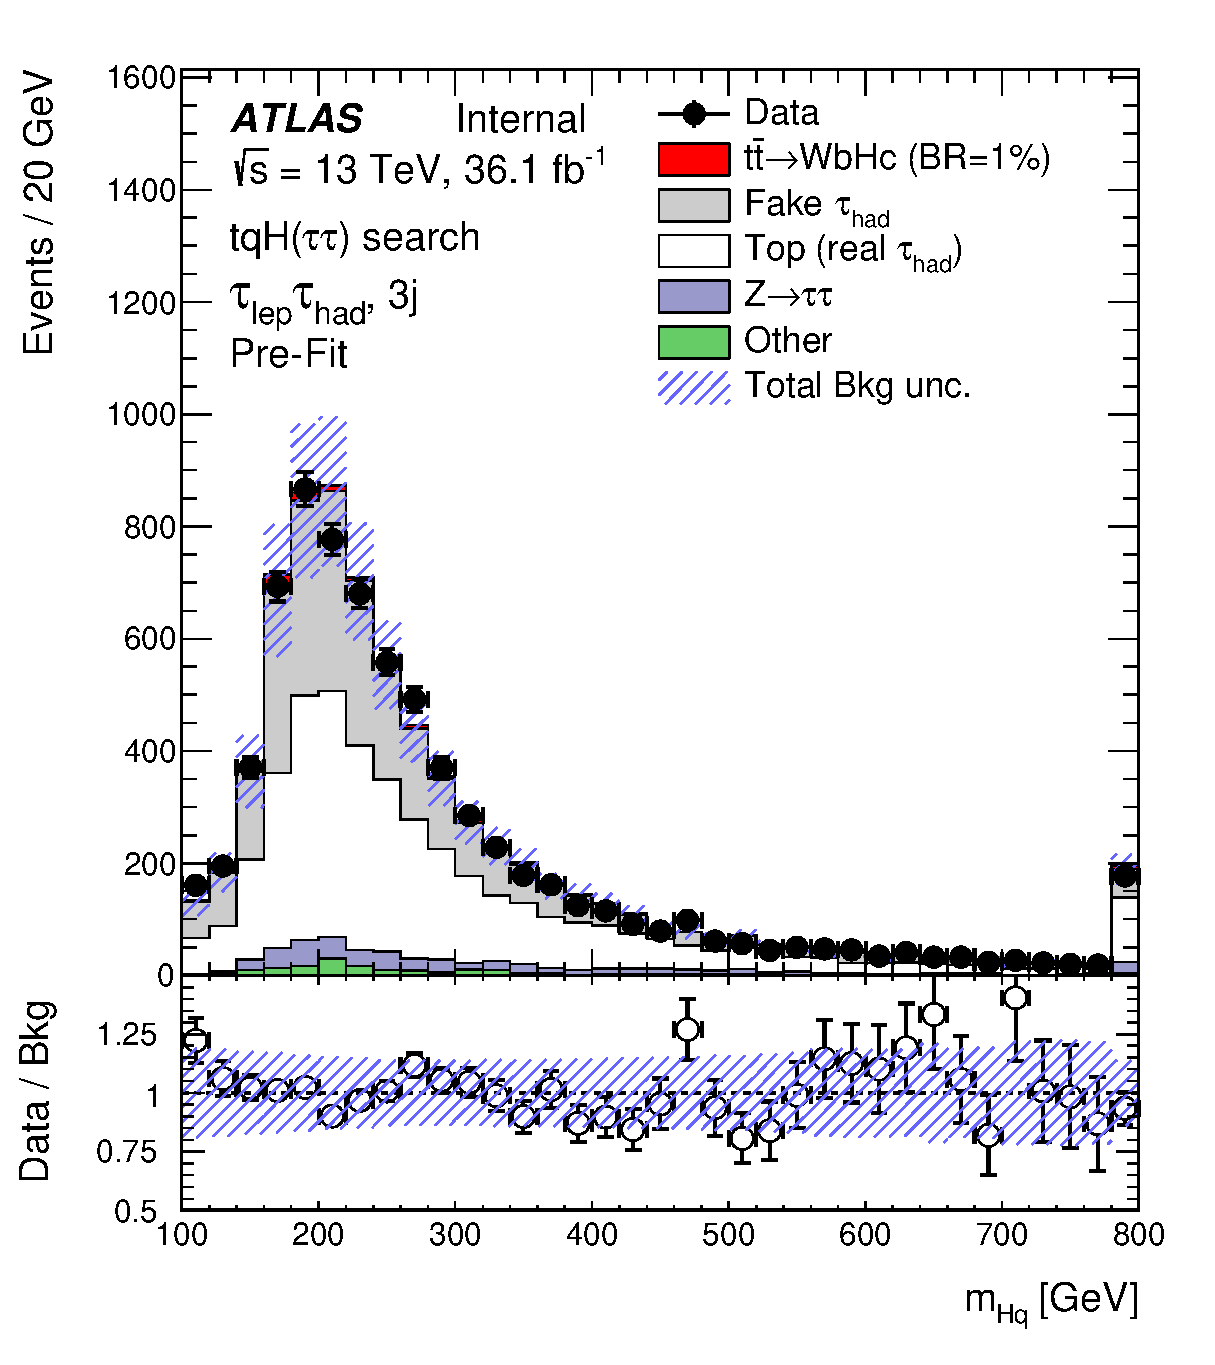
\includegraphics[width=0.40\textwidth]{figures/Htautau/control_plots/mtop_thc_lephad_3j_FR.eps}}
\subfloat[]{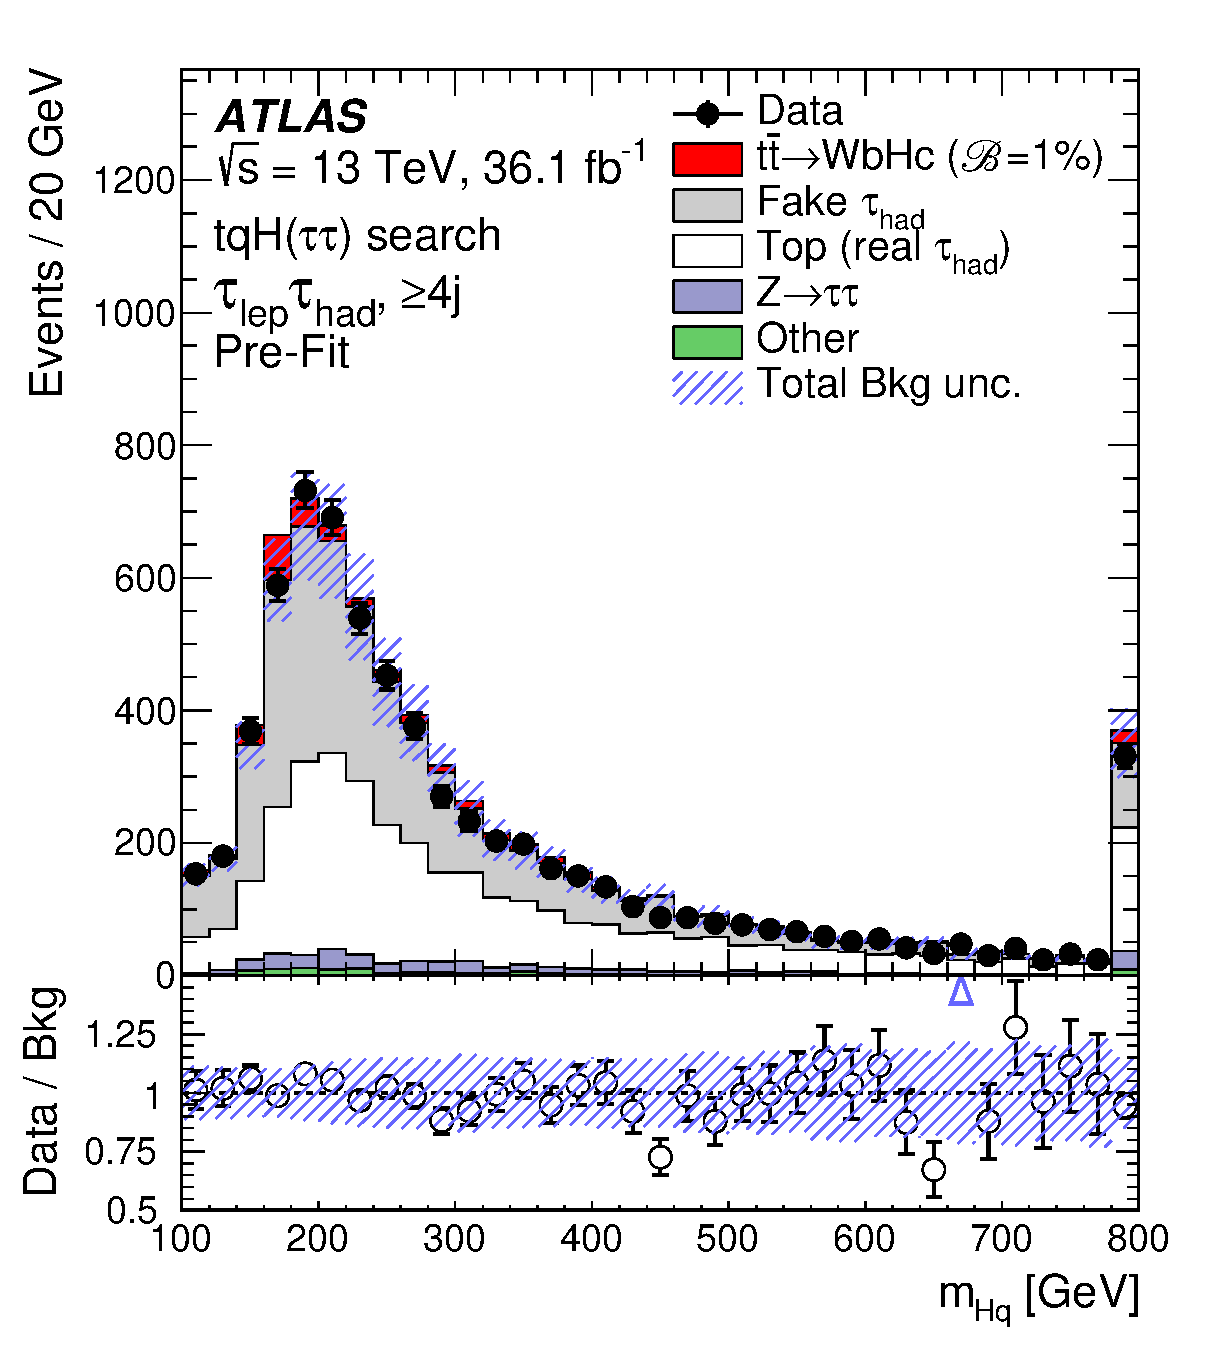
\includegraphics[width=0.40\textwidth]{figures/Htautau/control_plots/mtop_thc_lephad_4j_FR.eps}} \\
\caption{$\Htautau$ search: Comparison between the data and background prediction for the distribution of some of the most
discriminating BDT input variables in the $\lephad$ channel before the fit to data (``Pre-Fit''). The distributions are shown for
$\met$ $\phi$ centrality in (a) the ($\lephad$, 3j) region and (b) the ($\lephad$, $\geq$4j) region, and for
$m_{Hq}$ in (c) the ($\lephad$, 3j)  region and (d) the ($\lephad$, $\geq$4j) region.
The contributions with real $\had$ candidates from $\ttbar$,  $\ttbar V$, $\ttbar H$, and single top backgrounds are combined into
a single background source referred to as ``Top (real $\had$)", whereas the small contributions from 
$Z\to \ell^+\ell^-$ ($\ell = e, \mu$) and diboson backgrounds are combined into ``Other''. 
The expected $\Hc$ signal (solid red) corresponding to $\BR(t\to Hc)=1\%$ is also shown,
added to the background prediction.
%The first and the last bins in all figures contain the underflow and overflow respectively.
The bottom panel displays the ratio of data to the SM background (``Bkg'') prediction.
The hashed area represents the total uncertainty of the background, excluding the normalisation uncertainty of the fake $\had$ background, 
which is determined via a likelihood fit to data.}
\label{fig:BDT_inputs_lephad_3}
\end{center}
\end{figure*}
%%%%%%%%%%%%%%%%%%%%%%%%%%%%%%%%%%%%%%%


%%%%%%%%%%%%%%%%%%%%%%%%%%%%%%%%%%%%%%%
\begin{figure*}[t]
\begin{center}
\subfloat[]{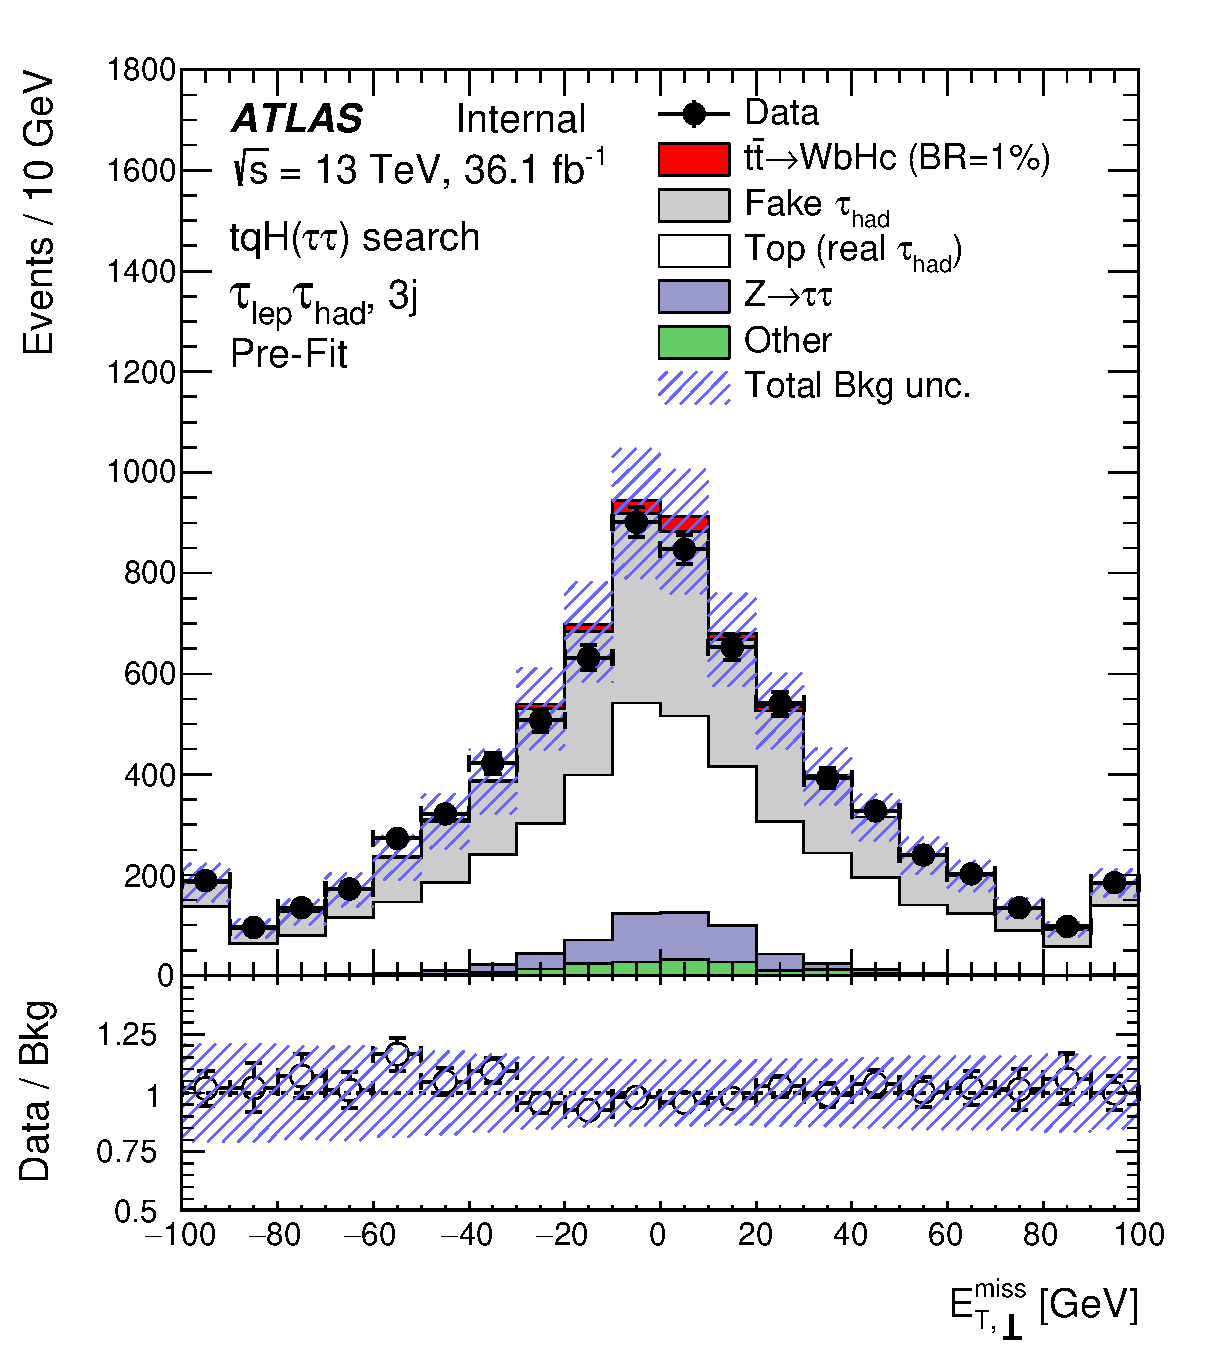
\includegraphics[width=0.40\textwidth]{figures/Htautau/control_plots/MET_perp_lephad_3j_FR.eps}}
\subfloat[]{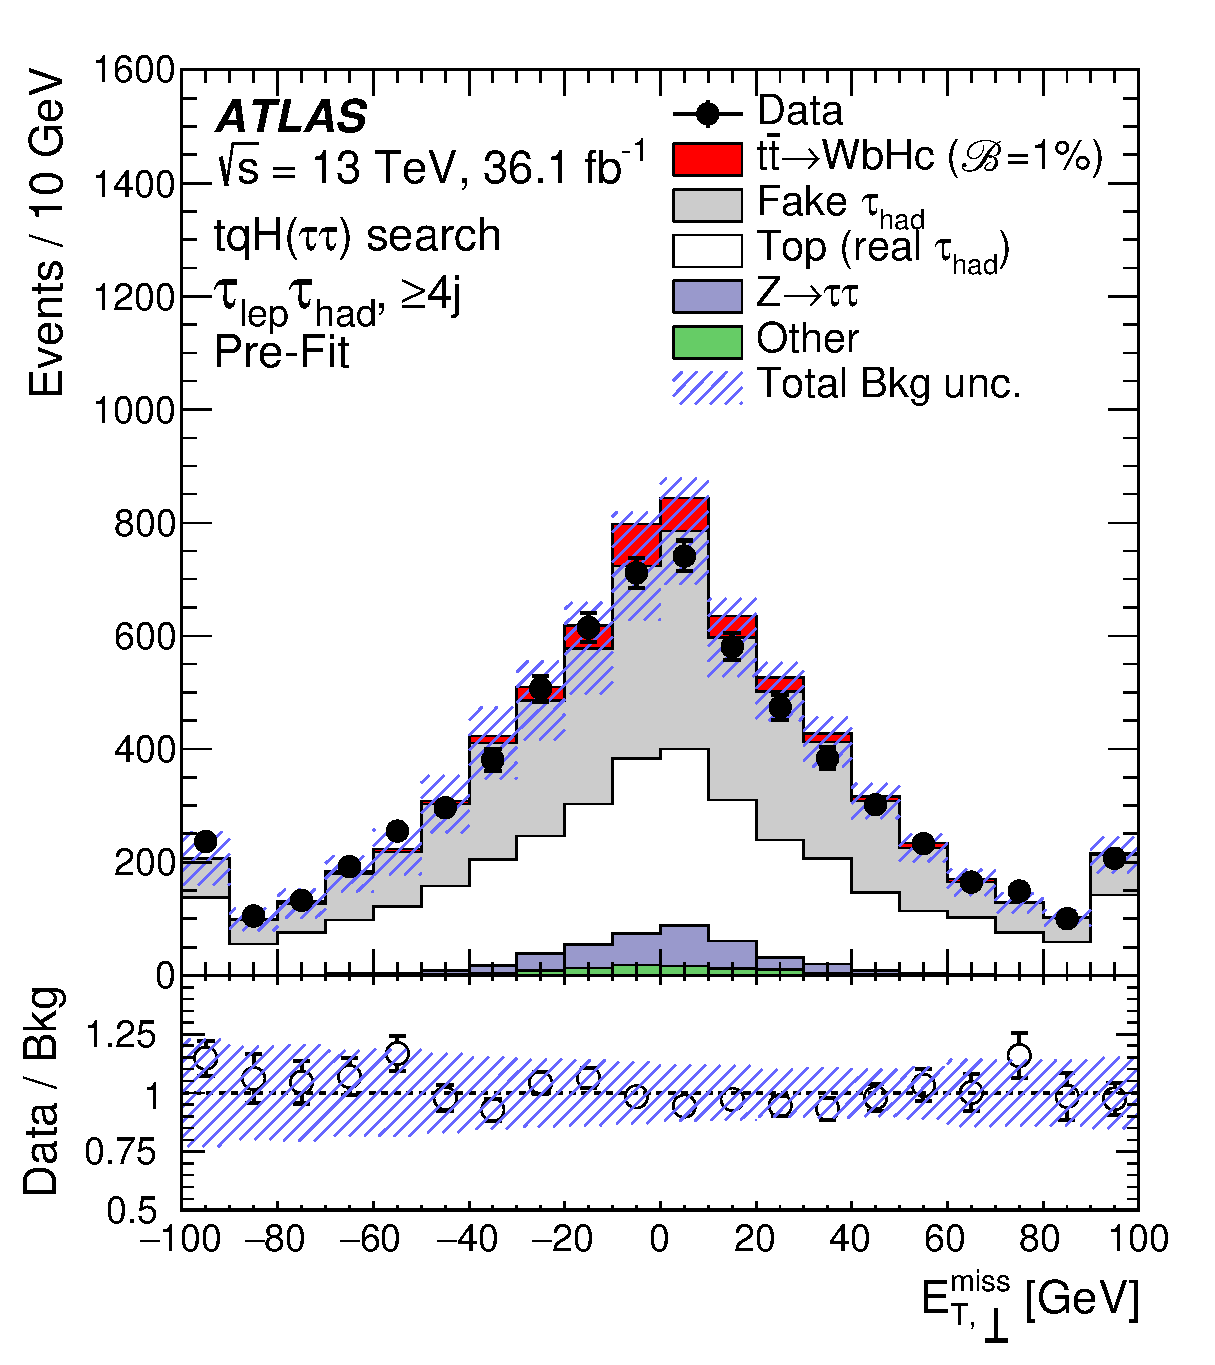
\includegraphics[width=0.40\textwidth]{figures/Htautau/control_plots/MET_perp_lephad_4j_FR.eps}} \\
\subfloat[]{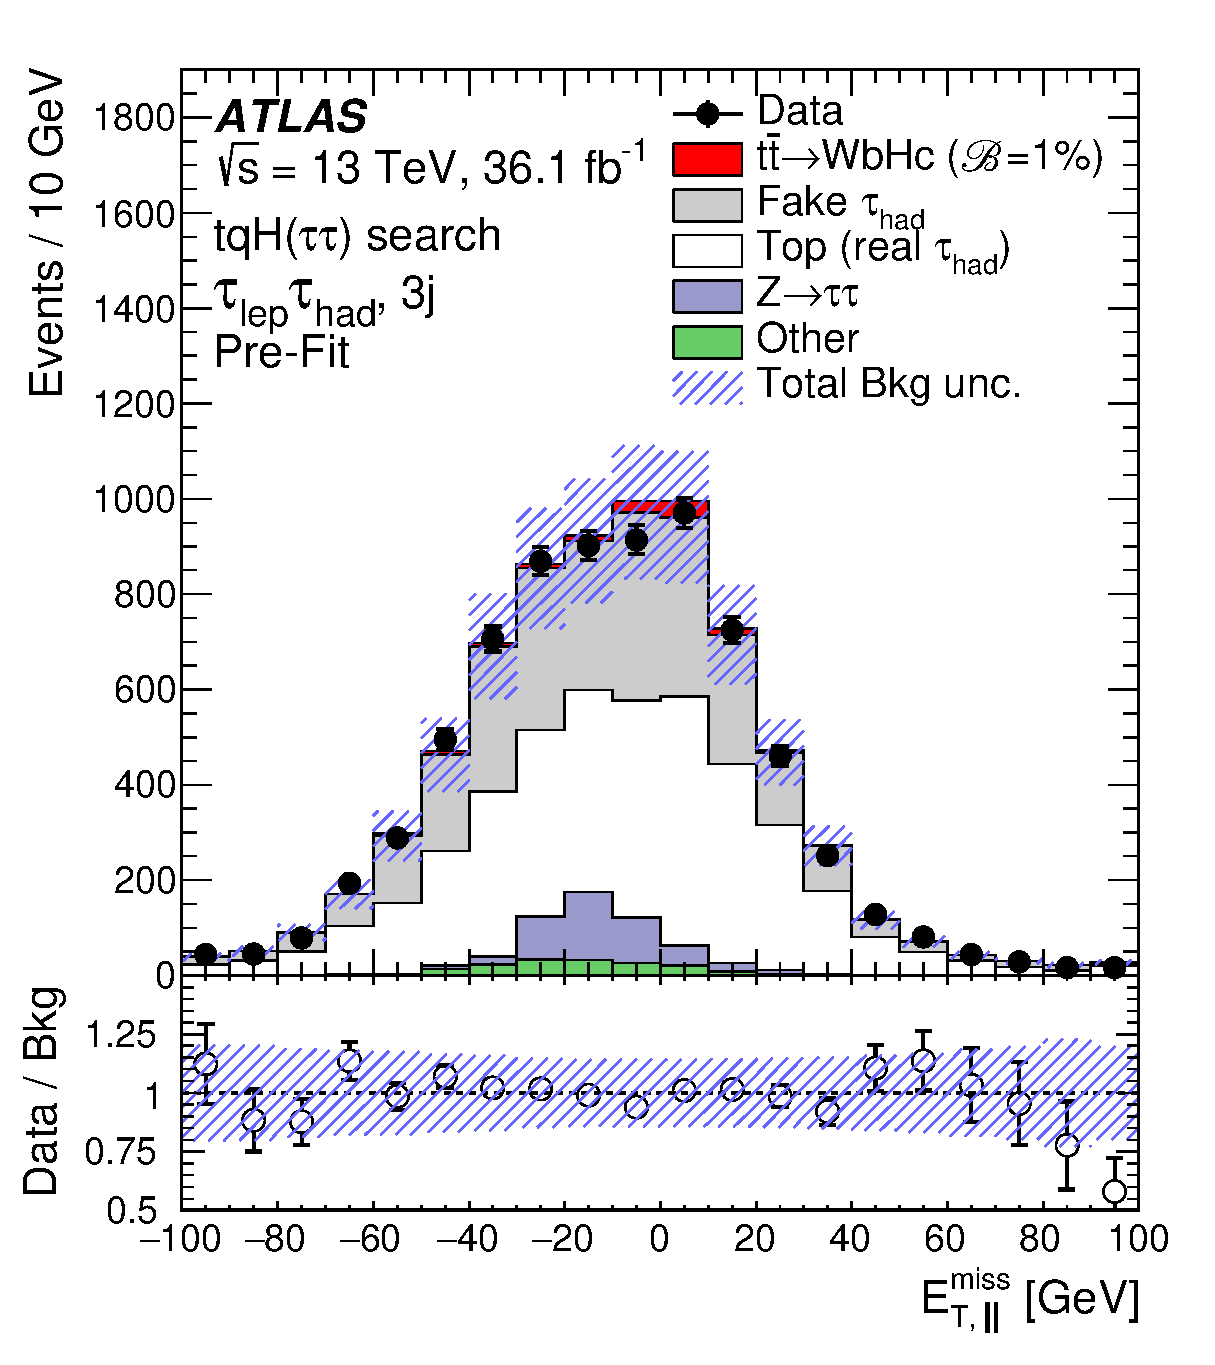
\includegraphics[width=0.40\textwidth]{figures/Htautau/control_plots/MET_proj_lephad_3j_FR.eps}}
\subfloat[]{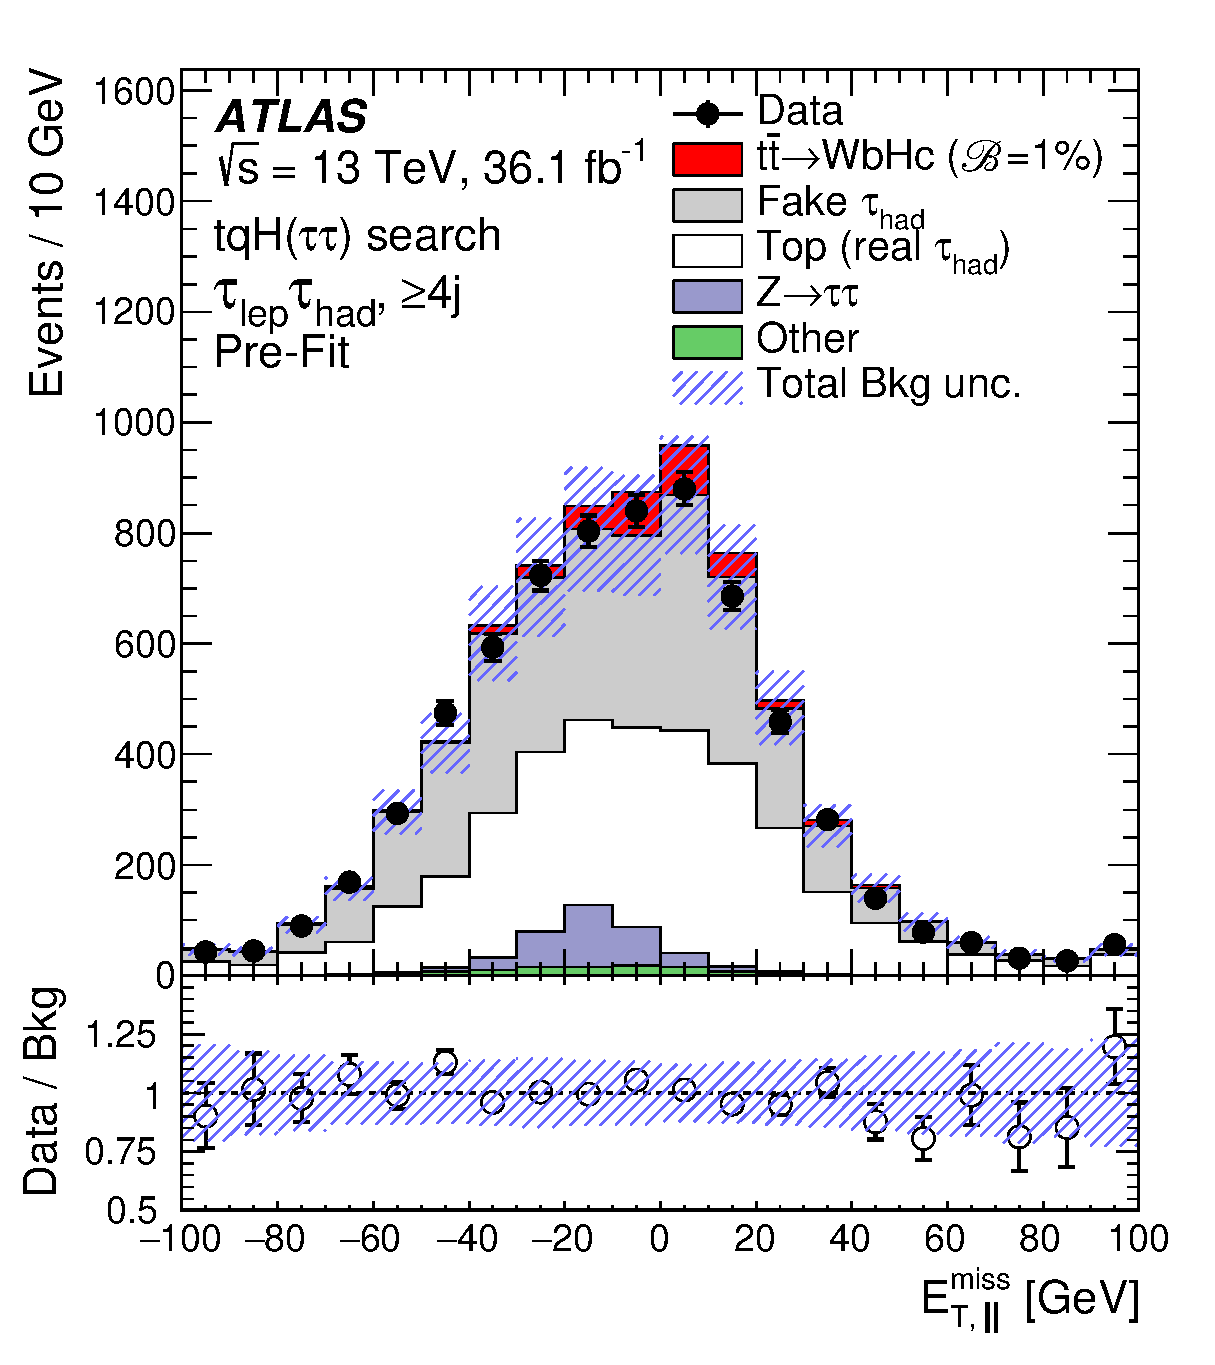
\includegraphics[width=0.40\textwidth]{figures/Htautau/control_plots/MET_proj_lephad_4j_FR.eps}} \\
\caption{$\Htautau$ search: Comparison between the data and background prediction for the distribution of some of the most
discriminating BDT input variables in the $\lephad$ channel before the fit to data (``Pre-Fit''). The distributions are shown for
$E_{\text{T},\perp}^{\text{miss}}$ in (a) the ($\lephad$, 3j) region and (b) the ($\lephad$, $\geq$4j) region, and for
$E_{\text{T},\parallel}^{\text{miss}}$ in (c) the ($\lephad$, 3j)  region and (d) the ($\lephad$, $\geq$4j) region.
The contributions with real $\had$ candidates from $\ttbar$,  $\ttbar V$, $\ttbar H$, and single top backgrounds are combined into
a single background source referred to as ``Top (real $\had$)", whereas the small contributions from 
$Z\to \ell^+\ell^-$ ($\ell = e, \mu$) and diboson backgrounds are combined into ``Other''. 
The expected $\Hc$ signal (solid red) corresponding to $\BR(t\to Hc)=1\%$ is also shown,
added to the background prediction.
%The first and the last bins in all figures contain the underflow and overflow respectively.
The bottom panel displays the ratio of data to the SM background (``Bkg'') prediction.
The hashed area represents the total uncertainty of the background, excluding the normalisation uncertainty of the fake $\had$ background, 
which is determined via a likelihood fit to data.}
\label{fig:BDT_inputs_lephad_4}
\end{center}
\end{figure*}
%%%%%%%%%%%%%%%%%%%%%%%%%%%%%%%%%%%%%%%



%%%%%%%%%%%%%%%%%%%%%%%%%%%%%%%%%%%%%%%
\begin{figure*}[t]
\begin{center}
\subfloat[]{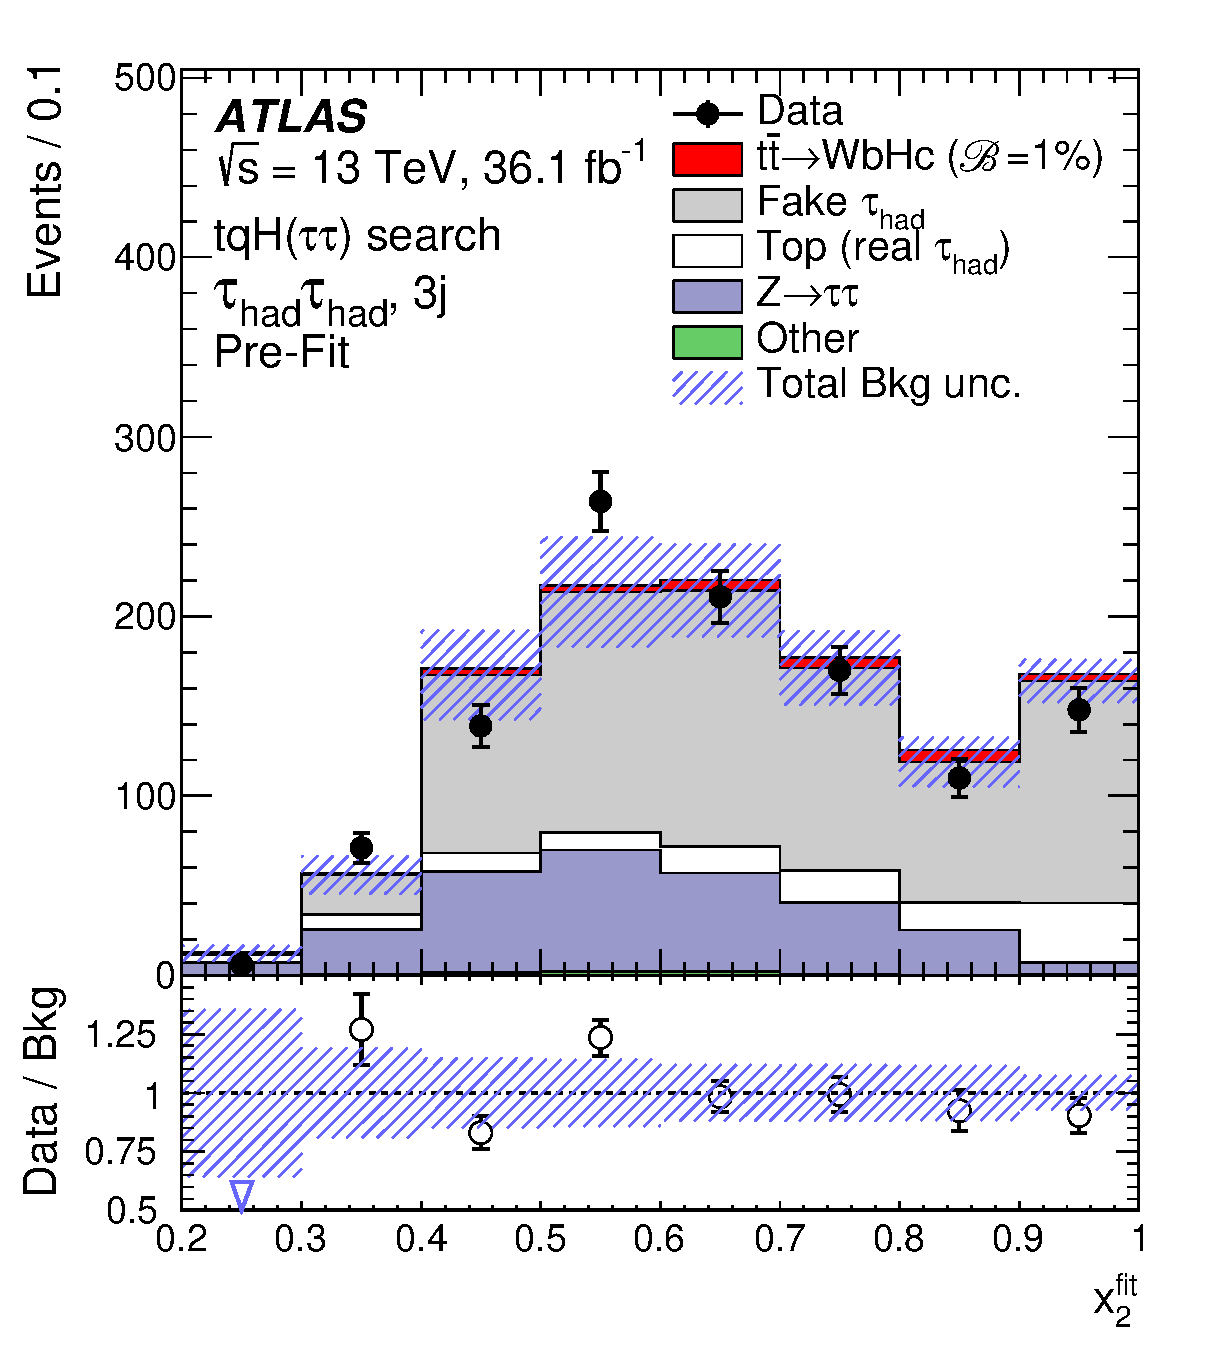
\includegraphics[width=0.40\textwidth]{figures/Htautau/control_plots/x2_fit_hadhad_3j_FR.eps}}
\subfloat[]{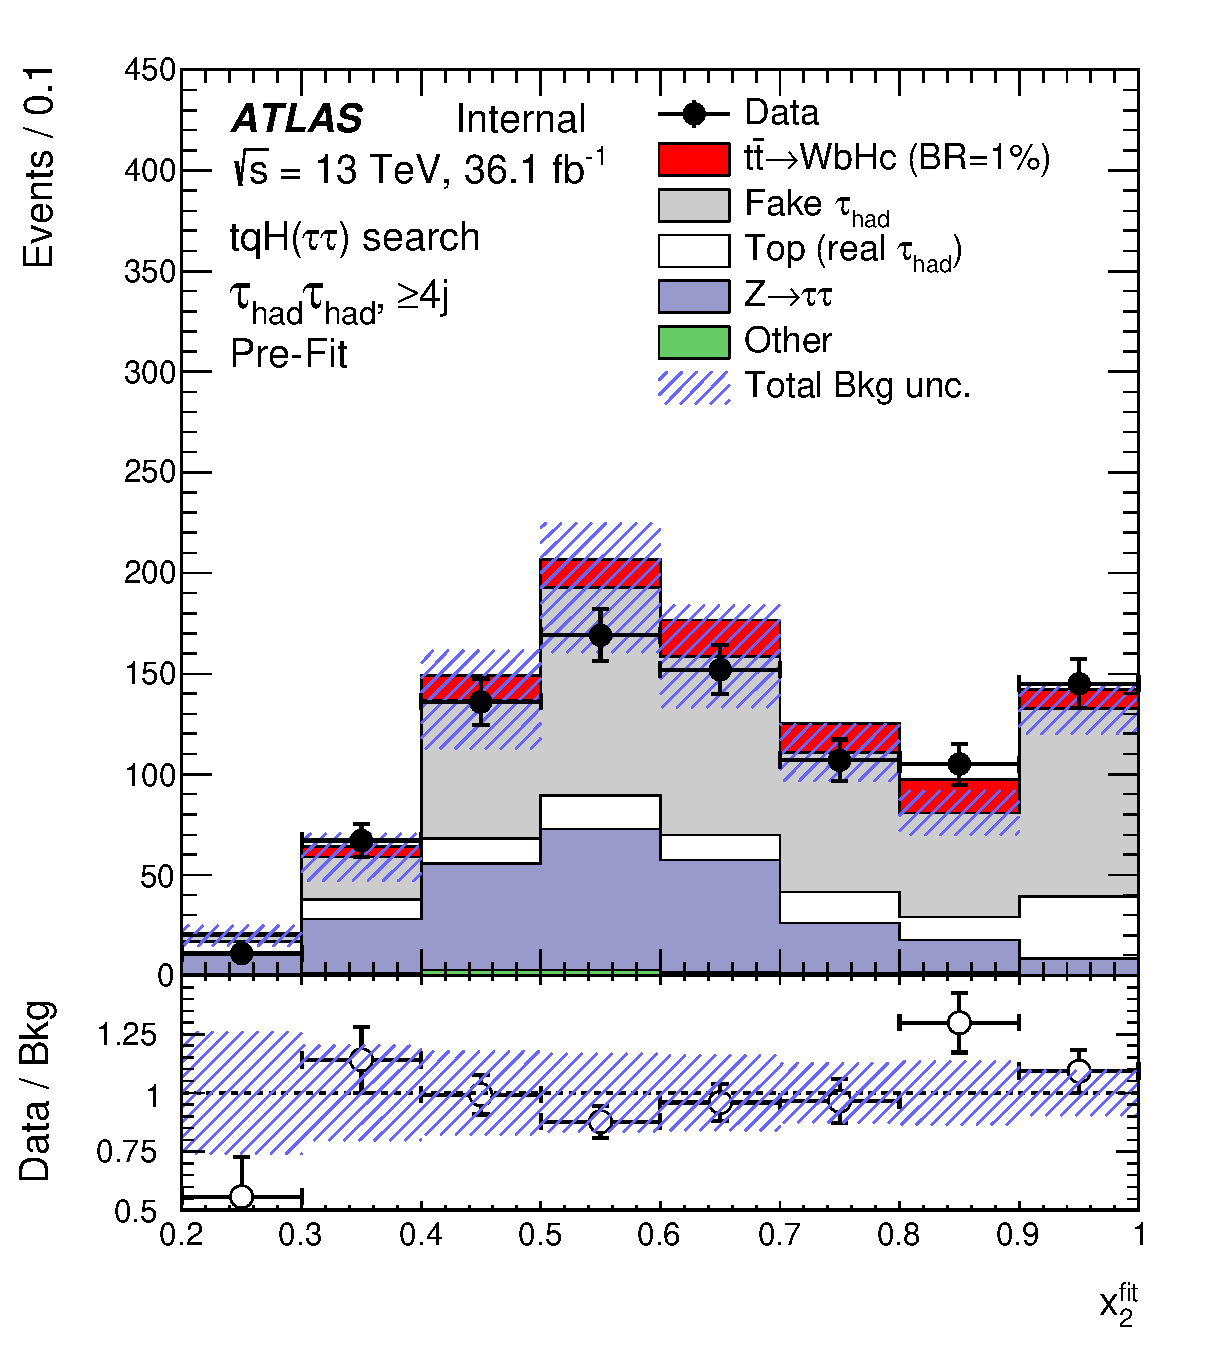
\includegraphics[width=0.40\textwidth]{figures/Htautau/control_plots/x2_fit_hadhad_4j_FR.eps}} \\
\subfloat[]{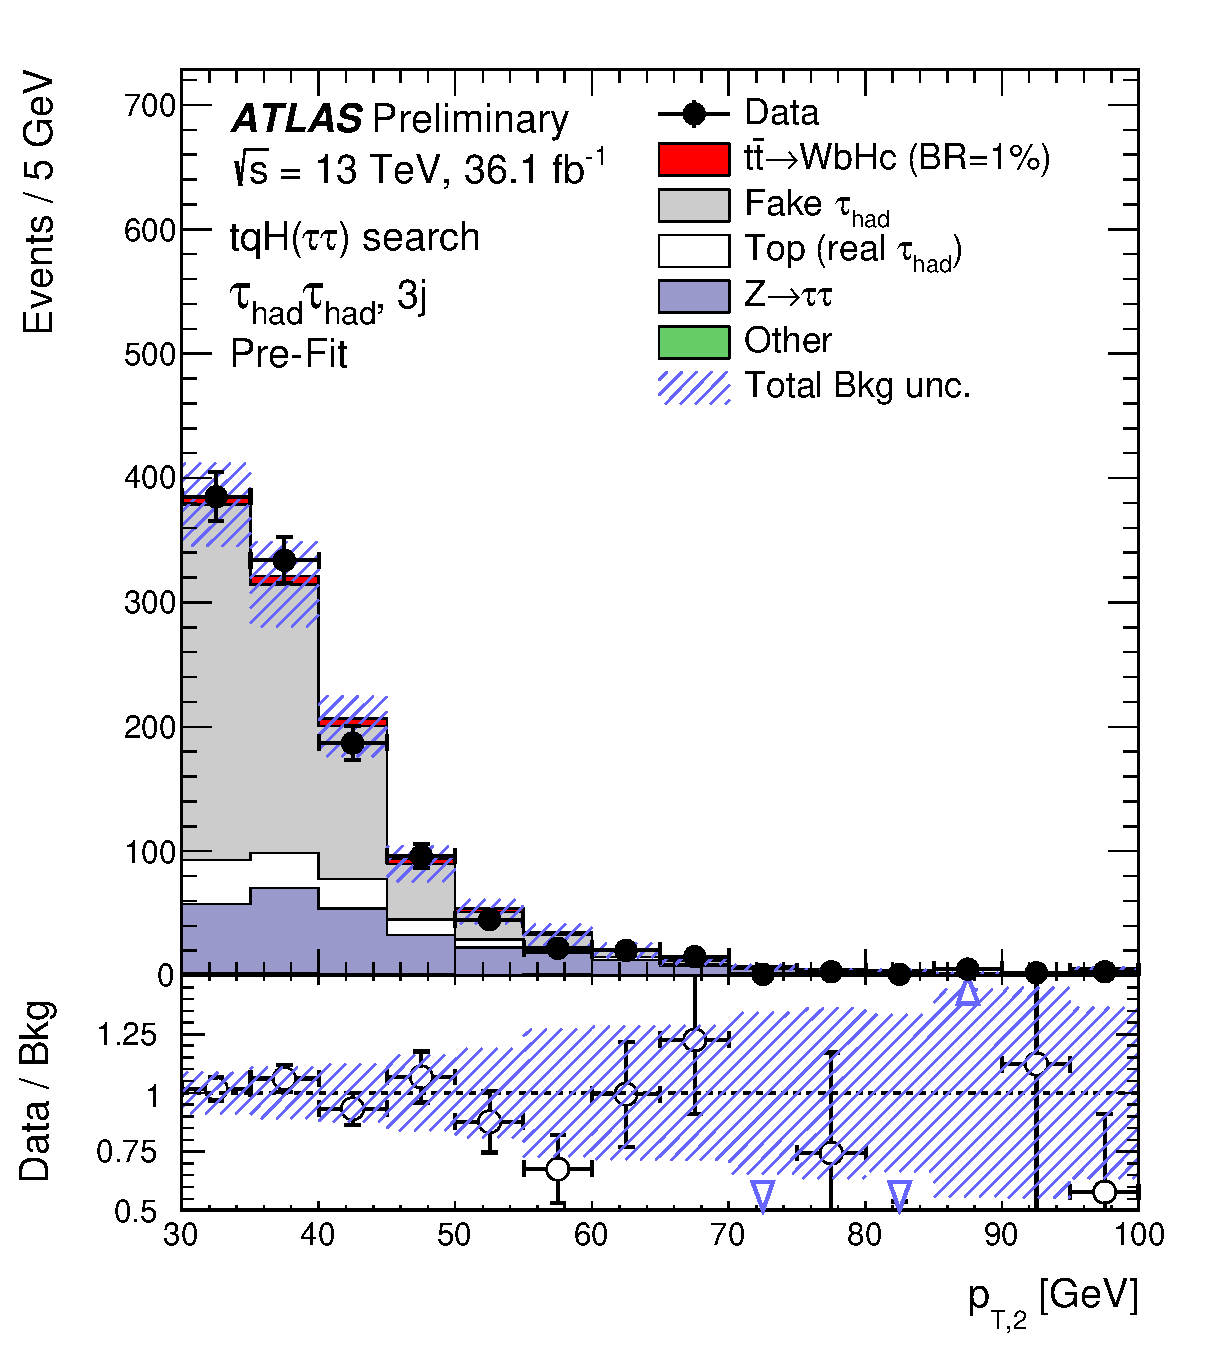
\includegraphics[width=0.40\textwidth]{figures/Htautau/control_plots/ptL2_hadhad_3j_FR.eps}}
\subfloat[]{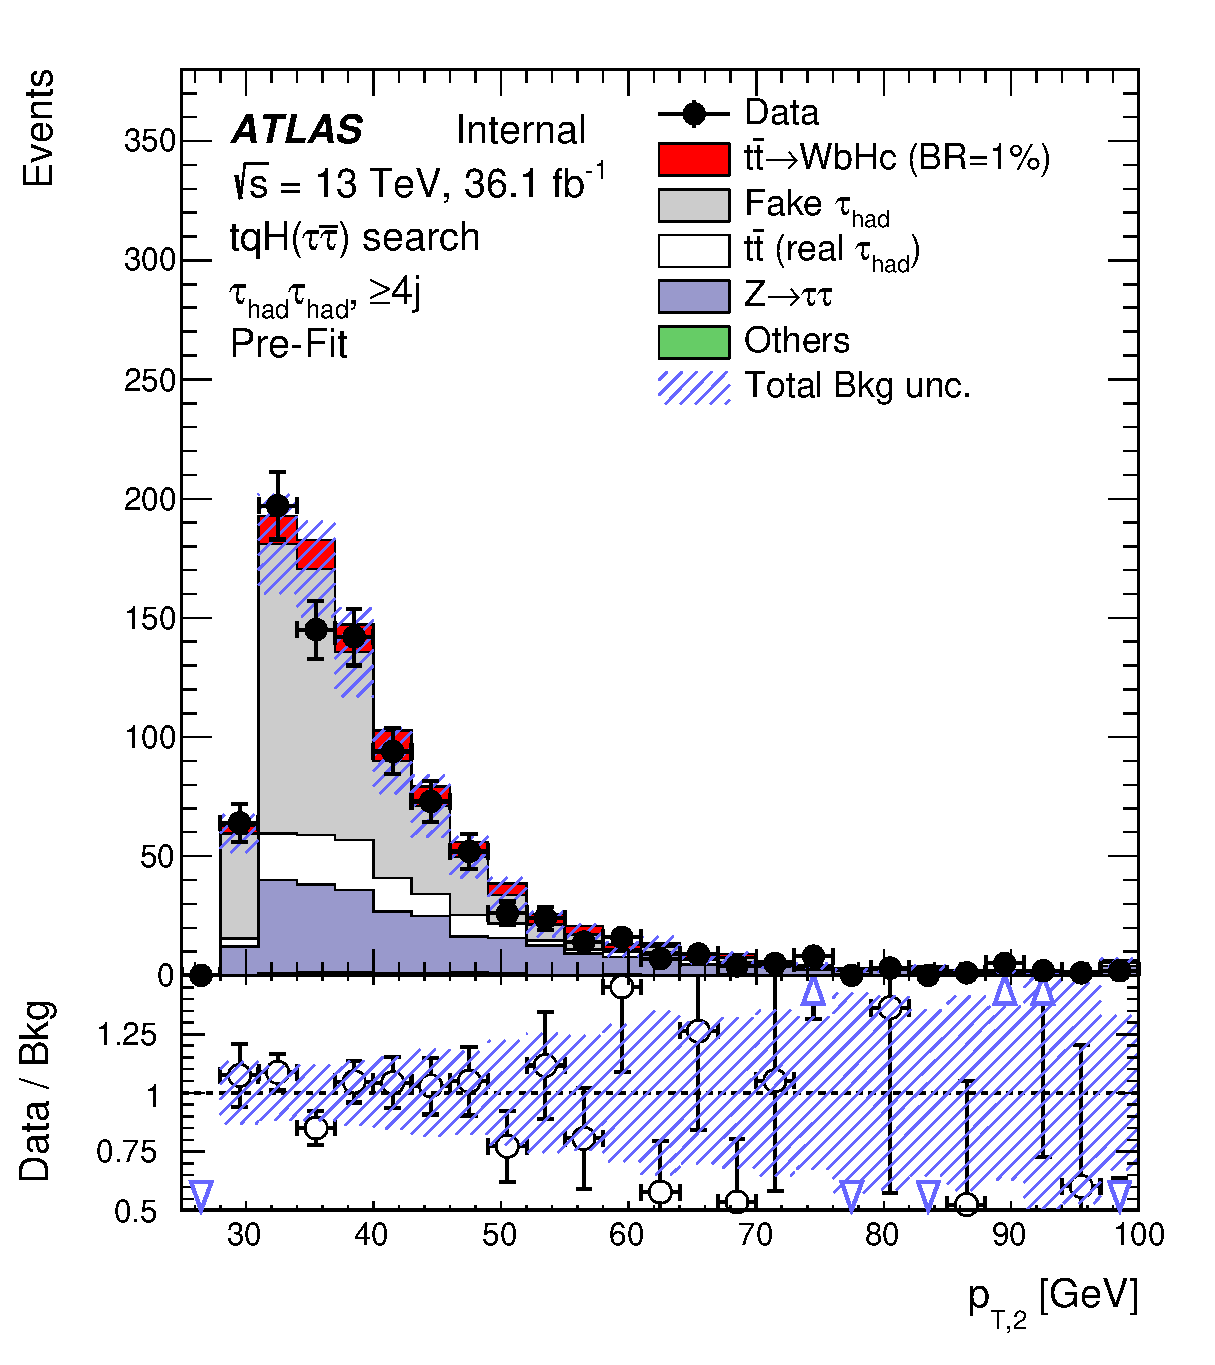
\includegraphics[width=0.40\textwidth]{figures/Htautau/control_plots/ptL2_hadhad_4j_FR.eps}} \\
\caption{$\Htautau$ search: Comparison between the data and background prediction for the distribution of two of the most 
discriminating BDT input variables in the $\hadhad$ channel before the fit to data (``Pre-Fit''). The distributions are shown for
$x_{2}^{\text{fit}}$ in (a) the ($\hadhad$, 3j) region and (b) the ($\hadhad$, $\geq$4j) region, and for
$p_{\text{T},2}$ in (c) the ($\hadhad$, 3j)  region and (d) the ($\hadhad$, $\geq$4j) region.
The contributions with real $\had$ candidates from $\ttbar$,  $\ttbar V$, $\ttbar H$, and single top backgrounds are combined into
a single background source referred to as ``Top (real $\had$)", whereas the small contributions from 
$Z\to \ell^+\ell^-$ ($\ell = e, \mu$) and diboson backgrounds are combined into ``Other''. 
The expected $\Hc$ signal (solid red) corresponding to $\BR(t\to Hc)=1\%$ is also shown,
added to the background prediction.
The first and the last bins in the figures in (c) and (d) contain the underflow and overflow respectively.
The bottom panel displays the ratio of data to the SM background (``Bkg'') prediction.
The hashed area represents the total uncertainty of the background, excluding the normalisation uncertainty of the fake $\had$ background, 
which is determined via a likelihood fit to data.} 
\label{fig:BDT_inputs_hadhad_2}
\end{center}
\end{figure*}
%%%%%%%%%%%%%%%%%%%%%%%%%%%%%%%%%%%%%%%

%%%%%%%%%%%%%%%%%%%%%%%%%%%%%%%%%%%%%%%
\begin{figure*}[t]
\begin{center}
\subfloat[]{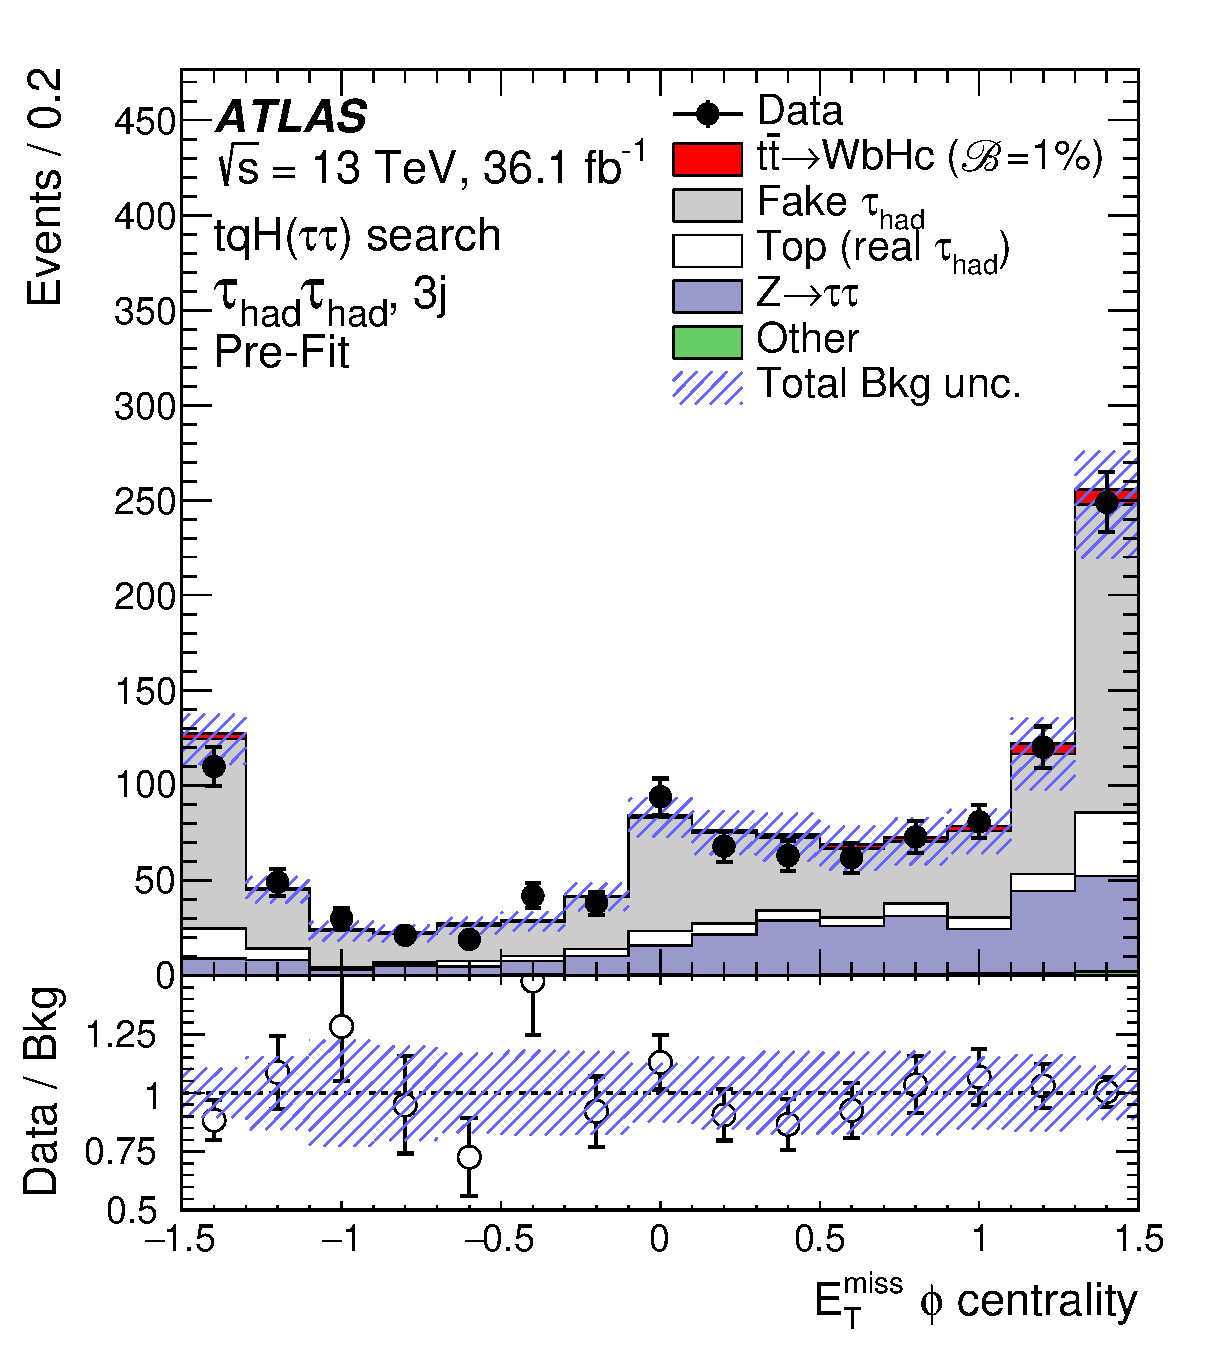
\includegraphics[width=0.40\textwidth]{figures/Htautau/control_plots/met_centrality_hadhad_3j_FR.eps}}
\subfloat[]{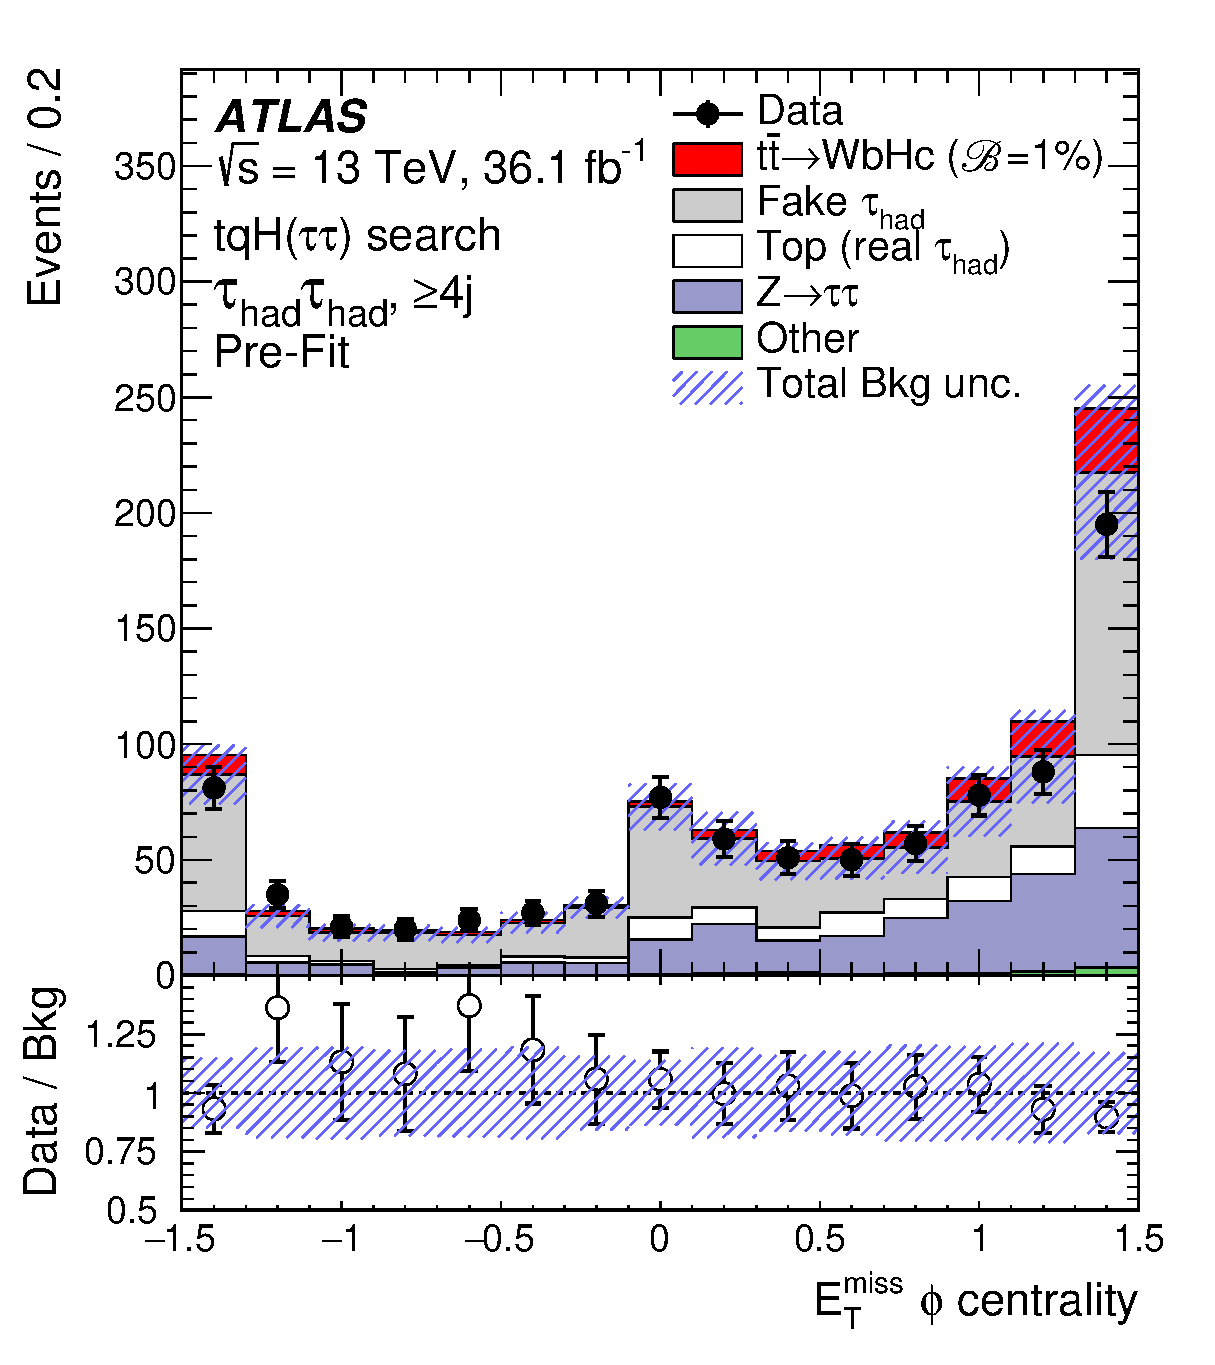
\includegraphics[width=0.40\textwidth]{figures/Htautau/control_plots/met_centrality_hadhad_4j_FR.eps}} \\
\subfloat[]{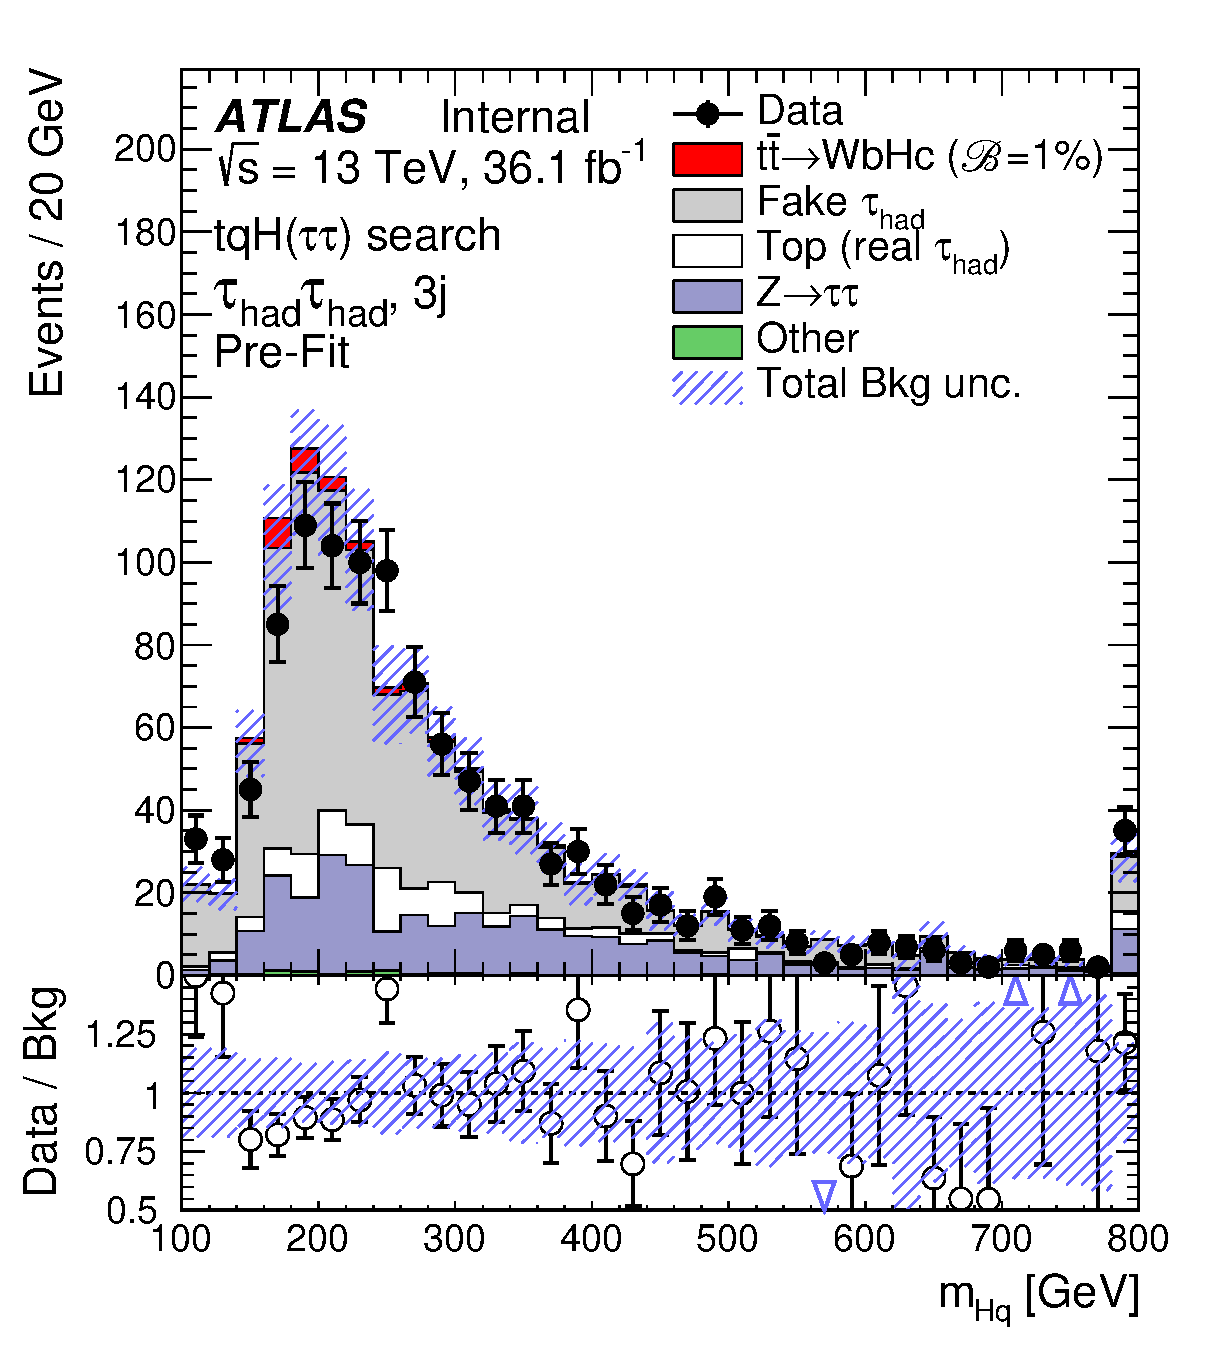
\includegraphics[width=0.40\textwidth]{figures/Htautau/control_plots/mtop_thc_hadhad_3j_FR.eps}}
\subfloat[]{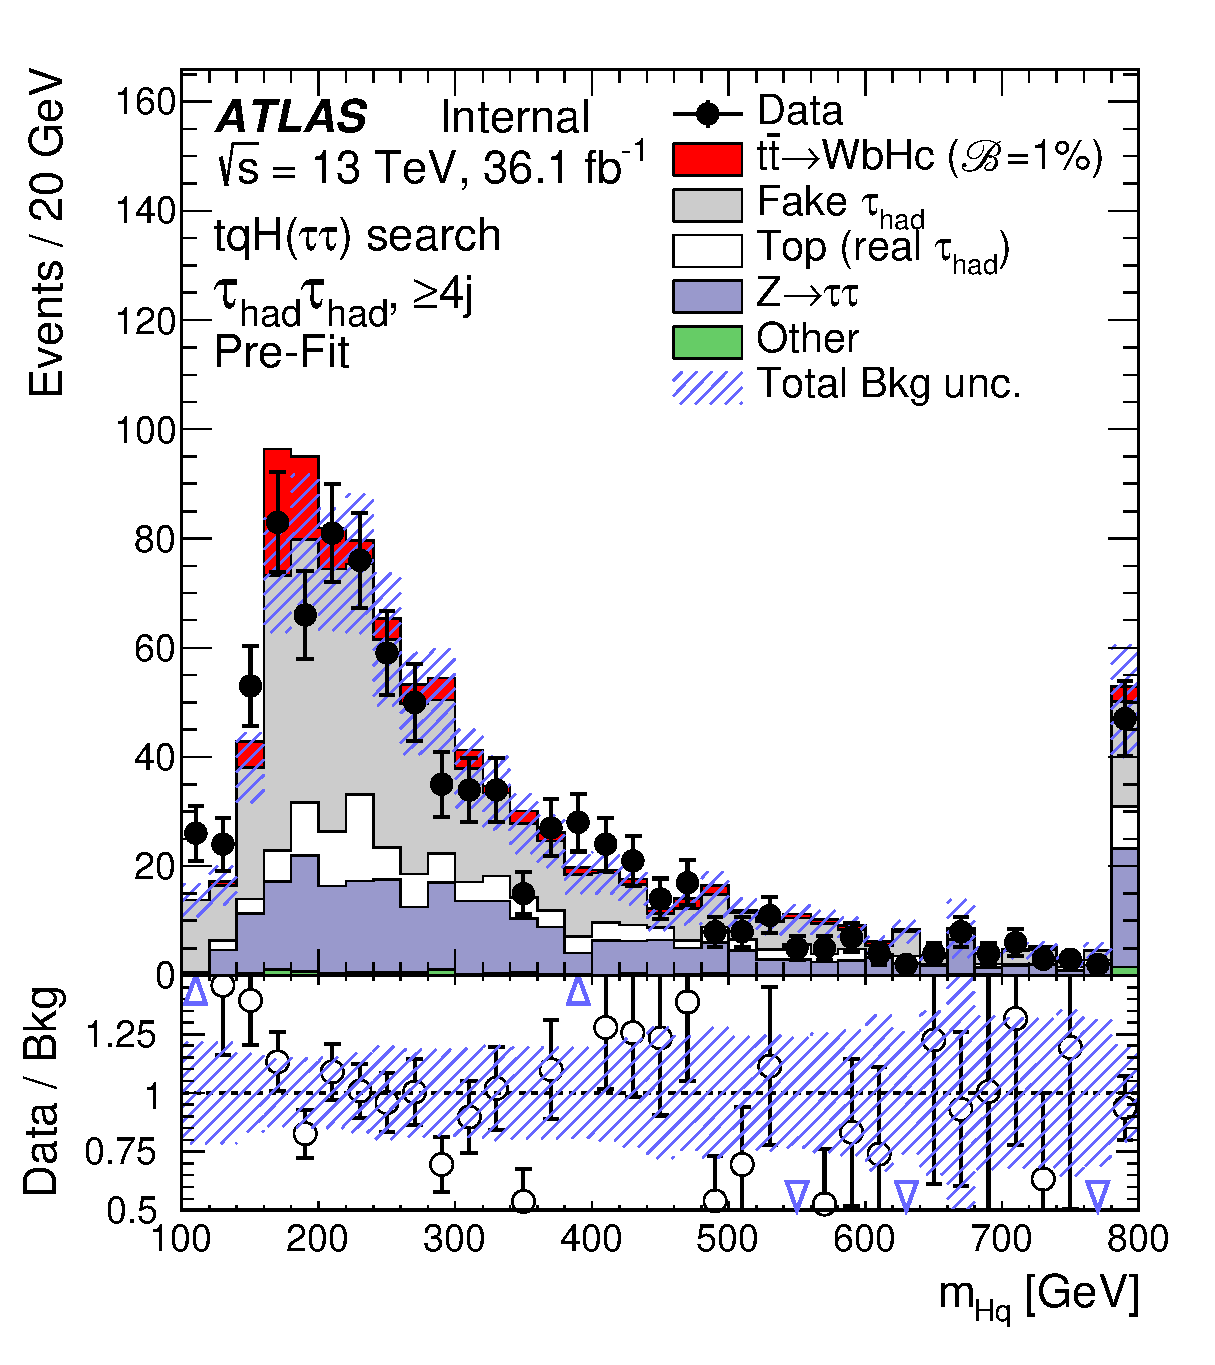
\includegraphics[width=0.40\textwidth]{figures/Htautau/control_plots/mtop_thc_hadhad_4j_FR.eps}} \\
\caption{$\Htautau$ search: Comparison between the data and background prediction for the distribution of two of the most 
discriminating BDT input variables in the $\hadhad$ channel before the fit to data (``Pre-Fit''). The distributions are shown for
$\met$ $\phi$ centrality  in (a) the ($\hadhad$, 3j) region and (b) the ($\hadhad$, $\geq$4j) region, and for
$m_{Hq}$ in (c) the ($\hadhad$, 3j)  region and (d) the ($\hadhad$, $\geq$4j) region.
The contributions with real $\had$ candidates from $\ttbar$,  $\ttbar V$, $\ttbar H$, and single top backgrounds are combined into
a single background source referred to as ``Top (real $\had$)", whereas the small contributions from 
$Z\to \ell^+\ell^-$ ($\ell = e, \mu$) and diboson backgrounds are combined into ``Other''. 
The expected $\Hc$ signal (solid red) corresponding to $\BR(t\to Hc)=1\%$ is also shown,
added to the background prediction.
The first and the last bins in the figures in (c) and (d) contain the underflow and overflow respectively.
The bottom panel displays the ratio of data to the SM background (``Bkg'') prediction.
The hashed area represents the total uncertainty of the background, excluding the normalisation uncertainty of the fake $\had$ background, 
which is determined via a likelihood fit to data.} 
\label{fig:BDT_inputs_hadhad_3}
\end{center}
\end{figure*}
%%%%%%%%%%%%%%%%%%%%%%%%%%%%%%%%%%%%%%%


%%%%%%%%%%%%%%%%%%%%%%%%%%%%%%%%%%%%%%%
\begin{figure*}[t]
\begin{center}
\subfloat[]{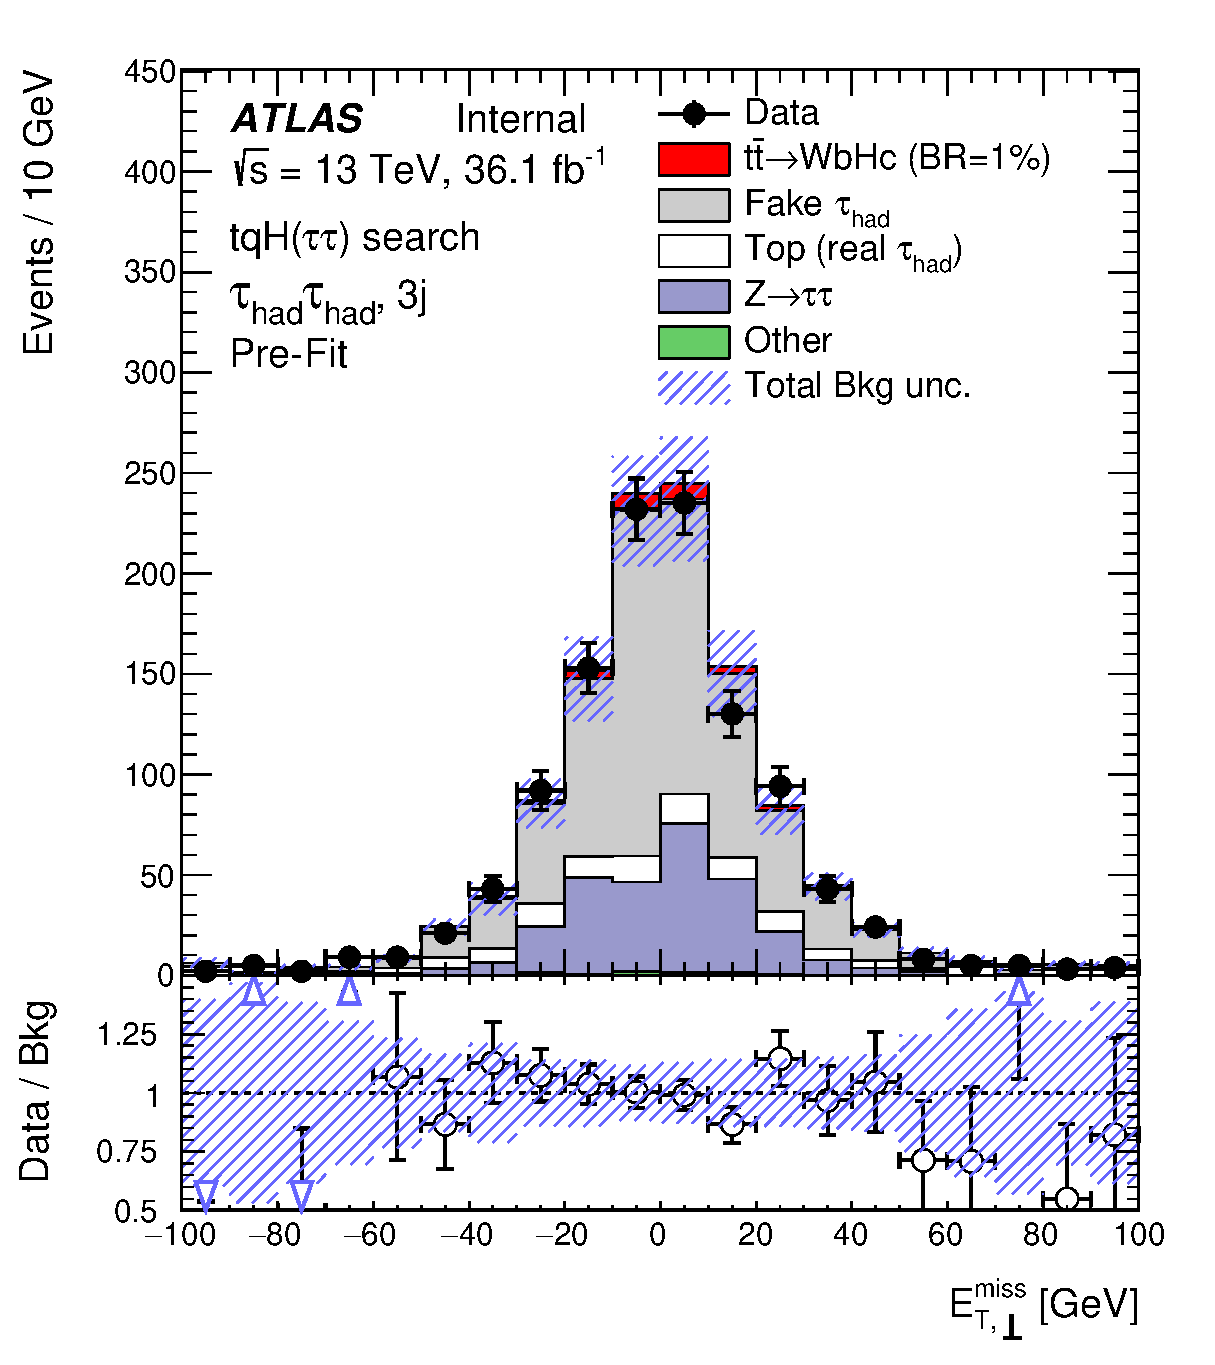
\includegraphics[width=0.40\textwidth]{figures/Htautau/control_plots/MET_perp_hadhad_3j_FR.eps}}
\subfloat[]{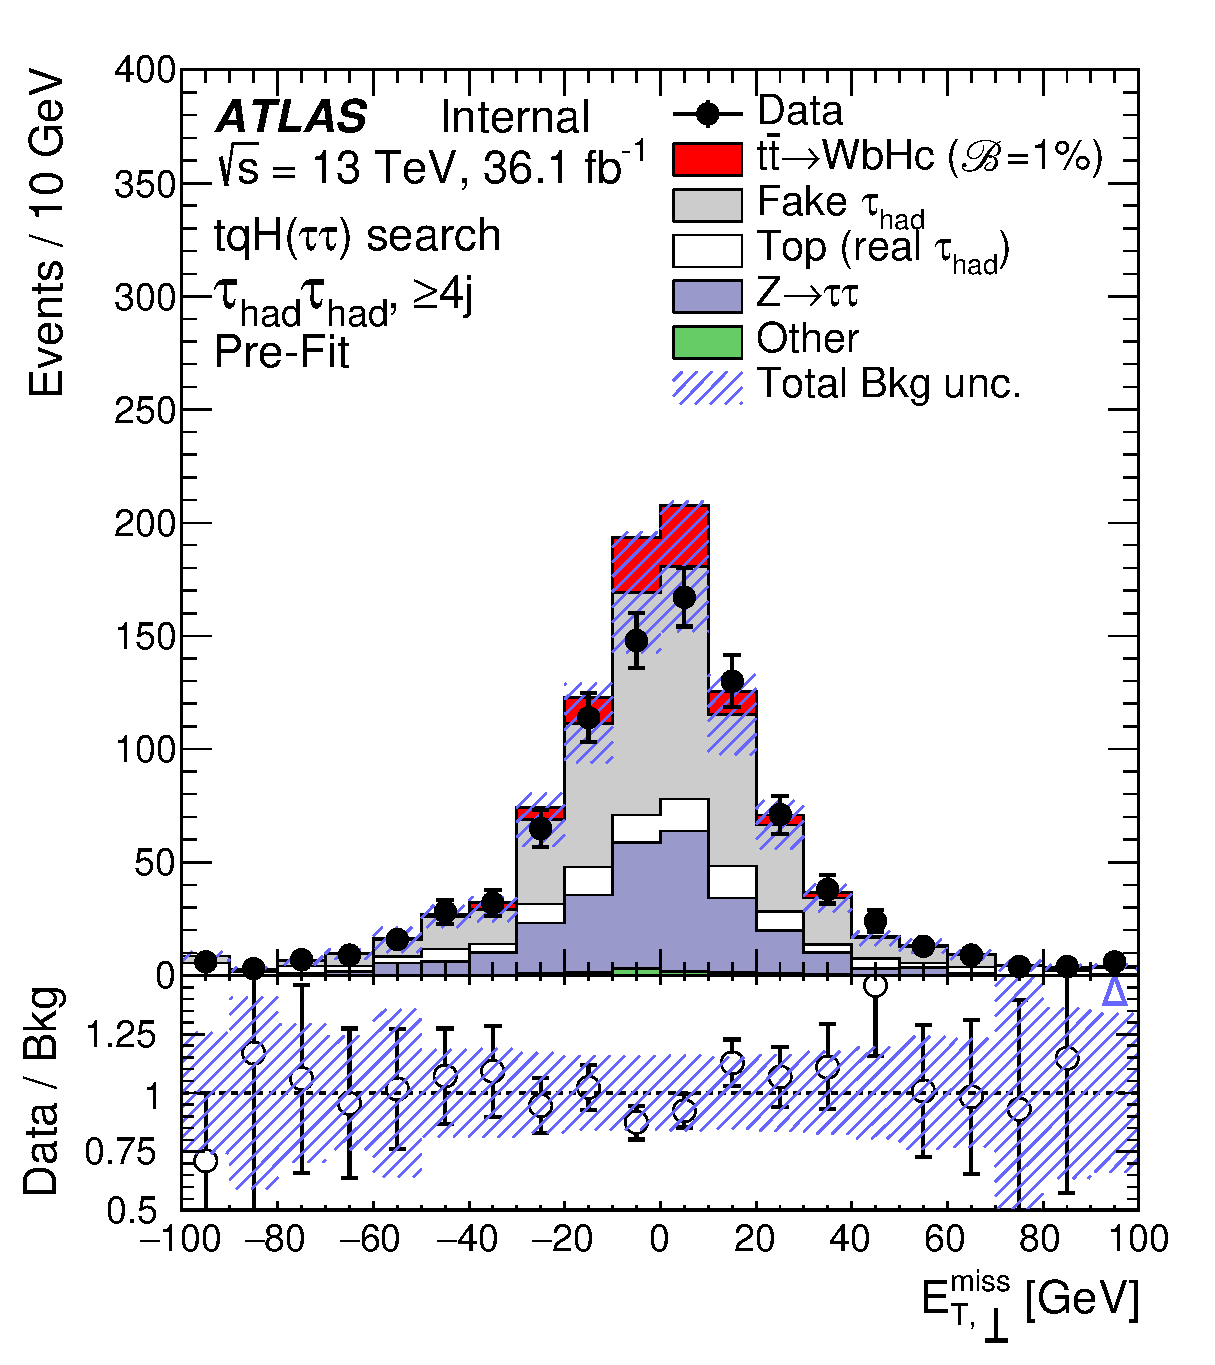
\includegraphics[width=0.40\textwidth]{figures/Htautau/control_plots/MET_perp_hadhad_4j_FR.eps}} \\
\subfloat[]{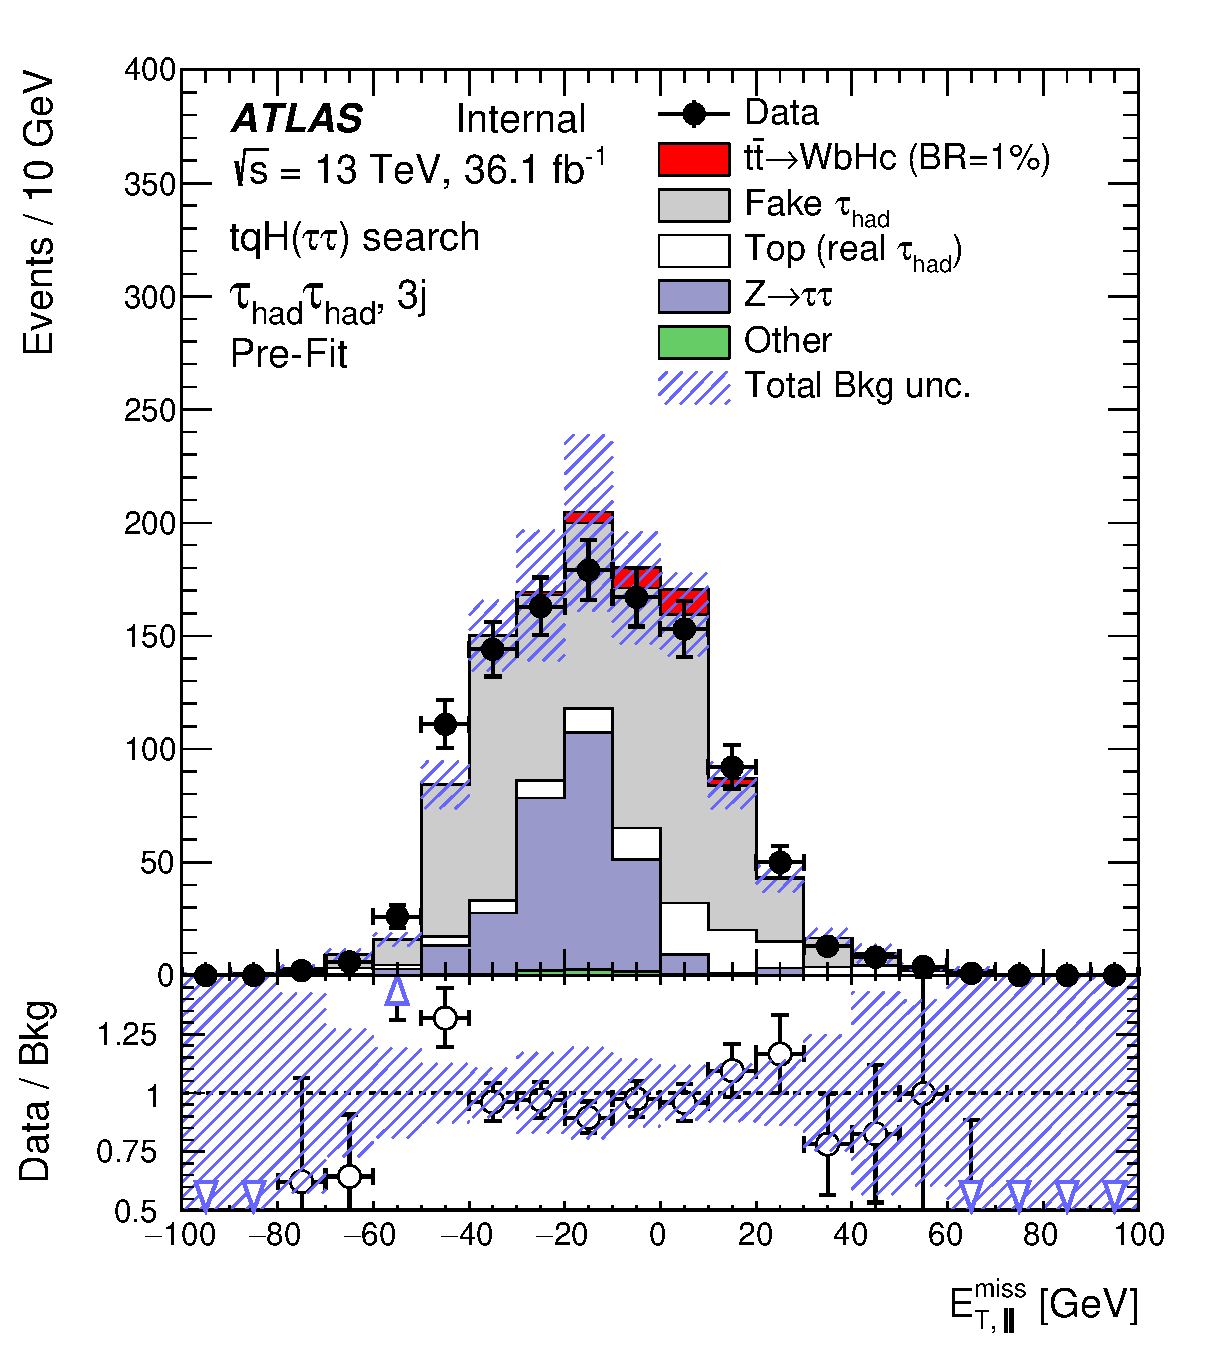
\includegraphics[width=0.40\textwidth]{figures/Htautau/control_plots/MET_proj_hadhad_3j_FR.eps}}
\subfloat[]{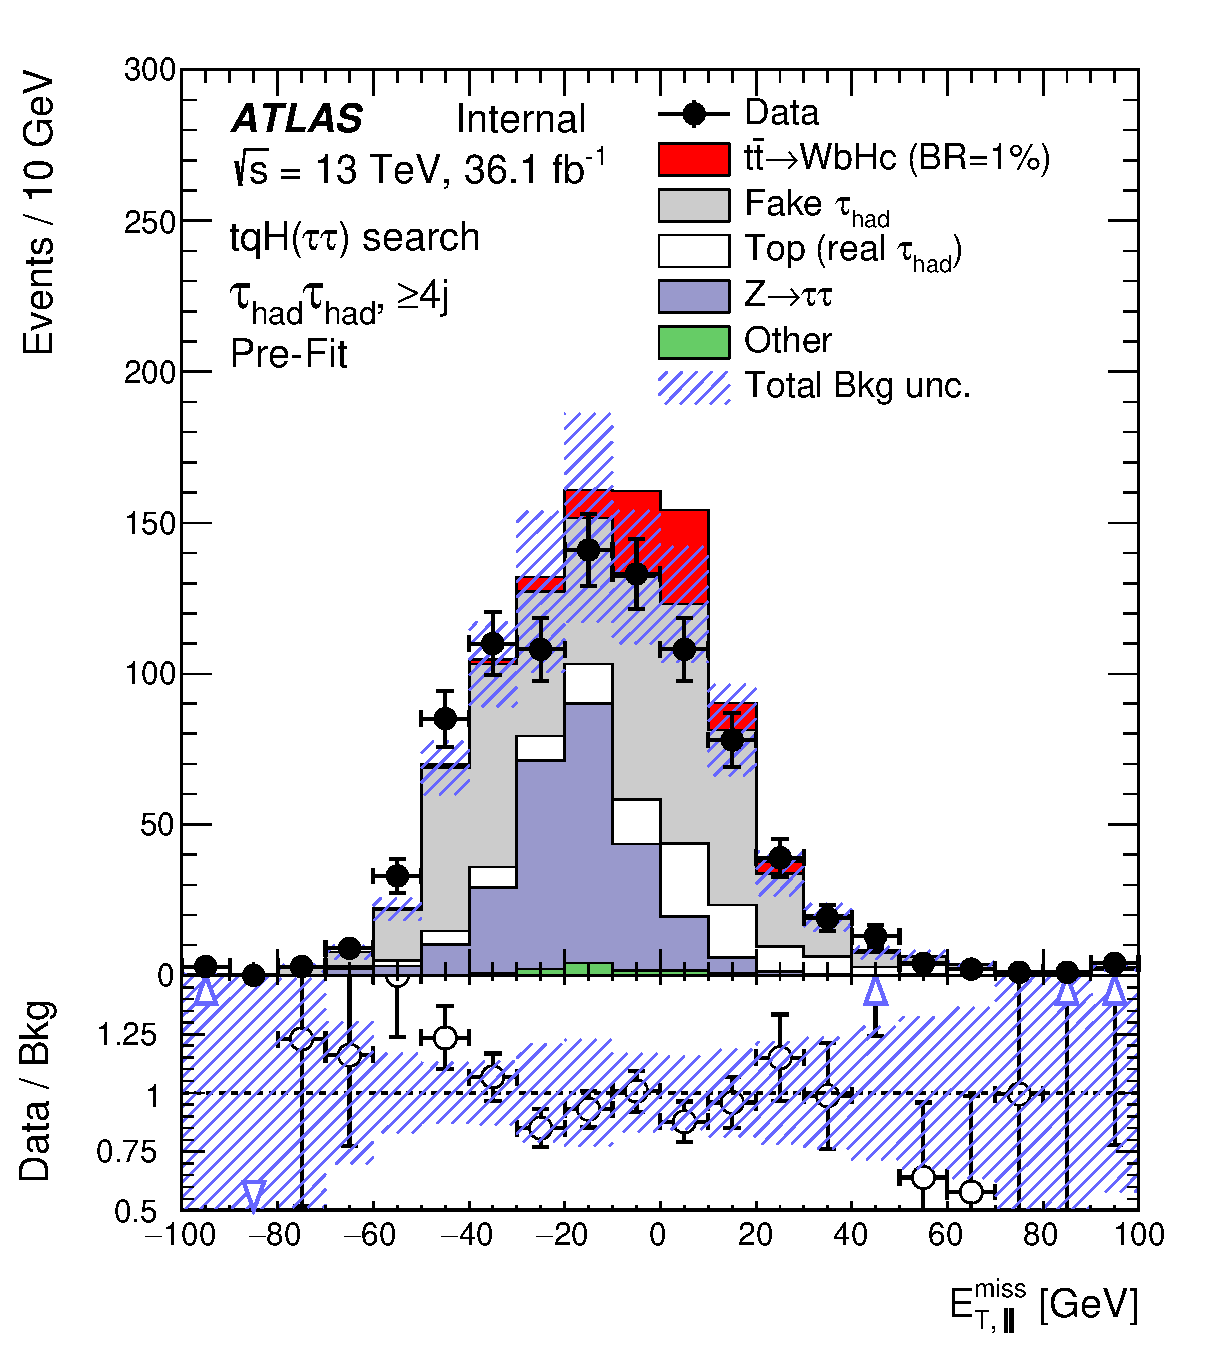
\includegraphics[width=0.40\textwidth]{figures/Htautau/control_plots/MET_proj_hadhad_4j_FR.eps}} \\
\caption{$\Htautau$ search: Comparison between the data and background prediction for the distribution of two of the most 
discriminating BDT input variables in the $\hadhad$ channel before the fit to data (``Pre-Fit''). The distributions are shown for
$E_{\text{T},\perp}^{\text{miss}}$ in (a) the ($\hadhad$, 3j) region and (b) the ($\hadhad$, $\geq$4j) region, and for
$E_{\text{T},\parallel}^{\text{miss}}$ in (c) the ($\hadhad$, 3j)  region and (d) the ($\hadhad$, $\geq$4j) region.
The contributions with real $\had$ candidates from $\ttbar$,  $\ttbar V$, $\ttbar H$, and single top backgrounds are combined into
a single background source referred to as ``Top (real $\had$)", whereas the small contributions from 
$Z\to \ell^+\ell^-$ ($\ell = e, \mu$) and diboson backgrounds are combined into ``Other''. 
The expected $\Hc$ signal (solid red) corresponding to $\BR(t\to Hc)=1\%$ is also shown,
added to the background prediction.
The first and the last bins in the figures in (c) and (d) contain the underflow and overflow respectively.
The bottom panel displays the ratio of data to the SM background (``Bkg'') prediction.
The hashed area represents the total uncertainty of the background, excluding the normalisation uncertainty of the fake $\had$ background, 
which is determined via a likelihood fit to data.} 
\label{fig:BDT_inputs_hadhad_4}
\end{center}
\end{figure*}
%%%%%%%%%%%%%%%%%%%%%%%%%%%%%%%%%%%%%%%



%%%%%%%%%%%%%%%%%%%%%%%%%%%%%%%%%%%%%%%
\begin{figure*}[t]
\begin{center}
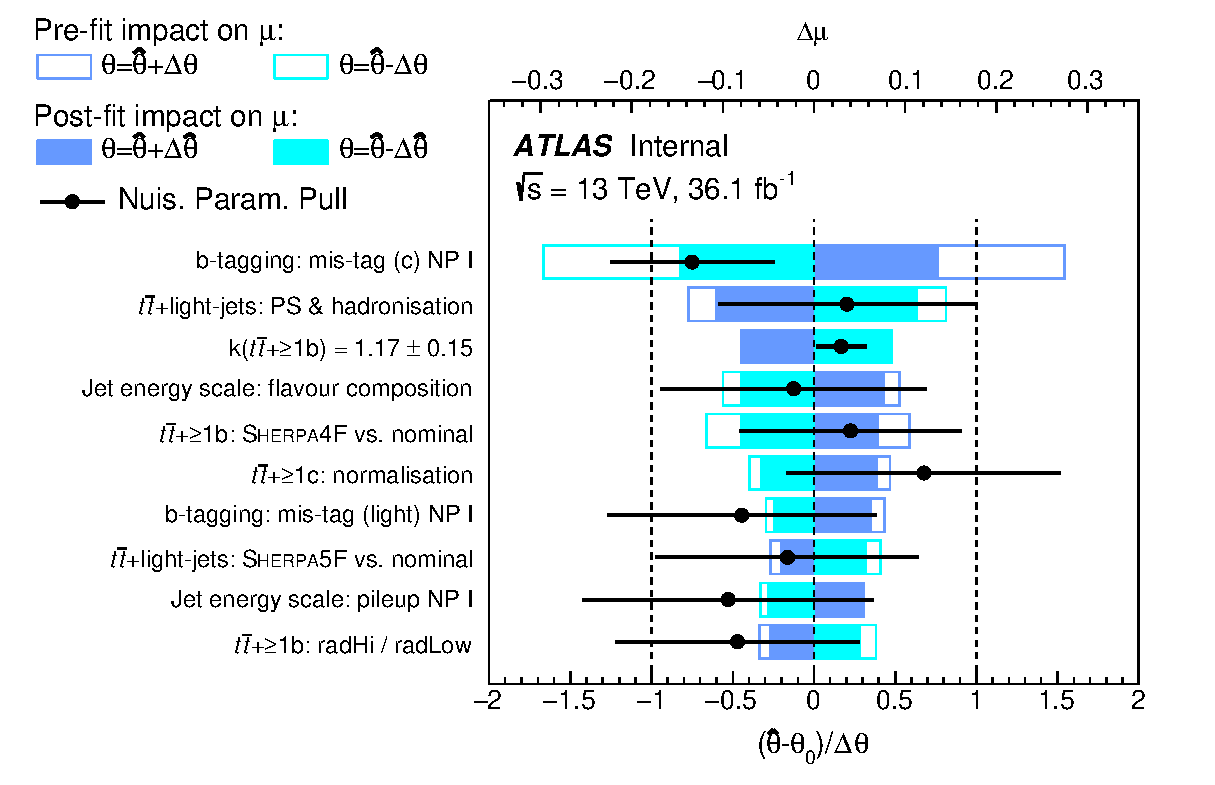
\includegraphics[width=0.90\textwidth]{figures/Combo/ranking/Ranking_bb.eps} \\
\caption{$\Hbb$ search: Ranking of the nuisance parameters included in the fit according to their impact on the measured signal strength $\mu$, in
the case of the $\Hc$ search.
Only the 10 most highly ranked parameters are shown. Nuisance parameters corresponding to MC statistical uncertainties are not included here. 
The empty blue rectangles correspond to the pre-fit impact on $\mu$ and the filled blue ones to the post-fit impact on $\mu$, 
both referring to the upper scale. The impact of each nuisance parameter, $\Delta\mu$, is computed by comparing the nominal best-fit value of $\mu$ 
with the result of the fit when fixing the considered nuisance parameter to its best-fit value, $\hat{\theta}$, shifted by its pre-fit (post-fit) uncertainties 
$\pm\Delta\theta$ ($\pm\Delta\hat{\theta}$). The black points show the pulls of the nuisance parameters relative to their nominal values, $\theta_{0}$. 
These pulls and their relative post-fit errors, $\Delta\hat{\theta}/\Delta\theta$, refer to the lower scale.
For experimental uncertainties that are decomposed into several independent sources, NP I corresponds to the first nuisance parameter, 
ordered by its impact on $\mu$.} 
\label{fig:ranking_bb}
\end{center}
\end{figure*}
%%%%%%%%%%%%%%%%%%%%%%%%%%%%%%%%%%%%%%%

%%%%%%%%%%%%%%%%%%%%%%%%%%%%%%%%%%%%%%%
\begin{figure*}[t]
\begin{center}
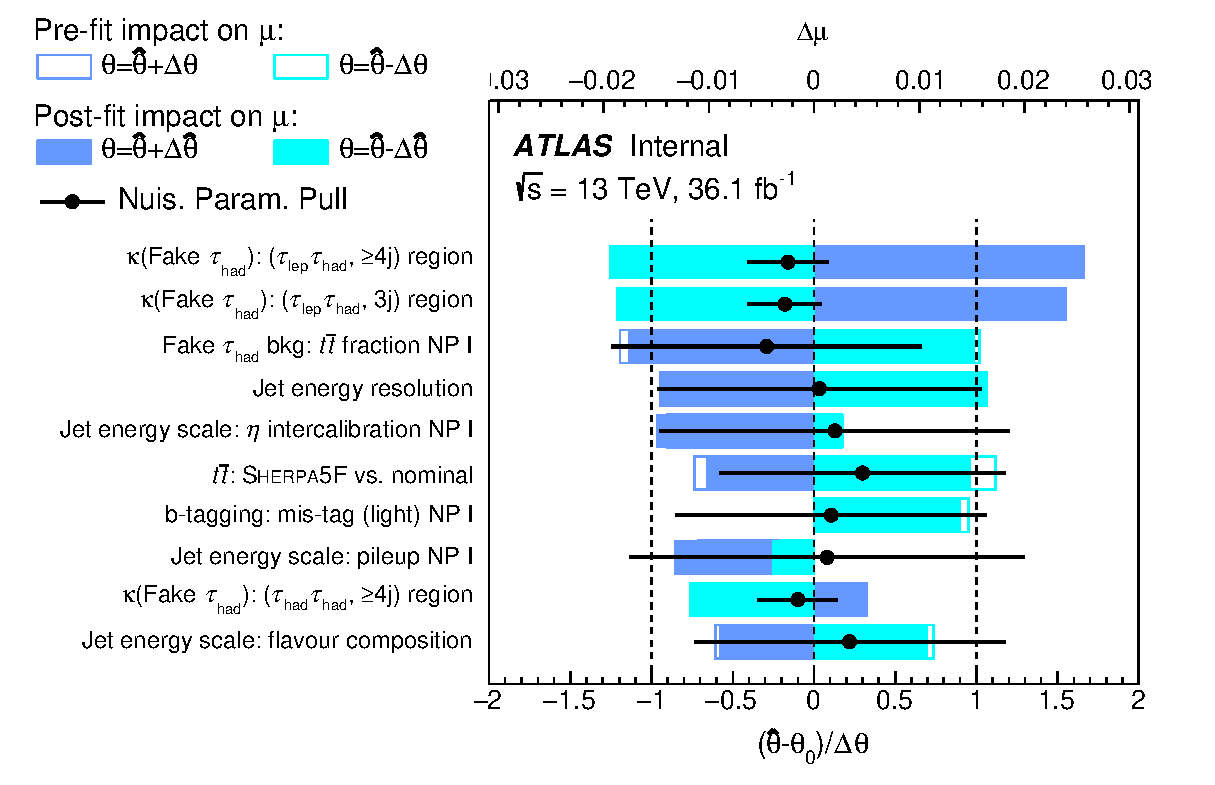
\includegraphics[width=0.90\textwidth]{figures/Combo/ranking/Ranking_tt.eps} \\
\caption{$\Htautau$ search: Ranking of the nuisance parameters included in the fit according to their impact on the measured signal strength $\mu$, in
the case of the $\Hc$ search.
Only the 10 most highly ranked parameters are shown. Nuisance parameters corresponding to MC statistical uncertainties are not included here. 
The empty blue rectangles correspond to the pre-fit impact on $\mu$ and the filled blue ones to the post-fit impact on $\mu$, 
both referring to the upper scale. The impact of each nuisance parameter, $\Delta\mu$, is computed by comparing the nominal best-fit value of $\mu$ 
with the result of the fit when fixing the considered nuisance parameter to its best-fit value, $\hat{\theta}$, shifted by its pre-fit (post-fit) uncertainties 
$\pm\Delta\theta$ ($\pm\Delta\hat{\theta}$). The black points show the pulls of the nuisance parameters relative to their nominal values, $\theta_{0}$. 
These pulls and their relative post-fit errors, $\Delta\hat{\theta}/\Delta\theta$, refer to the lower scale.
For experimental uncertainties that are decomposed into several independent sources, NP I and NP II correspond to the first and second nuisance parameters, 
ordered by its impact on $\mu$.} 
\label{fig:ranking_tautau}
\end{center}
\end{figure*}
%%%%%%%%%%%%%%%%%%%%%%%%%%%%%%%%%%%%%%%


%%%%%%%%%%%%%%%%%%%%%%%%%%%%%%%%%%%%%%%
%\begin{figure*}[t]
%\begin{center}
%\subfloat[]{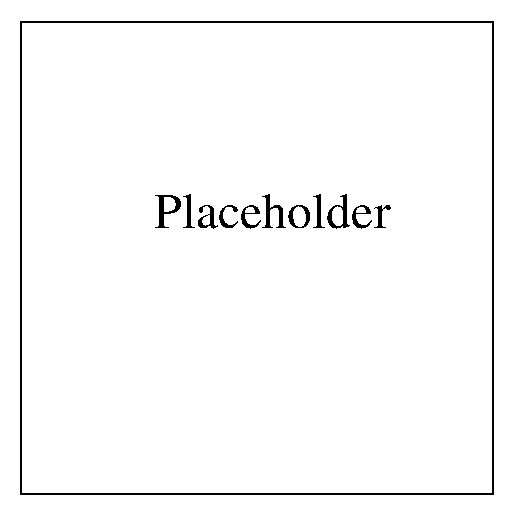
\includegraphics[width=0.40\textwidth]{figures/placeholder8x8.eps}}
%\subfloat[]{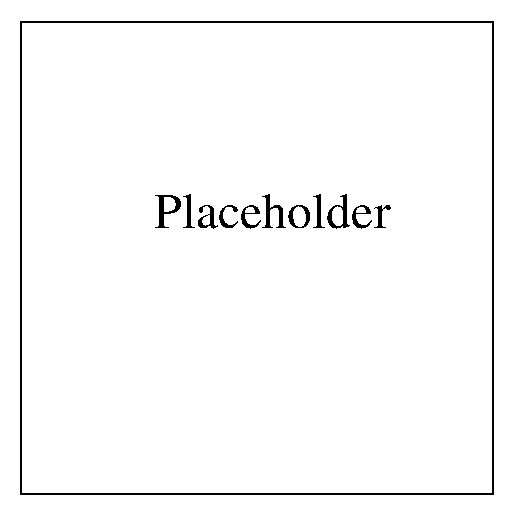
\includegraphics[width=0.40\textwidth]{figures/placeholder8x8.eps}} \\
%\subfloat[]{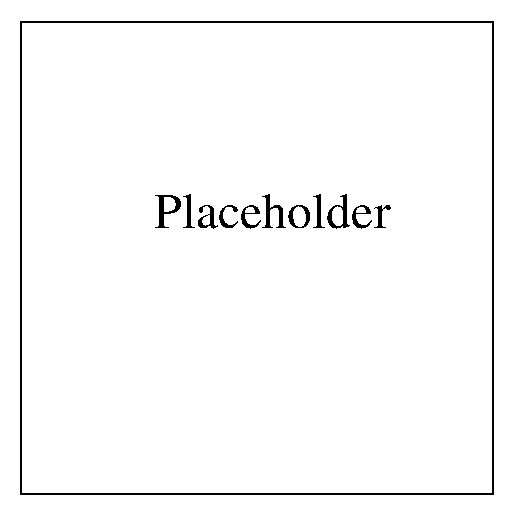
\includegraphics[width=0.40\textwidth]{figures/placeholder8x8.eps}}
%\subfloat[]{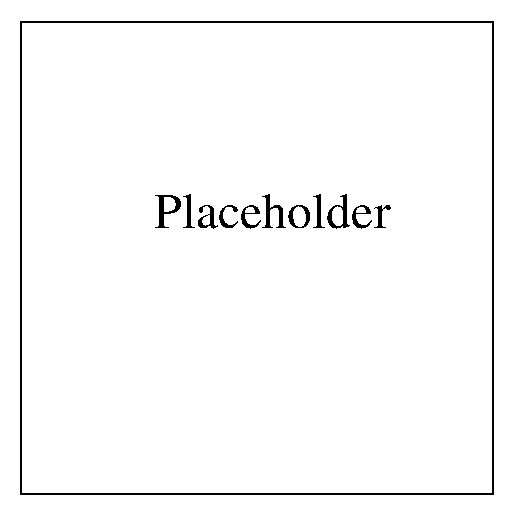
\includegraphics[width=0.40\textwidth]{figures/placeholder8x8.eps}} \\
%\caption{$\Htautau$ search: Comparison between the data and background prediction for the distribution of two of the most 
%important BDT input variables in the $\hadhad$ channel before performing the fit to data (``Pre-Fit''). The distributions are shown for
%$x_{2}^{\text{fit}}$ in (a) the ($\hadhad$, 3j) region and (b) the ($\hadhad$, $\geq$4j) region, and for
%$p_{\text{T},2}$ in (c) the ($\hadhad$, 3j)  region and (d) the ($\hadhad$, $\geq$4j) region.
%The contributions with real $\had$ candidates from $\ttbar$,  $\ttbar V$, $\ttbar H$, and single top backgrounds are combined into
%a single background source referred to as ``Top (real $\had$)", whereas the small contributions from 
%$Z\to \ell^+\ell^-$ ($\ell = e, \mu$) and diboson backgrounds are combined into ``Other''. 
%The expected $\Hc$ signal (solid red) corresponding to $\BR(t\to Hc)=1\%$ is also shown,
%added on top of the background prediction.
%The first and the last bins in the figures in (c) and (d) contain the underflow and overflow respectively.
%The bottom panel displays the ratio of data to the SM background (``Bkg'') prediction.
%The hashed area represents the total uncertainty on the background, excluding the normalisation uncertainty of the fake $\had$ background, 
%which is determined via a likelihood fit to data.} 
%\label{fig:BDT_inputs_hadhad_3}
%\end{center}
%\end{figure*}
%%%%%%%%%%%%%%%%%%%%%%%%%%%%%%%%%%%%%%%


%%%%%%%%%%%%%%%%%%%%%%%%%%%%%%%%%%%%%%%
%\begin{figure*}[t]
%\begin{center}
%\subfloat[]{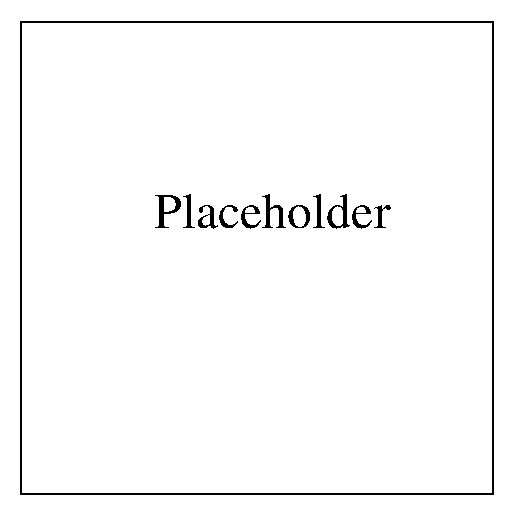
\includegraphics[width=0.40\textwidth]{figures/placeholder8x8.eps}}
%\subfloat[]{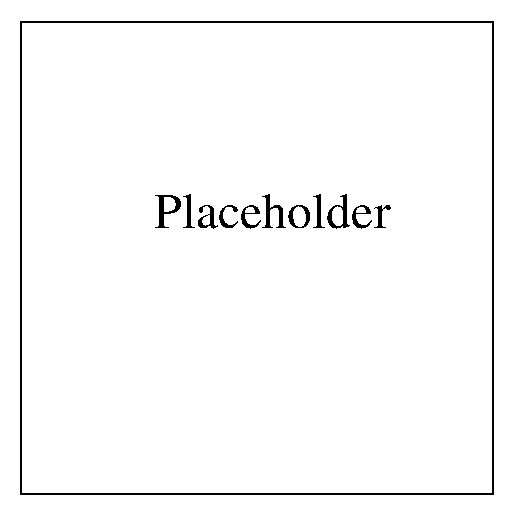
\includegraphics[width=0.40\textwidth]{figures/placeholder8x8.eps}} \\
%\subfloat[]{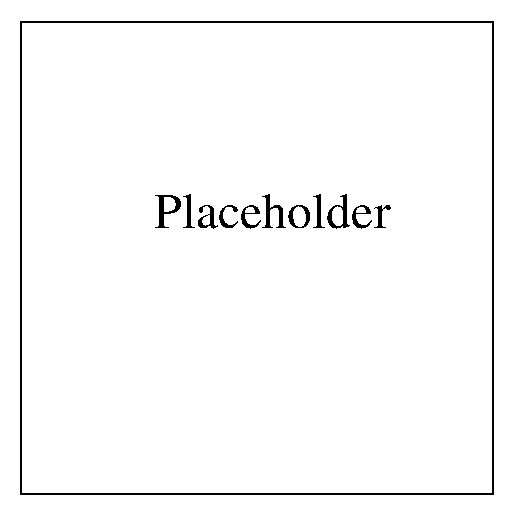
\includegraphics[width=0.40\textwidth]{figures/placeholder8x8.eps}}
%\subfloat[]{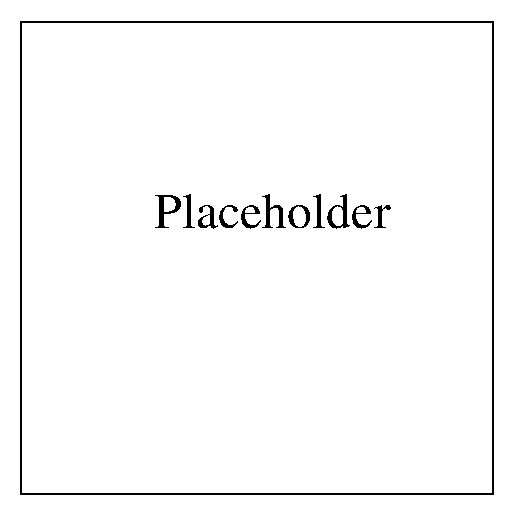
\includegraphics[width=0.40\textwidth]{figures/placeholder8x8.eps}} \\
%\caption{$\Htautau$ search: Comparison between the data and background prediction for the distribution of two of the most 
%important BDT input variables in the $\hadhad$ channel before performing the fit to data (``Pre-Fit''). The distributions are shown for
%$x_{2}^{\text{fit}}$ in (a) the ($\hadhad$, 3j) region and (b) the ($\hadhad$, $\geq$4j) region, and for
%$p_{\text{T},2}$ in (c) the ($\hadhad$, 3j)  region and (d) the ($\hadhad$, $\geq$4j) region.
%The contributions with real $\had$ candidates from $\ttbar$,  $\ttbar V$, $\ttbar H$, and single top backgrounds are combined into
%a single background source referred to as ``Top (real $\had$)", whereas the small contributions from 
%$Z\to \ell^+\ell^-$ ($\ell = e, \mu$) and diboson backgrounds are combined into ``Other''. 
%The expected $\Hc$ signal (solid red) corresponding to $\BR(t\to Hc)=1\%$ is also shown,
%added on top of the background prediction.
%The first and the last bins in the figures in (c) and (d) contain the underflow and overflow respectively.
%The bottom panel displays the ratio of data to the SM background (``Bkg'') prediction.
%The hashed area represents the total uncertainty on the background, excluding the normalisation uncertainty of the fake $\had$ background, 
%which is determined via a likelihood fit to data.} 
%\label{fig:BDT_inputs_hadhad_3}
%\end{center}
%\end{figure*}
%%%%%%%%%%%%%%%%%%%%%%%%%%%%%%%%%%%%%%%
